% This section describes the methodology of the selection
% The following sections should be here:
% - Optical Precuts
% - Optical Flash Matching
% - Cosmic Hit Removal and NuMu removal (reference marco only, really)
% - Preselection with 1+tracks, 1+showers OR 2+ showers
% - Pion and Muon Rejection in tracks (AKA, proton selection)
% - Background Rejection Cuts

\section{Analysis Methodology}
\label{sec:methodology}

% This section will describe the methodology used in this analysis, and the details of some of the technical aspects of the methodology (optical flash matching, dE/dx calculation, proton PID, etc).  Some of the cuts of the analysis that are well developed and static are described in this section, for example the optical precuts.  Other cuts, such as the background rejection cuts applied after the preselections, are described in Section~\ref{sec:electron_like} though the techniques used to calculated these variables are described here.

In the TPC, ionisation electrons passing through the MicroBooNE cryostat are drifted to the anode, inducing electric signals on the wires of the three TPC planes. The waveforms observed for each wire are examined and a hit-finding algorithm searches for local maxima and minima. A Gaussian distribution is fitted to each peak and hit objects are created. The hits are used by the reconstruction algorithms provided by the Pandora framework \cite{pandora} to form TPC reconstructed objects. 

The Pandora reconstruction produces as a first stage a list of two-dimensional clusters, which represent continuous, unambiguous lines of hits. Thus, cluster-merging algorithms identify associations between multiple clusters. The three-dimensional track and shower reconstruction then collects the two-dimensional clusters from the three readout planes that represent individual, track-like or shower-like objects \cite{pandora2}. Our analysis relies on these high-level reconstructed objects to select our CC0$\pi$-Np candidates.

MicroBooNE is also equipped with an optical system made of 32 photomultipliers tubes placed behind the anode plane, with few-ns timing resolution. The optical system detects the argon scintillation light produced by the neutrino interaction and it provides the TPC start time of the event.
Figure \ref{fig:evd} shows a simulated event display of one wire plane with an electron and two protons in the final state, with the corresponding reconstructed shower and reconstructed tracks. In this case, the algorithm was able to correctly reconstruct the electromagnetic shower and both proton tracks.

\begin{figure}[htbp]
	\begin{center}
    	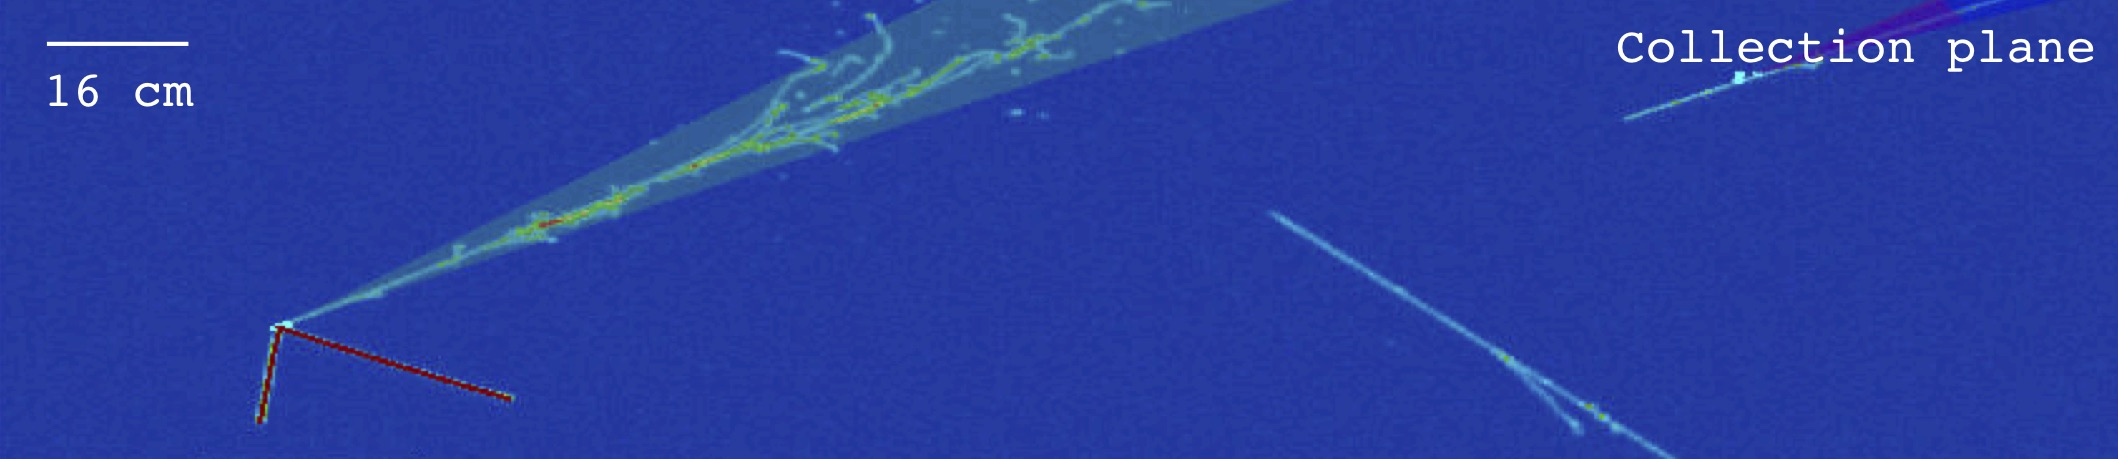
\includegraphics[width=0.8\linewidth]{figures/evd.jpg}
    	\caption{Monte Carlo event display of the collection plane with an electron and two protons in the final state. The reconstructed shower-like object is represented by the green cone. The reconstructed track-like objects are represented by the red lines.} \label{fig:evd}
	\end{center}
\end{figure}

% Our $\nu_{e}$ CC0$\pi$-Np selection algorithm first looks for (1) a flash in the optical system compatible with one of the neutrino interaction candidates provided by the Pandora framework, plus (2) a neutrino interaction candidate with one or more track-like objects and one or more shower-like objects, or two or more shower-like objects. 
% Then, the $\nu_{\mu}$ and cosmic-ray candidates selected by an external module \cite{ubxsec} are removed from the sample. The signal events  Finally, the energy spectrum of the $\nu_{e}$ CC0$\pi$-Np candidates is measured with the procedure described in Section \ref{sec:energyreco}.

\subsection{Overview}

In order to reconstruct the spectrum of the $\nu_{e}$ CC0$\pi$-Np events collected by the MicroBooNE experiment, this analysis has been divided into several, broadly linear stages:
\begin{enumerate}
\item Optical pre-cuts and flash-matching: a minimum amount of photoelectrons in the optical system is required. At least one of the neutrino candidates provided by the Pandora framework must be then compatible with the flash in the optical system.
\item Electron neutrino topological pre-selection: one of the neutrino candidates must be compatible with the topology of a $\nu_{e}$ CC0$\pi$-Np interaction, that is at least one track and at least one shower or at least two showers sharing a common vertex.
\item CC $\nu_{\mu}$ neutrino and cosmic-ray candidates removal: events tagged as CC $\nu_{\mu}$ neutrino candidates or non-neutrino induced are vetoed by an external module.
\item Background rejection through calorimetric and geometric cuts: $\nu_{e}$ CC0$\pi$-Np events are further isolated applying several boxed cuts on kinematic, geometric, and calorimetric variables. The electromagnetic showers initiated by an electron in the final state are isolated with a cut on the $dE/dx$ value. The proton tracks are selected with a Boosted Decision Tree trained on the track $dQ/dx$ and its length.
\item Energy spectrum reconstruction: the energy of the electron showers is measured with a hit-based procedure, while the energy deposited by the proton tracks is calculated from the length of the reconstructed track. 
\end{enumerate}

\subsection{Cosmic Hit Removal}
Being located almost on surface, the MicroBooNE detector is constantly hit by atmospheric cosmic rays, at a rate of $\approx5$~kHz \cite{cosmic}. These cosmic rays will interact in the TPC, producing a combination of track-like and shower-like objects. 
In order to suppress this cosmogenic background, the Pandora framework runs in two different modes with different settings \cite{pandora}: (1) \texttt{pandoraCosmic}, optimized for cosmic rays reconstruction, and (2) \texttt{pandoraNu}, optimized for neutrino interactions reconstruction.
The reconstructed hits are first fed to the framework in the \texttt{pandoraCosmic} mode. Then, a series of cosmic-ray tagging algorithms are applied to the objects reconstructed by Pandora in this mode \cite{ubxsec}. The reconstructed hits that are deemed to be of cosmic origin by the tagging algorithms are removed from the hit collection. The remaining hits are then fed again to the framework in the \texttt{pandoraNu} mode, which reconstructs the neutrino interaction candidates.

\subsection{Optical Pre-Cuts}\label{sec:optical_pre_cuts}

The first requirement ensures the presence of light in the detector in a position compatible with the center of the collected charge of the neutrino interaction candidate and with a timing compatible with the beam-gate window.

It is also possible and likely that an event will have multiple neutrino candidates. The goal of the optical selection is reducing the number of candidates to maximal one candidate in each event. This process consists of three major parts:
\begin{enumerate}
\item Rectangular cuts are applied to optical properties of the reconstructed flash object.
\item Rectangular cuts on the compatibility of the reconstructed flash with the Pandora neutrino candidate.
\item The Pandora neutrino candidate which is most compatible with the flash is picked using a likelihood method.
\end{enumerate}

To demonstrate the effect of the used cuts, they will be applied on two different samples, both of which were produced with Monte Carlo Challenge 8.3:
\begin{itemize}
\item The signal sample: BNB $\nu_e$ intrinsic with cosmic rays
\begin{itemize}
\item The truth vertex should be in the fiducial volume.
\item There should be an electron with a kinetic energy of at least \SI{20}{\MeV}.
\item There should be at least one proton wit a kinetic energy of \SI{40}{\MeV} or higher.
\end{itemize}
\item The background sample: CORSIKA in-time cosmic rays
\end{itemize}

\begin{figure}[!htbp]
\centering
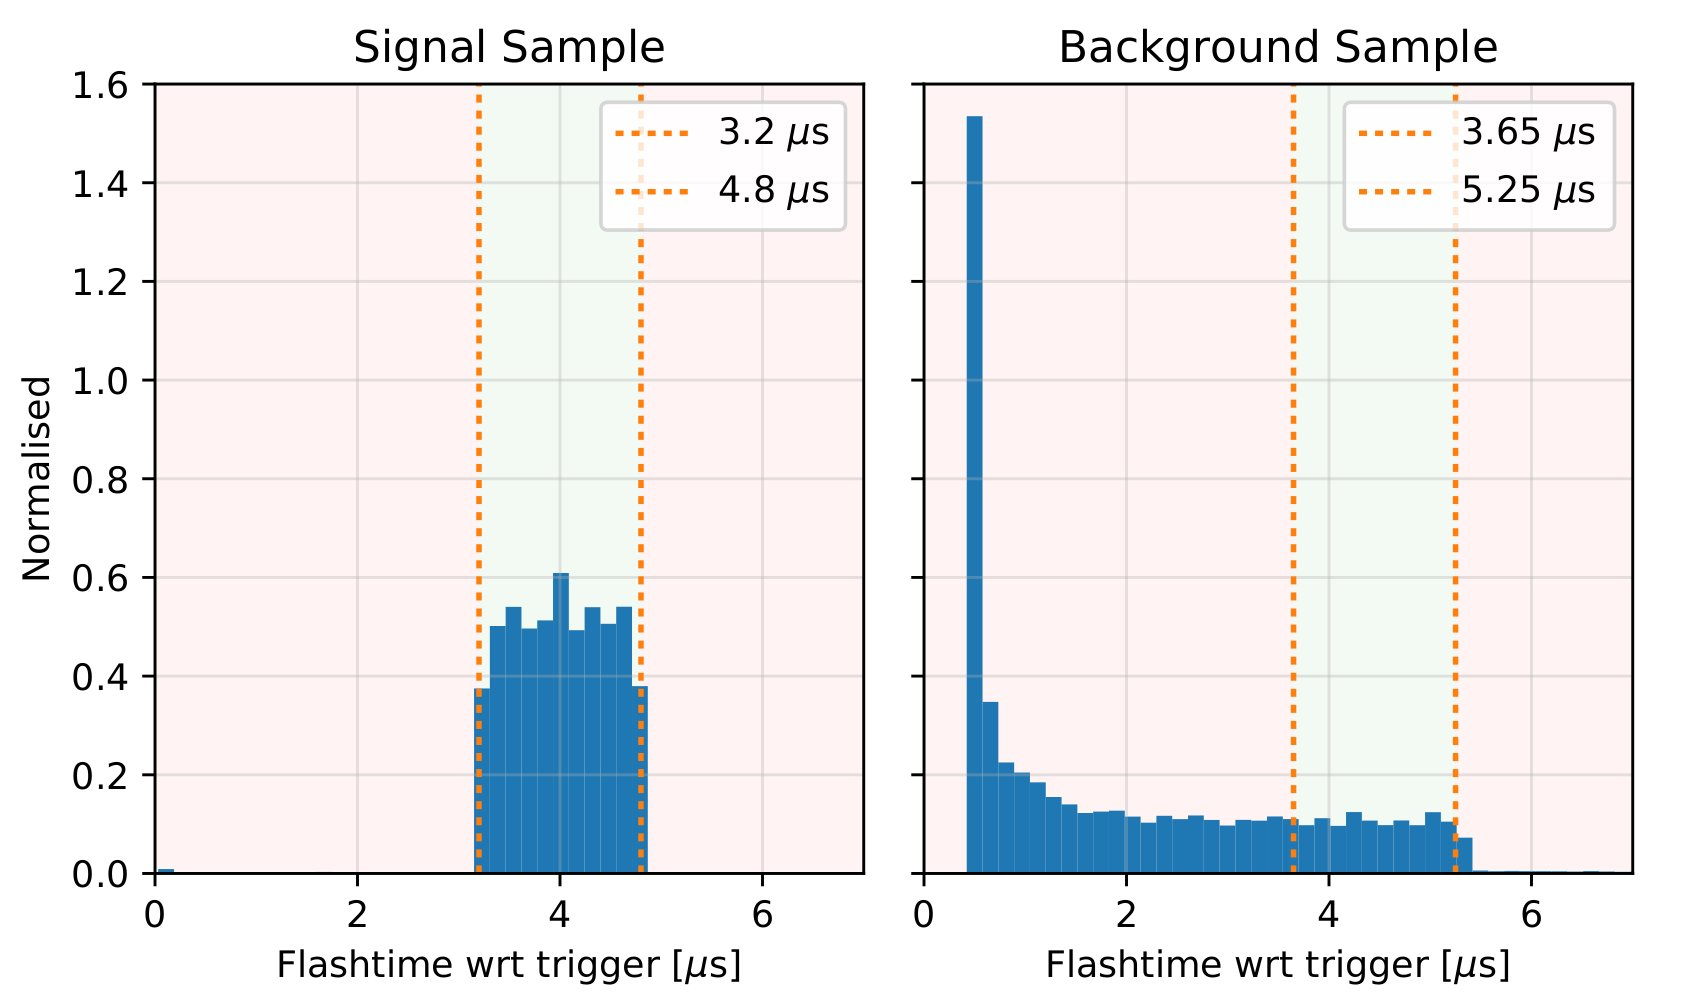
\includegraphics[width=0.75\textwidth]{beam}
\caption{Requirement a reconstructed flash object within the beam spill time window.} 
\label{fig:beam}
\end{figure}

The first requirement is that there is a reconstructed flash within the beam spill window of \SI{1.6}{\micro\s}. This cut is shown in Figure~\ref{fig:beam}. 99.6\% in the signal sample passes, 18.5\% in the background sample passes.

\begin{figure}[htbp]
\centering
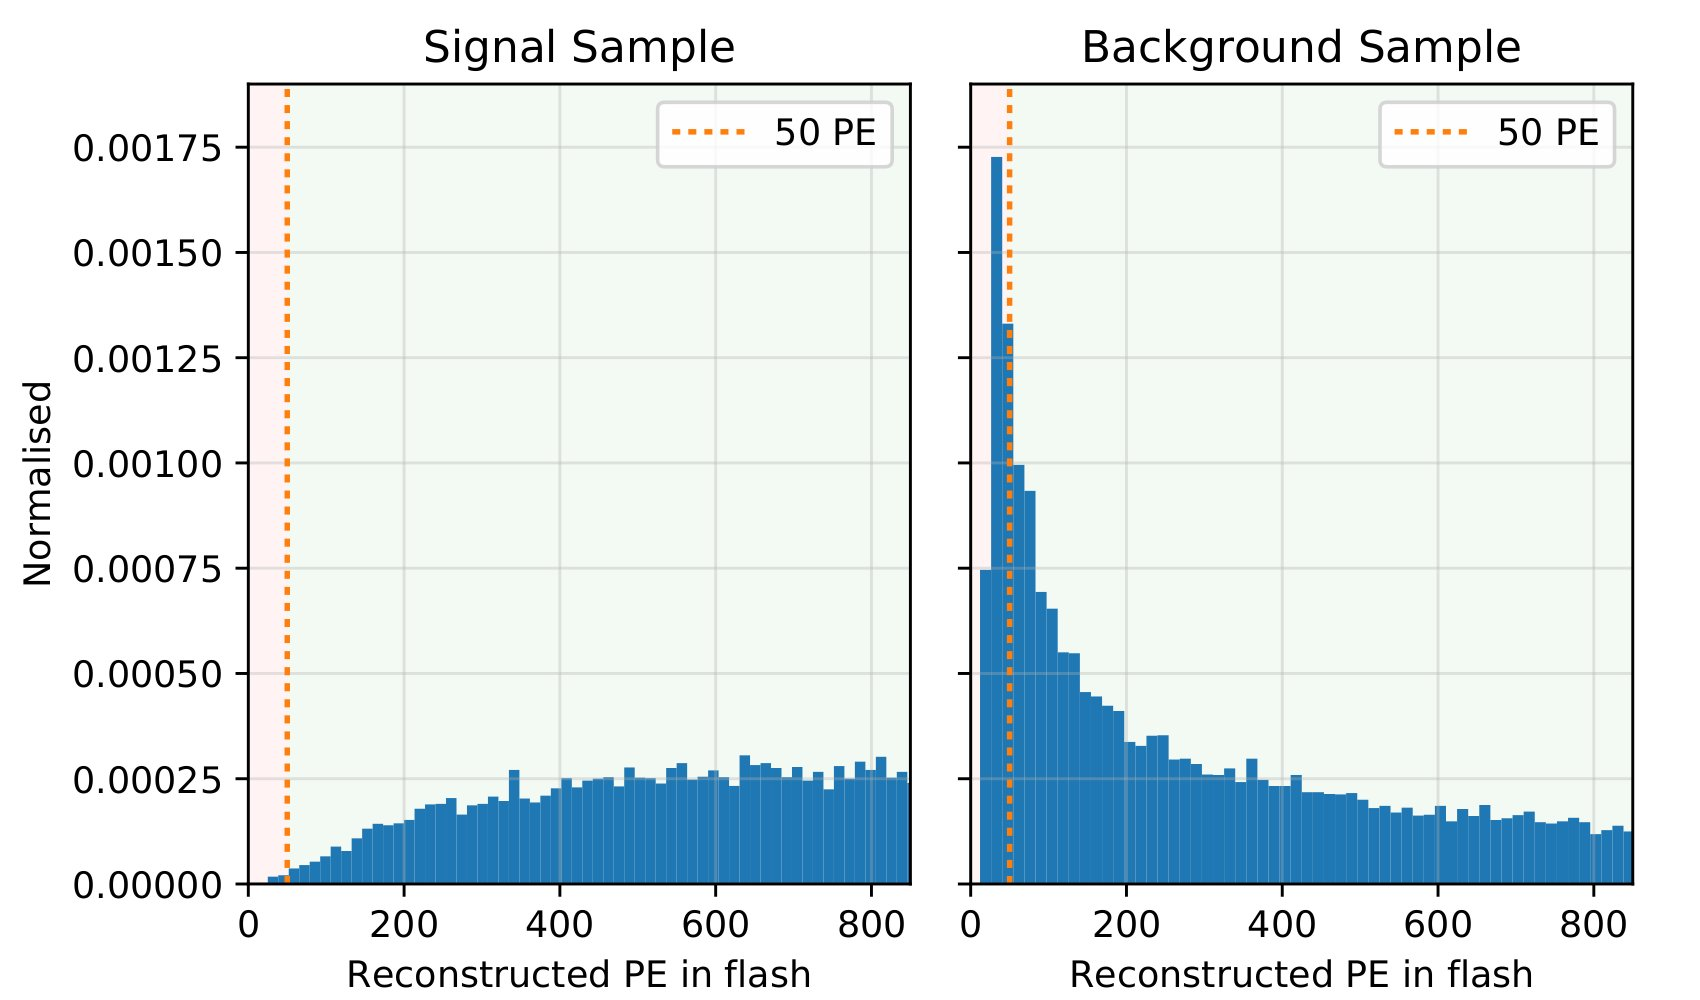
\includegraphics[width=0.75\textwidth]{PE}
\caption{Intensity of the reconstructed flash in photo-electrons. A cut is placed at 50 PE.} 
\label{fig:PE}
\end{figure}

After that, the reconstructed flash is required to consist of at least 50 photo-electrons (PE). This is a very conservative cut and keeps 99.95\% of the signal while 95.2\% of the background passes too. The PE distributions are given in Figure~\ref{fig:PE}.


\subsection{Optical Flash Matching}

At this point it is guaranteed that the event has a properly reconstructed flash. A flash object has a time and a PE count for each of the 32 PMT's. From that, a position $Z\pm \sigma_Z$ and $Y\pm \sigma_Y$ are calculated. These can be compared with the. centre of deposited charge of the Pandora candidate. This comparison has the implicit assumption that the light will be emitted in the same relative fraction as the charge is deposited by the final state particles. This is not completely correct since the amount of scintillation light produced per deposited \SI{1}{\MeV} is particle dependent. Nevertheless, compared to the coarse resolution of the PMT grid, this approximation is justified. 

\begin{figure}[htbp]
\centering
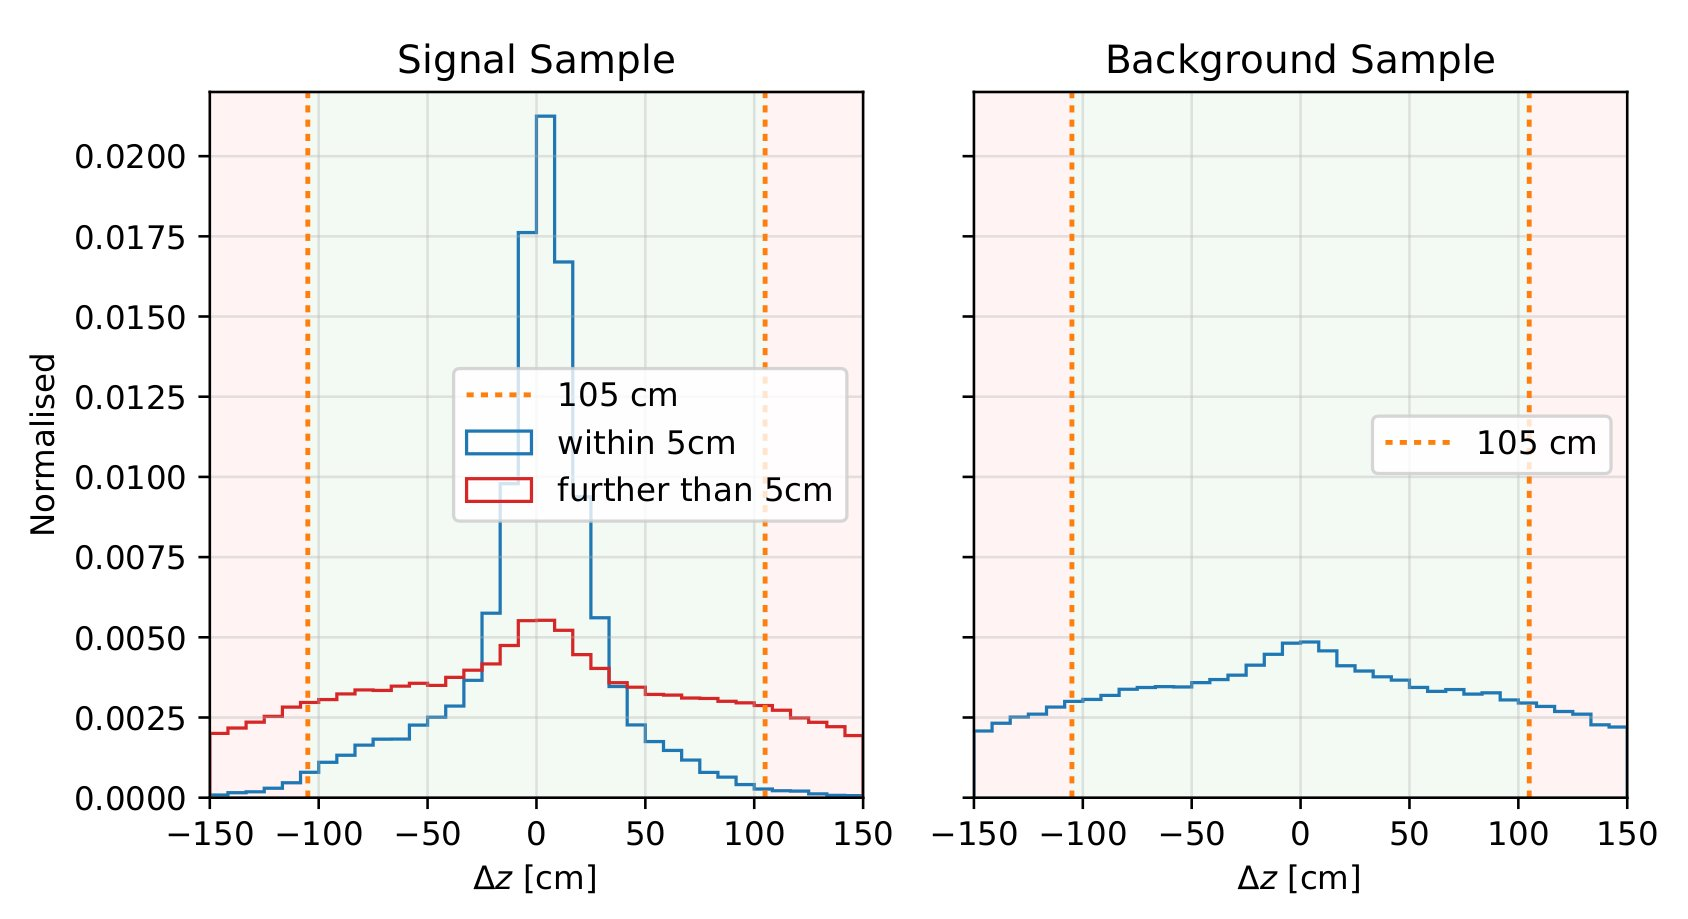
\includegraphics[width=0.8\textwidth]{zcut}
\caption{The distance between the flash and centre of deposited charge of the Pandora neutrino candidate. It is required that this is less than \SI{105}{\cm}.} 
\label{fig:zcut}
\end{figure}

In Figure~\ref{fig:zcut}, The effect of this cut is demonstrated. The signal sample is split up in two categories using truth information. Pandora neutrino candidates with their reconstructed vertex within \SI{5}{\cm} from the true vertex, and Pandora neutrino candidates with their reconstructed vertex further away. Those candidates with a mis-reconstructed vertex are often related to cosmic interaction, either mixed with neutrino activity or pure background. We therefore expect this group in the signal sample to follow the distribution of the background sample, which is confirmed in the figure. A cut is placed on a difference of \SI{105}{\cm} difference between the reconstructed flash position and the position of the deposited charge. This cut keeps at least one neutrino candidate in 98.1\% of the signal while it removes all neutrino candidates in 20\% of the background event. 
Similar cuts are obtained taking into account the width of the flash and the $y$-position. 

\begin{figure}[!htbp]
\centering
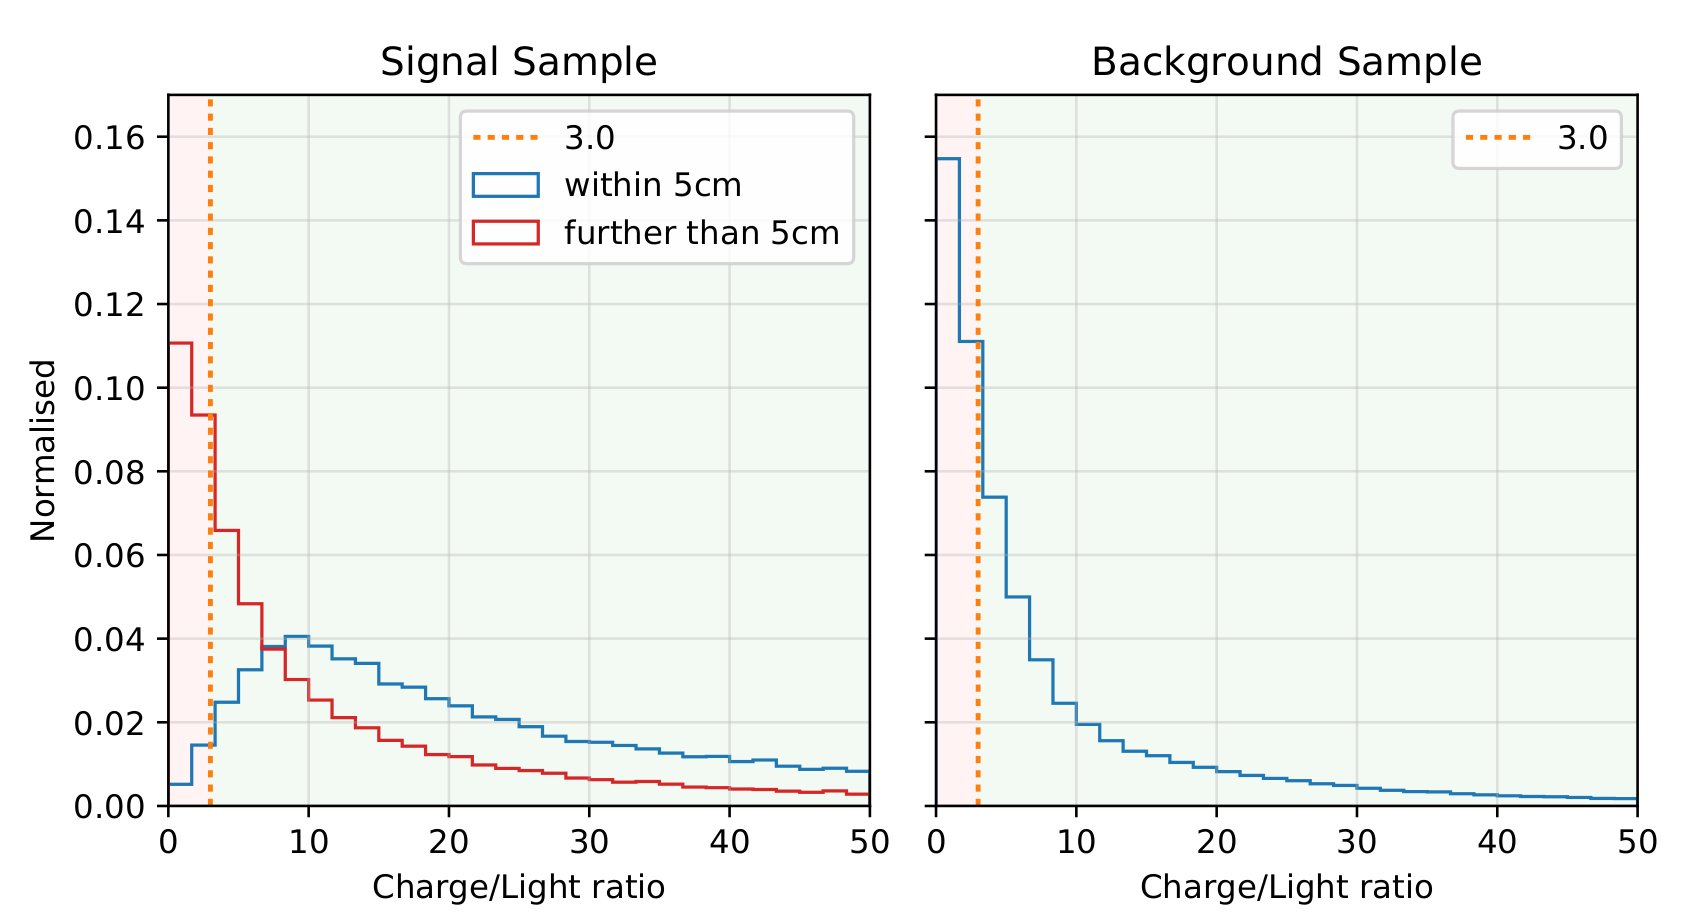
\includegraphics[width=0.8\textwidth]{charge}
\caption{For neutrino interactions, the a higher amount of deposited charge will come together with a more intense reconstructed flash. A cut on the ratio of higher than 3.0 is imposed on the neutrino candidates.} 
\label{fig:charge}
\end{figure}

The last rectangular cut exploits the fact that a lot of the neutrino candidates reconstructed by Pandora originate from remainders of cosmic activity that was not completely removed in the cosmic removal stage of the reconstruction. Those neutrino candidates often consist of a small amount of fragmented charge, incompatible with the brightness of the flash. In Figure~\ref{fig:charge}, the ratio of deposited charge associated to a neutrino candidate and the  amount of photo-electrons in the reconstructed flash is shown. The signal sample is again split up in two categories as before. Placing a very conservative cut at 3.0 reduces the signal events with a properly reconstructed flash with 1.7\% while removing all neutrino candidates in 15.4\% of the events. 

\begin{figure}[!htbp]
\centering
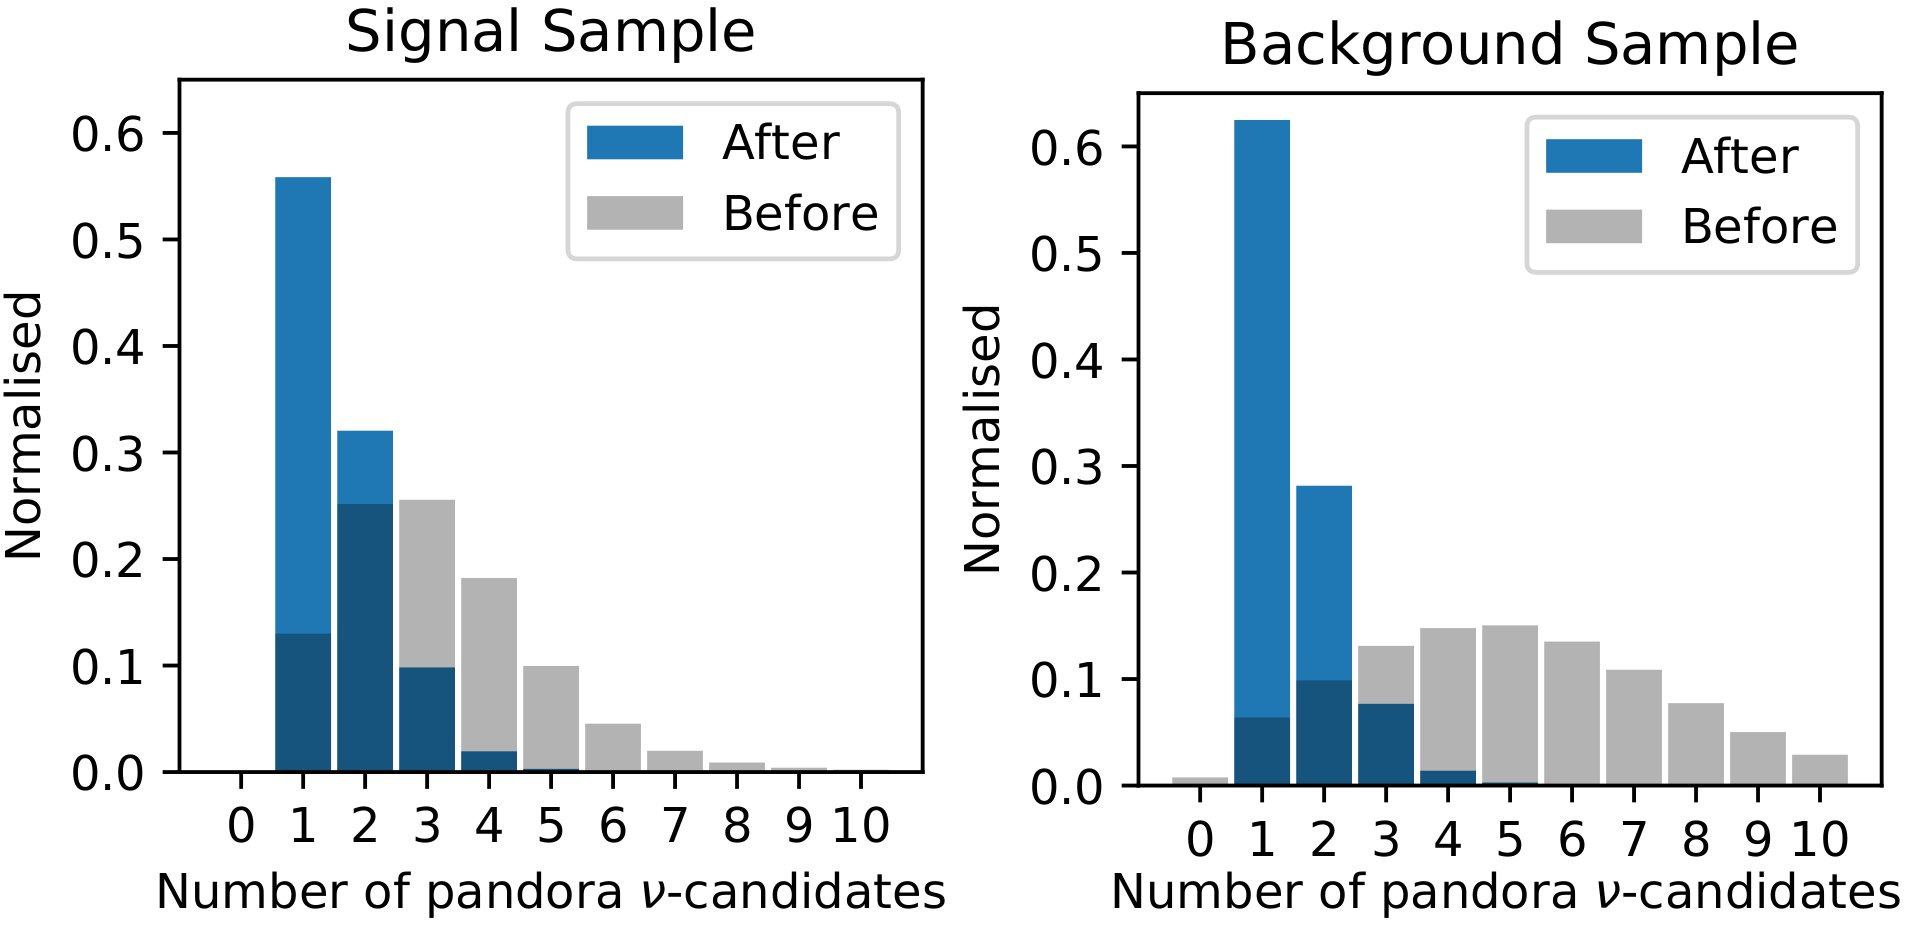
\includegraphics[width=0.8\textwidth]{boxed}
\caption{Effect of the rectangular optical cuts on the amount of Pandora neutrino candidates .} 
\label{fig:boxed}
\end{figure}

After applying the two sets of described rectangular cuts. It is informative to not only discuss the passing rates, but also the number of neutrino candidates remaining in the passed events. This is shown in Figure~\ref{fig:boxed}. In Grey, the number of neutrino candidates before any cuts is shown. In blue, the number of candidates that passed the rectangular cuts is shown. In about half of the remaining cases, there are multiple neutrino candidates remaining, this will be reduced to exactly one per passing event using flash-matching. 

\begin{figure}[!htbp]
\centering
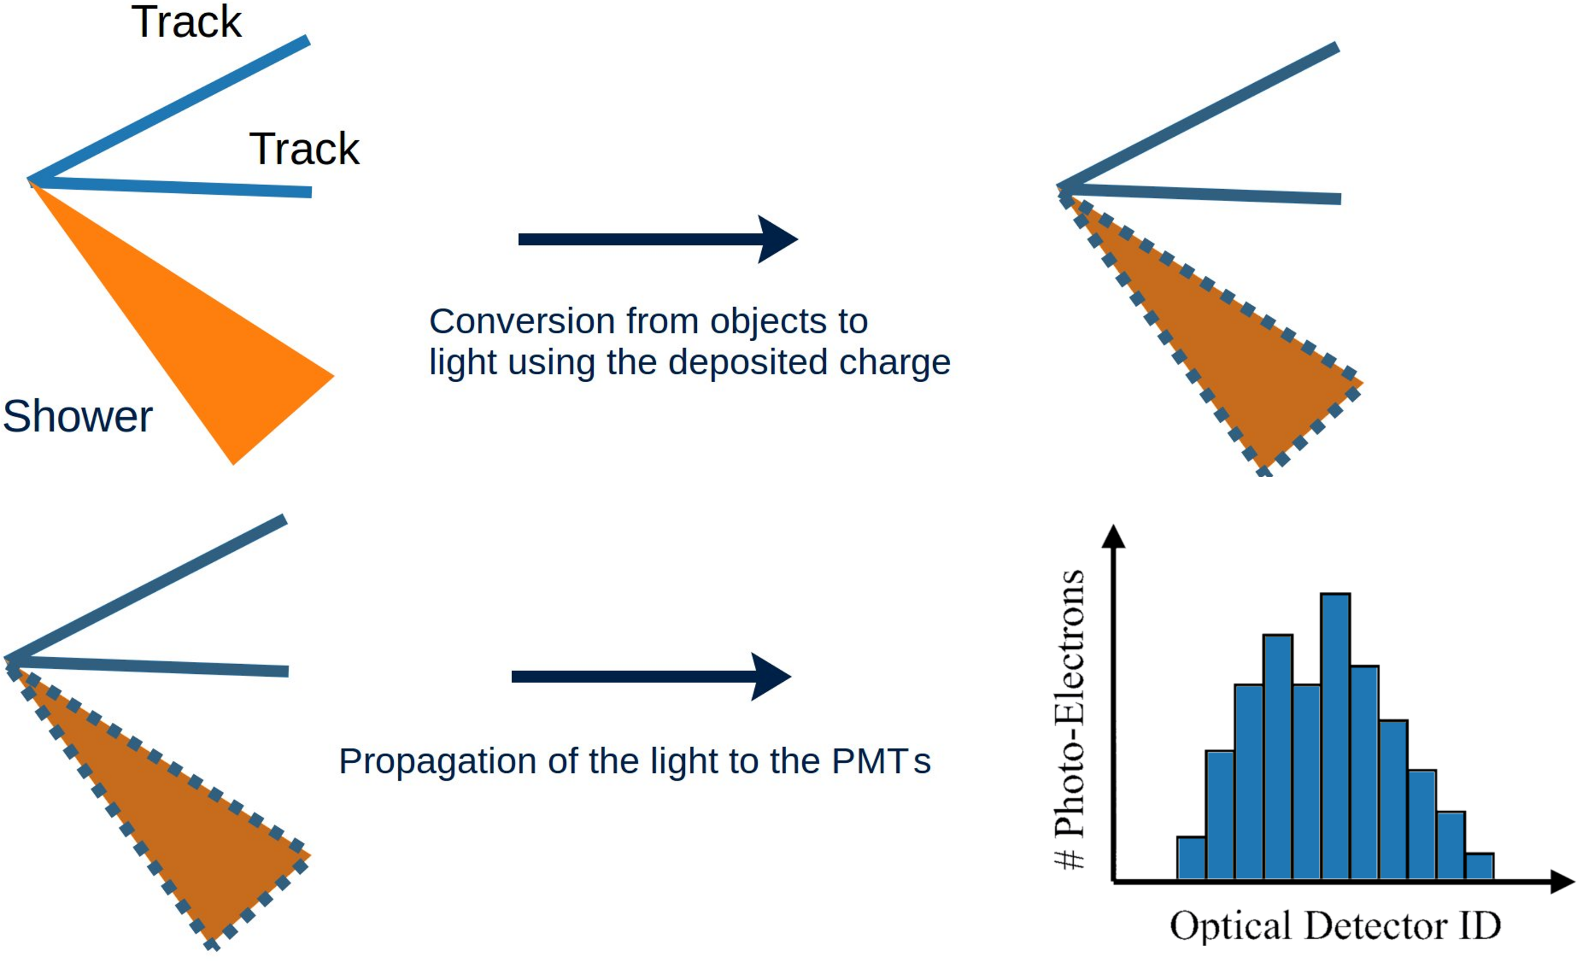
\includegraphics[width=0.7\textwidth]{flashdrawing} 
\caption{Schematic of the construction of a flash hypothesis for a neutrino candidate.} 
\label{fig:flashdrawing}
\end{figure}

The principle of flash-matching is described in Figure~\ref{fig:flashdrawing}:
\begin{itemize}
\item A flash hypothesis can be constructed for each candidate vertex using only data recorded by the time projection chamber.
\item For every neutrino candidate, a spatial distribution of deposited charge can be constructed.
\item The spatial distribution of the deposited charge is translated into an estimation of the emitted scintillation light. These scintillation photons are then propagated towards the PMTs to construct a flash hypothesis using only time projection chamber information.
\item The flash-matching algorithm compares the reconstructed flash object as seen by the PMT's with the hypothetical flash for all possible neutrino candidates and picks the best matching candidate. For this, a binned likelihood of the PMT spectrum is optimised.
\end{itemize}
An example of this procedure for a Monte Carlo generated $\nu_e$ event with 4 neutrino candidates is given in Figure~\ref{fig:flashmatch}.
\begin{figure}[!htbp]
\centering
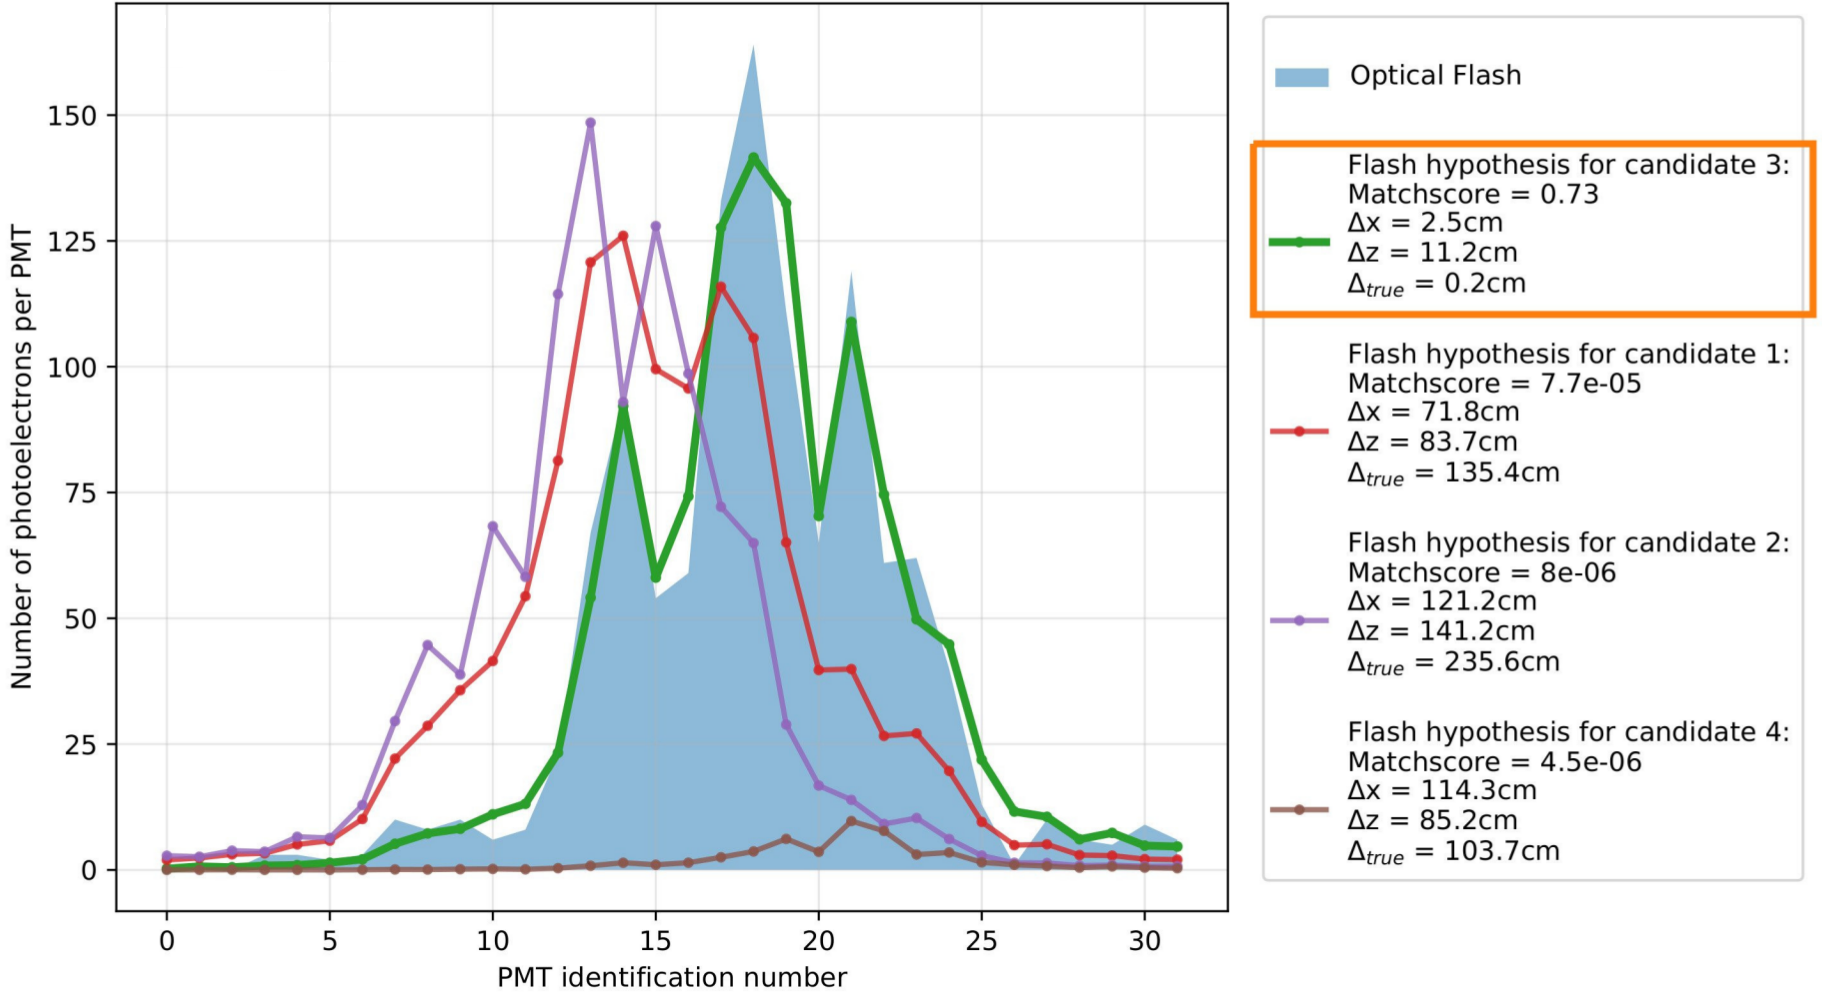
\includegraphics[width=0.85\textwidth]{flashmatch} 
\caption{An example of flash-matching. Event with 4 neutrino candidates, for all of the candidates the flash hypothesis is constructed and matched to the reconstructed flash (shaded blue). For all candidates a minimum binned likelihood is calculated, varying the $x$ position of the interaction. The match score is the inverse of the likelihood. For all neutrino candidates, the reconstructed vertex is compared with the true distance and given by $\Delta_{true}$ } 
\label{fig:flashmatch}
\end{figure}

\subsection{Electron Neutrino Topological Pre-Selection}\label{sec:topological_pre_selection}
A perfect reconstruction of a $\nu_{e}$ CC0$\pi$-Np event in a LArTPC will produce as many reconstructed tracks as the number of protons in the final state and a single reconstructed shower (the electron), sharing a common vertex. However, the presence of missing or unresponsive wires can cause the splitting of an ionization track or an electromagnetic showers into two distinct reconstructed object. Also, the type of object (track or shower) is assigned by a Support Vector Machine (SVM) implemented in the Pandora framework and its performances depend on the quality of the event (e.g. the number of hits). A track-like object (e.g. a proton or a muon), then, can be mis-reconstructed as a shower-like object, especially when the number of reconstructed hits is low \cite{pandora2}. In order to maximize our efficiency, then, we will require (1) \emph{at least} one track and \emph{at least} one shower sharing a common vertex, or (2) \emph{at least} two showers sharing a common vertex. Figure \ref{fig:dia} shows the two diagrams of the accepted topologies for a $\nu_{e}$ CC0$\pi$-Np candidate event.

\begin{figure}[htbp]
\centering
  \begin{subfigure}{0.4\textwidth}
    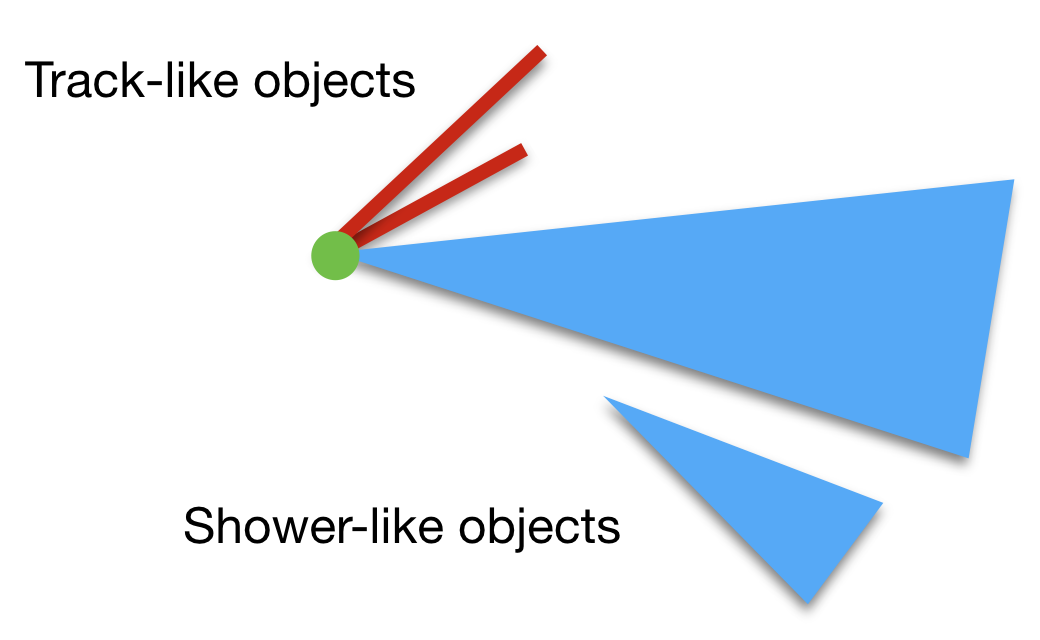
\includegraphics[width=\linewidth]{figures/trsh.png}
    \caption{1+ tracks and 1+ showers} 
  \end{subfigure}
    \begin{subfigure}{0.4\textwidth}
    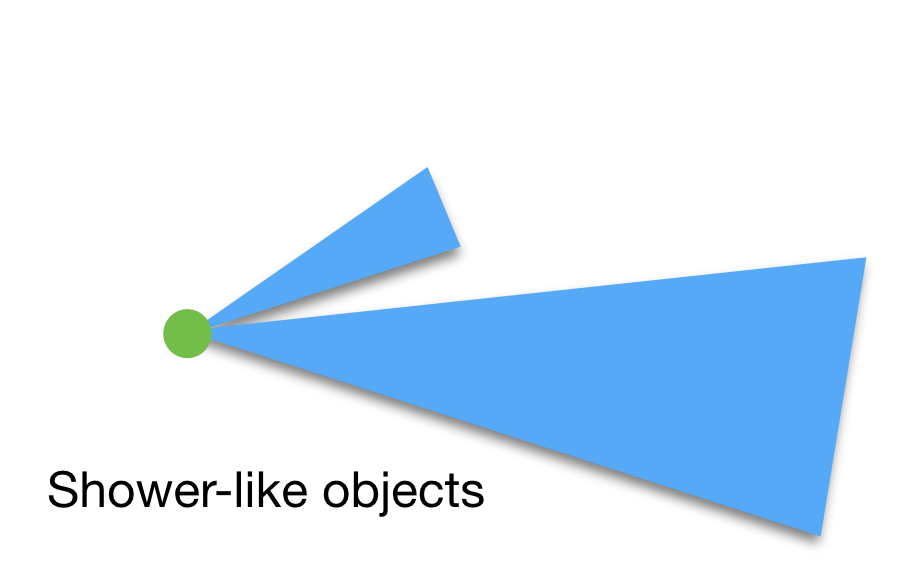
\includegraphics[width=\linewidth]{figures/sh.png}
    \caption{2+ showers} 
  \end{subfigure}
  \caption{The $\nu_{e}$ topological pre-selection requires a neutrino candidate with one or more tracks and one or more shower sharing (left) or two or more showers (right) sharing  a common vertex.}\label{fig:dia}
\end{figure}

Figure \ref{fig:2showers} shows a Monte Carlo event display with an electromagnetic shower correctly reconstructed as a shower-like object and a proton track mis-reconstructed as a shower-like object. Requiring at least two showers allows to recover this kind of event.

\begin{figure}[htbp]
	\begin{center}
    	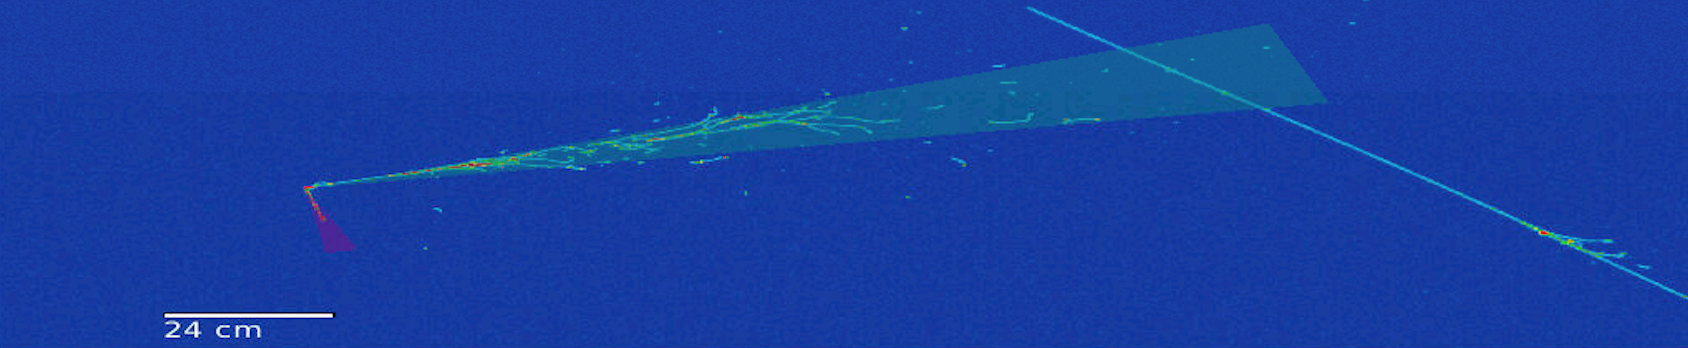
\includegraphics[width=0.8\linewidth]{figures/2showers.png}
    	\caption{Monte Carlo event display of the collection plane with one electron and one proton in the final state. The proton track has been mis-reconstructed as a shower-like object.} \label{fig:2showers}
	\end{center}
\end{figure}

In these cases, in order to choose the proton track candidate among the two or more shower-like objects, we run a bi-dimensional Principal Component Analysis in the collection plane (one dimension is given by the drift time and the other by the wire coordinate). The object with the largest first eigenvalue is chosen as the proton track candidate and it is then considered as a track-like object.

\subsubsection{Selection efficiency and purity}\label{sec:eff}
A first estimate of the number of events that can be selected by our algorithm is obtained by measuring the selection efficiency and purity using a dedicated $\nu_{e}$ CC$0\pi$-Np Monte Carlo sample. Neutrino events have been generated using the GENIE Neutrino Monte Carlo generator \cite{genie} and cosmic rays have been generated using the CORSIKA Monte Carlo generator \cite{corsika}. 

In this sample, every event has one $\nu_{e}$ interaction with one electron, at least one proton and no other visible particles in the final state (it can have neutrons). 

In order to avoid border effects, such as electric field non-uniformities, the true neutrino interaction vertex must lie within a fiducial volume. Our fiducial volume cut is $\pm10$~cm on the $x$ axis, $\pm20$~cm on the $y$ axis, and $^{+10}_{-50}$~cm on the $z$ axis. 
Since electromagnetic showers develop mainly in the forward direction with respect to the beam, the asymmetric cut on the $z$ axis (which corresponds to the beam direction) helps reject non-fully contained events.

A study on the reconstruction efficiency of proton tracks and electron showers in $\nu_{e}$ CC$0\pi$-Np events shows that the efficiency is zero for proton with a kinetic energy below 40~MeV and for electrons with a kinetic energy below 20~MeV. As such, in our sample each event must have at least one proton above 40~MeV and one electron above 20~MeV. Figure \ref{fig:kin_eff} shows the reconstruction efficiencies for protons and electrons as a function of the kinetic energy.

\begin{figure}[htbp]
  \begin{subfigure}{0.48\textwidth}
    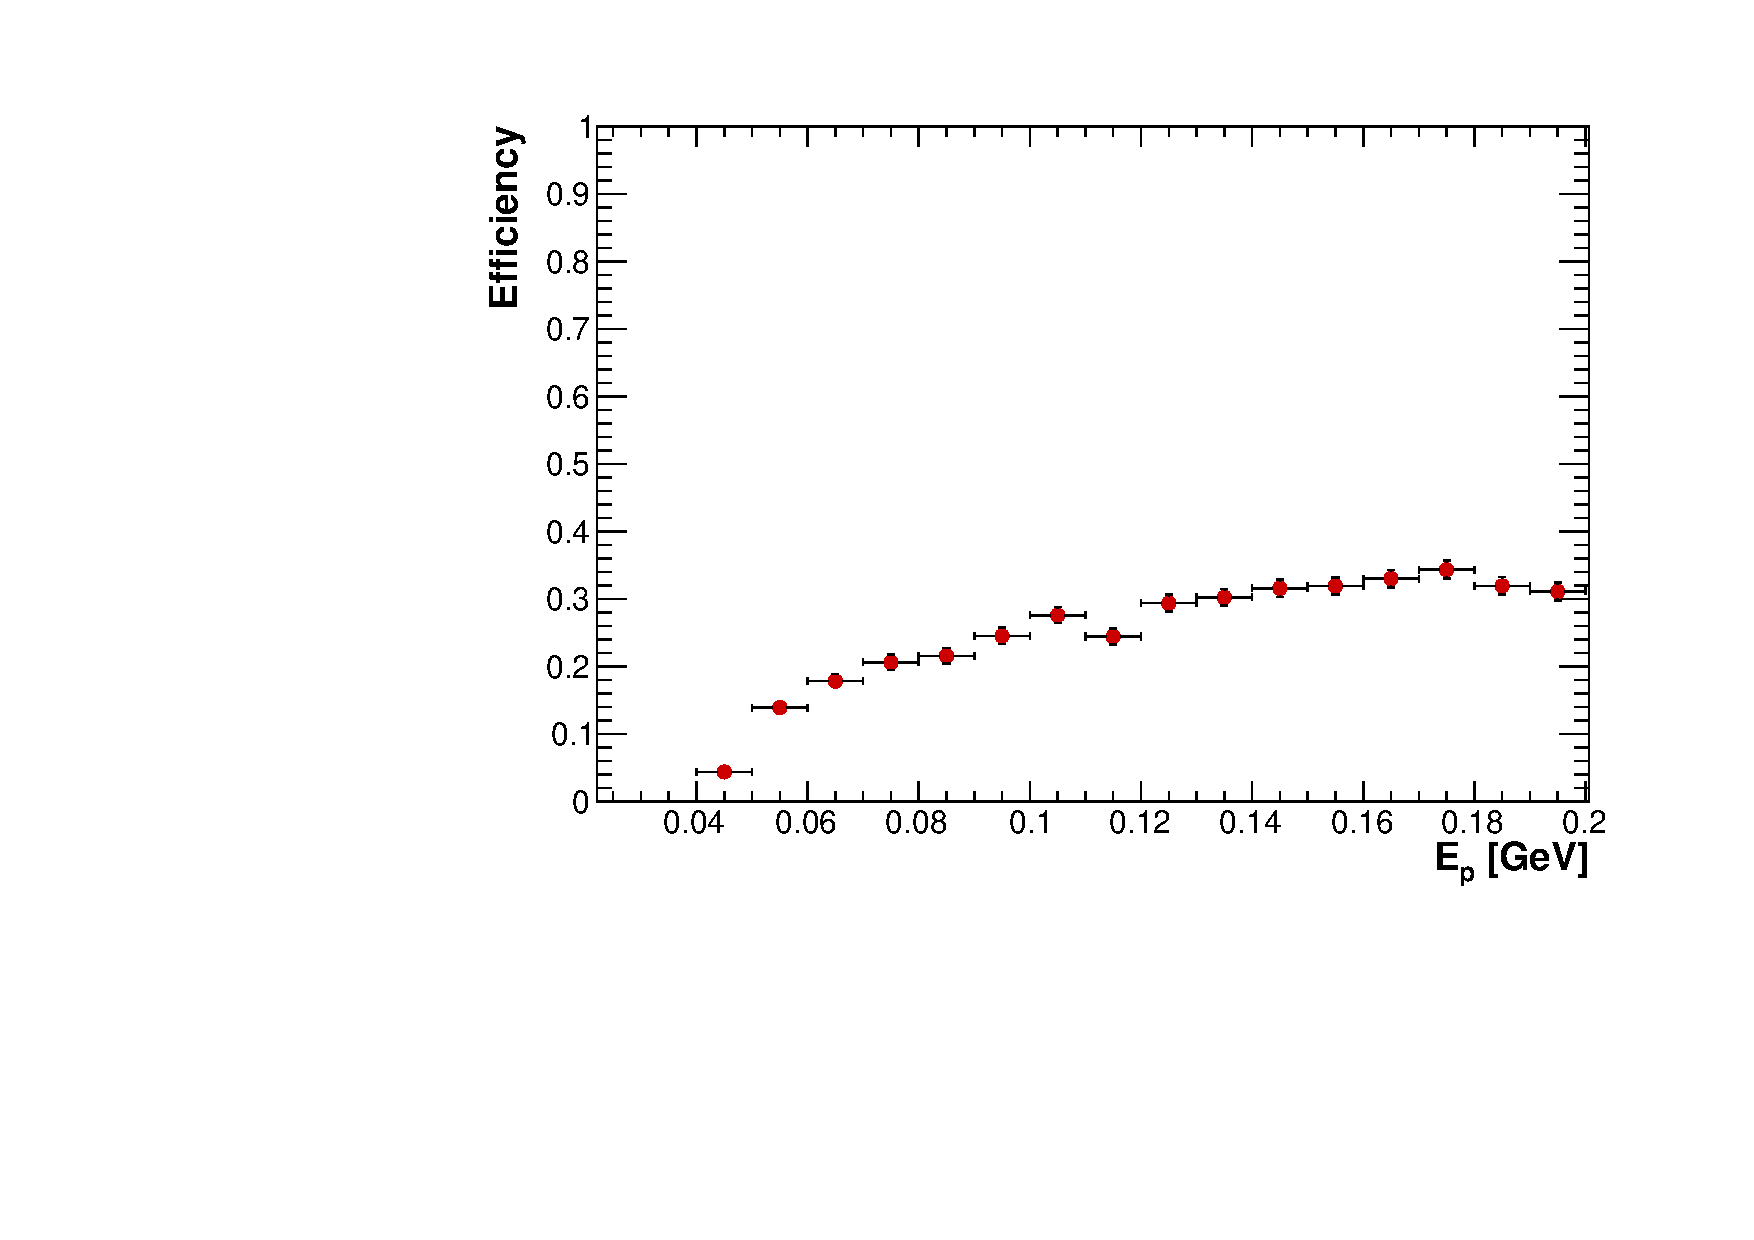
\includegraphics[width=\linewidth]{figures/proton_eff.pdf}
    \caption{Proton reconstruction efficiency} 
  \end{subfigure}
    \begin{subfigure}{0.48\textwidth}
    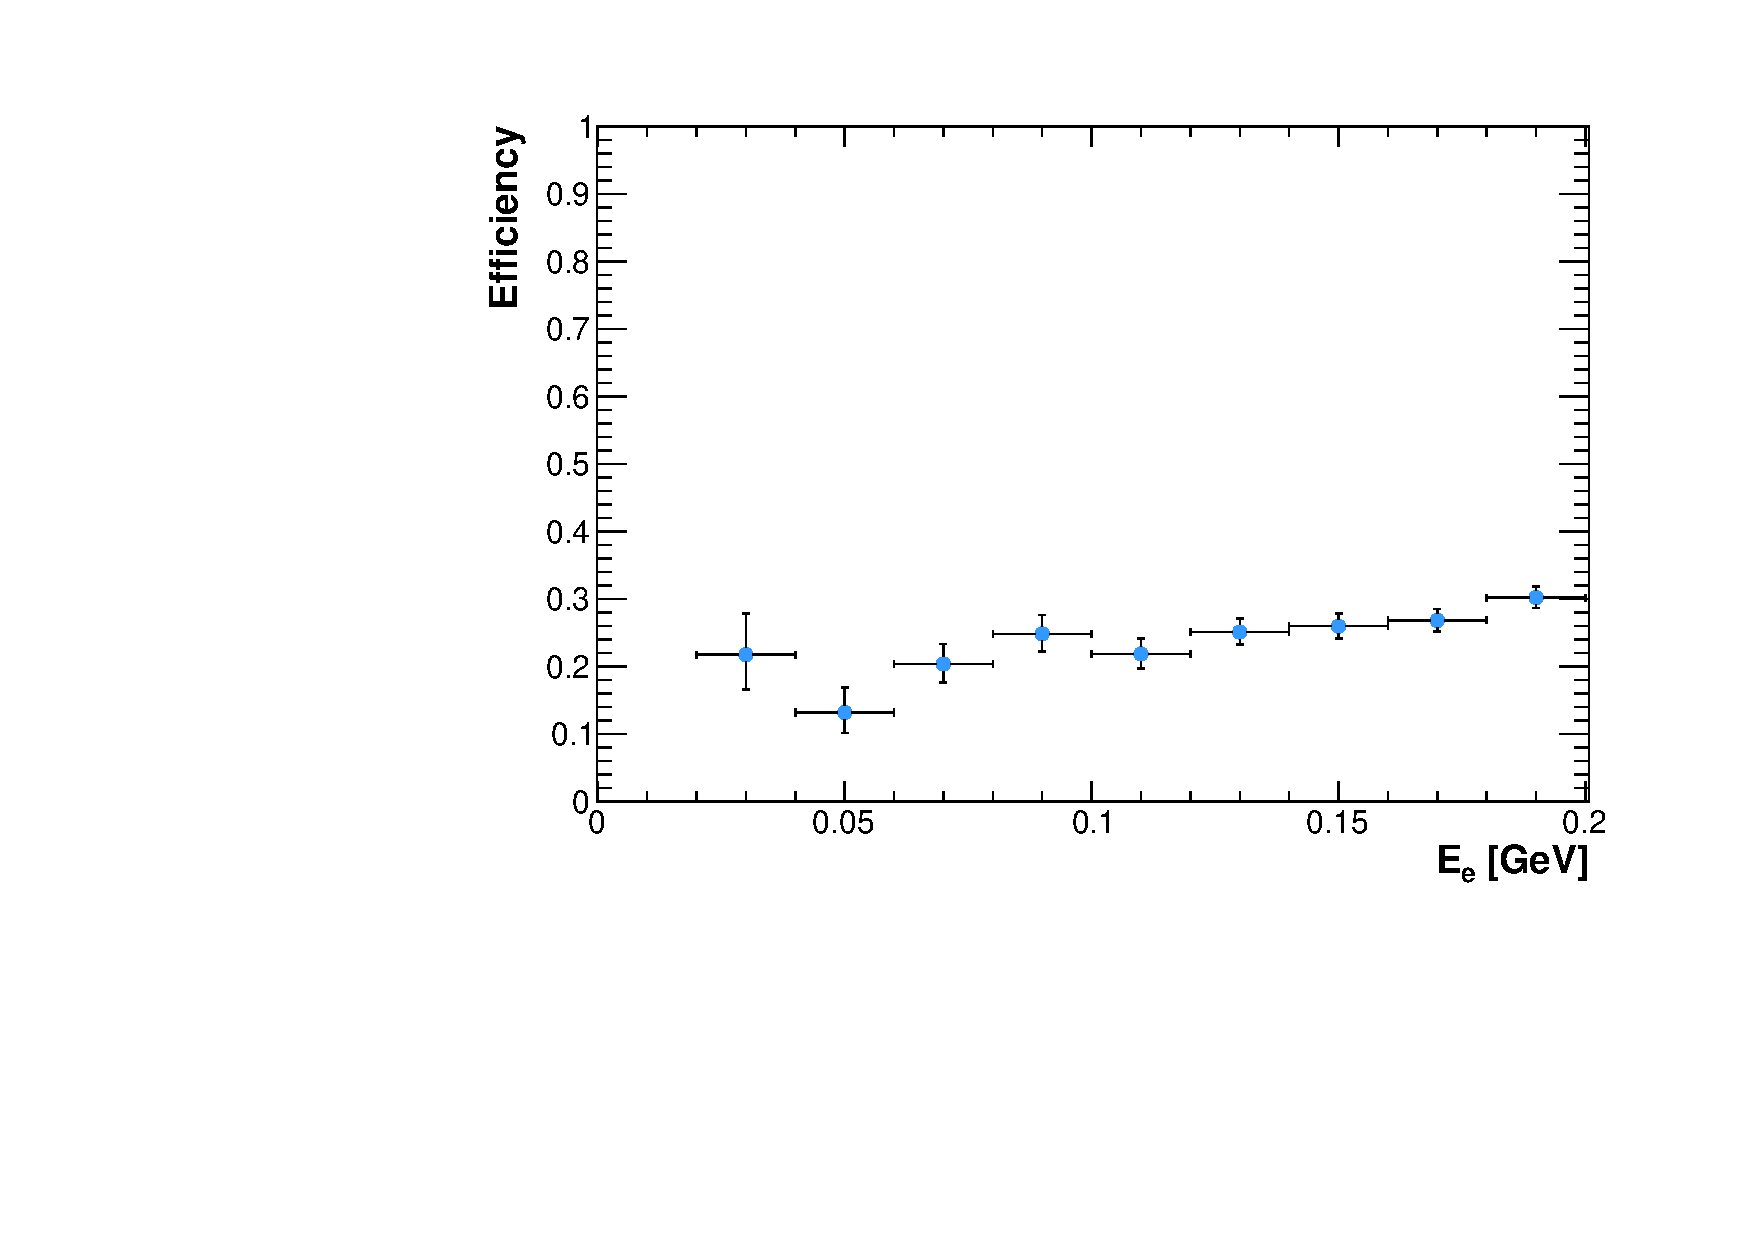
\includegraphics[width=\linewidth]{figures/electron_eff.pdf}
    \caption{Electron reconstruction efficiency} 
  \end{subfigure}
  \caption{Proton (left, in red) and electron (right, in blue) reconstruction efficiency for simulated $\nu_{e}$ CC$0\pi$-Np events. In our sample of generated $\nu_{e}$ CC$0\pi$-Np events we require at least one proton above 40~MeV and at least an above 20~MeV.}
  \label{fig:kin_eff}
\end{figure}


The selection efficiency $\epsilon$ is defined as:
\begin{equation}
\epsilon = \frac{\mathrm{N.~of~selected~CC0}\pi\mathrm{{\text -}Np~events}}{\mathrm{N.~of~generated~CC0}\pi\mathrm{{\text -}Np~events}},
\end{equation}
where each selected event must pass the optical selection and satisfy the topology requirement. A minimum quality of the selected event is also ensured requiring (1) at least 5 hits in the collection plane associated to a shower-like object, (2) at least 5 hits in the collection plane associated to a track-like object, and (3) at least one hit in every plane.
The start and end point of each track-like object and the start point of each shower-like object must also lie within the fiducial volume to ensure that the event is fully contained.

The purity of the sample is defined as:
\begin{equation}
\epsilon = \frac{\mathrm{N.~of~selected~CC0}\pi\mathrm{{\text -}Np~events}}{\mathrm{N.~of~selected~events}},
\end{equation}
and it has been measured running the selection algorithm on a complete sample of neutrino events (not only $\nu_{e}$ interactions), weighted accordingly to the Booster Neutrino Beam (BNB) flux. In this sample every event will have at least one neutrino interacting in the cryostat volume and triggering the detector, plus all the cosmic rays hitting the detector in the same readout window. In the data, however, this is not always true, since the detector can be triggered also by a cosmic ray producing a flash in the optical system during the beam window, without necessarily having a neutrino interaction. In order to estimate this background component, defined as \emph{in-time cosmic rays}, we have used the data EXT sample, which was collected using the standard detector trigger, but with the neutrino beam off.

Figure \ref{fig:effpurity} shows the efficiency as a function of the true neutrino energy and the purity as a function of the reconstructed energy. The energy reconstruction procedure is described in section \ref{sec:energyreco}.
As expected, the efficiency (purity) is proportional to the neutrino energy (reconstructed energy), since high-energy events correspond in general to a larger number of hits in the TPC and the Pandora framework reconstruction performances are proportional to the number of reconstructed hits 
\cite{pandora2}. 

\begin{figure}
  \begin{subfigure}{0.48\textwidth}
    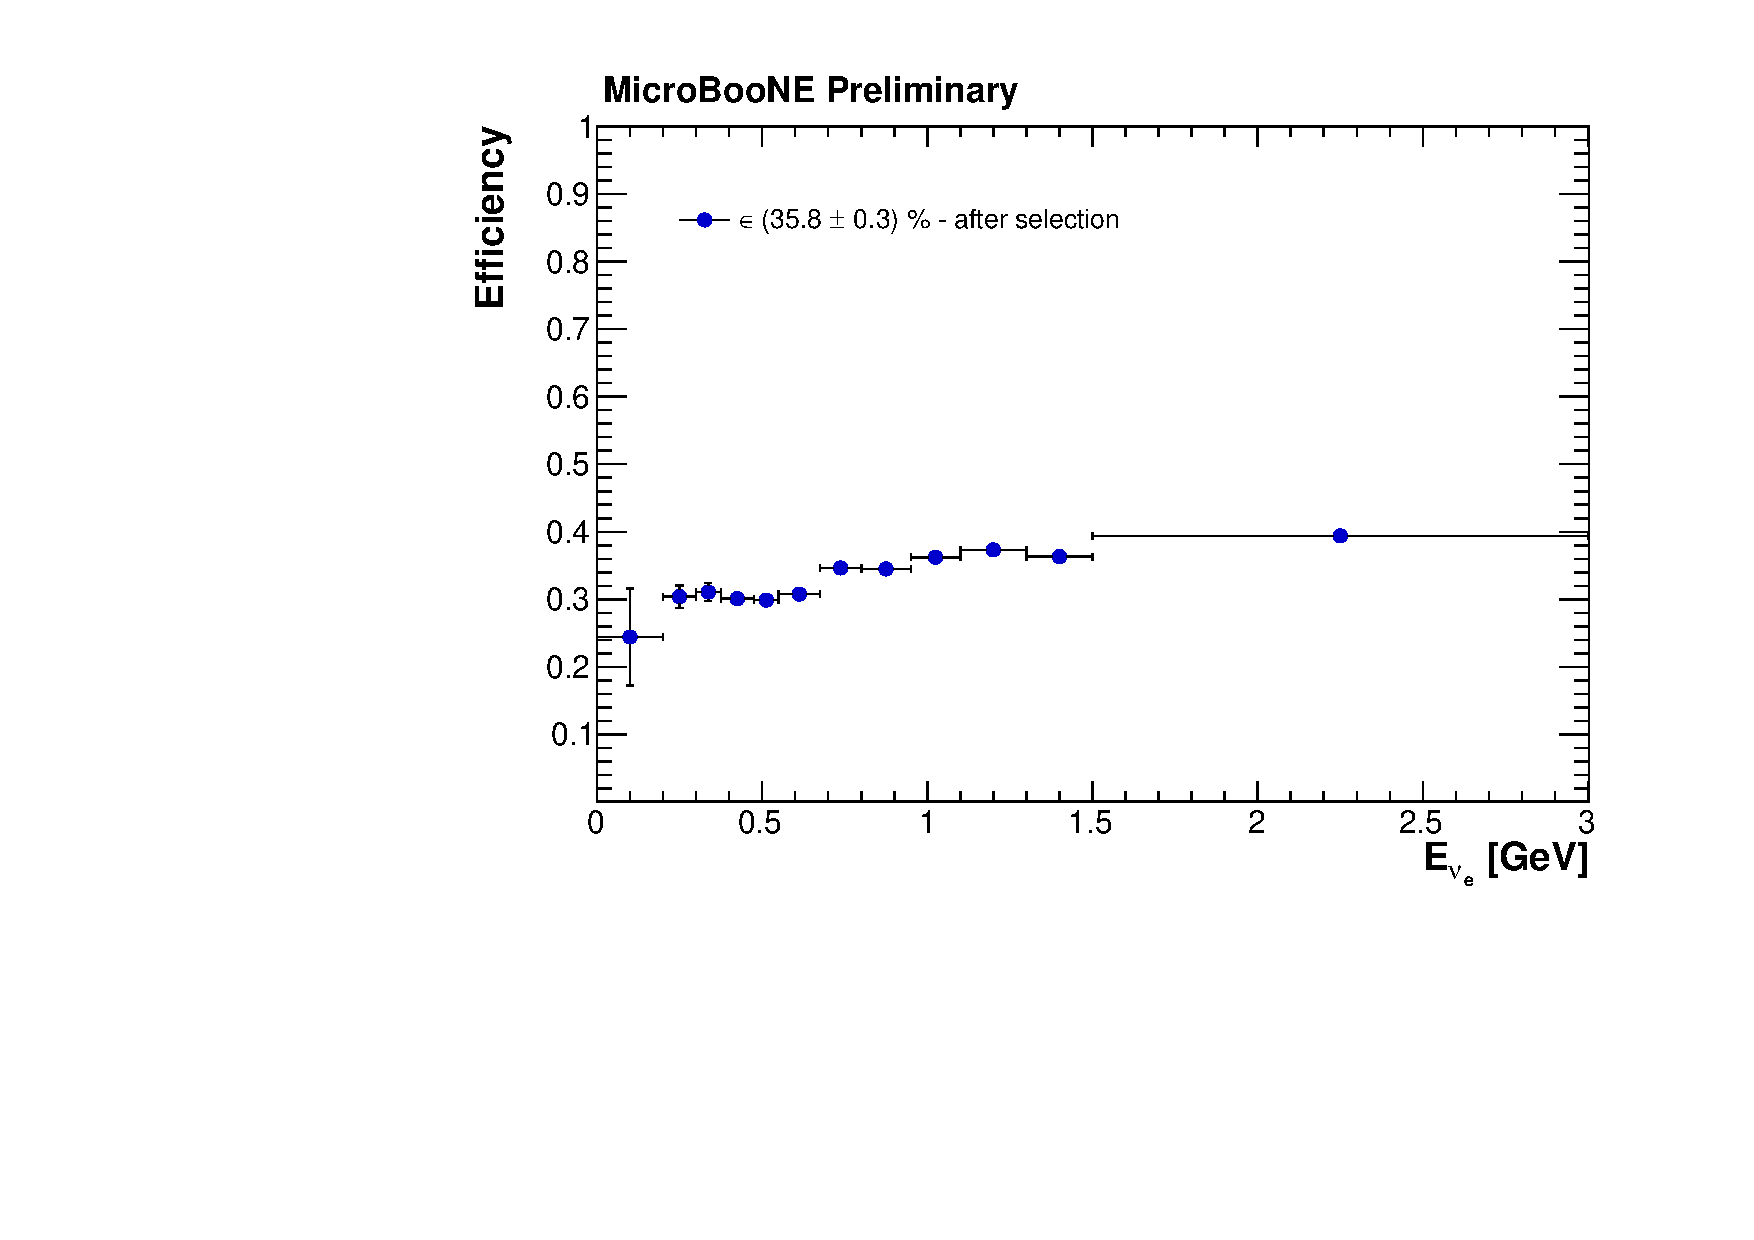
\includegraphics[width=\linewidth]{figures/eff.pdf}
    \caption{Efficiency} 
  \end{subfigure}
    \begin{subfigure}{0.48\textwidth}
    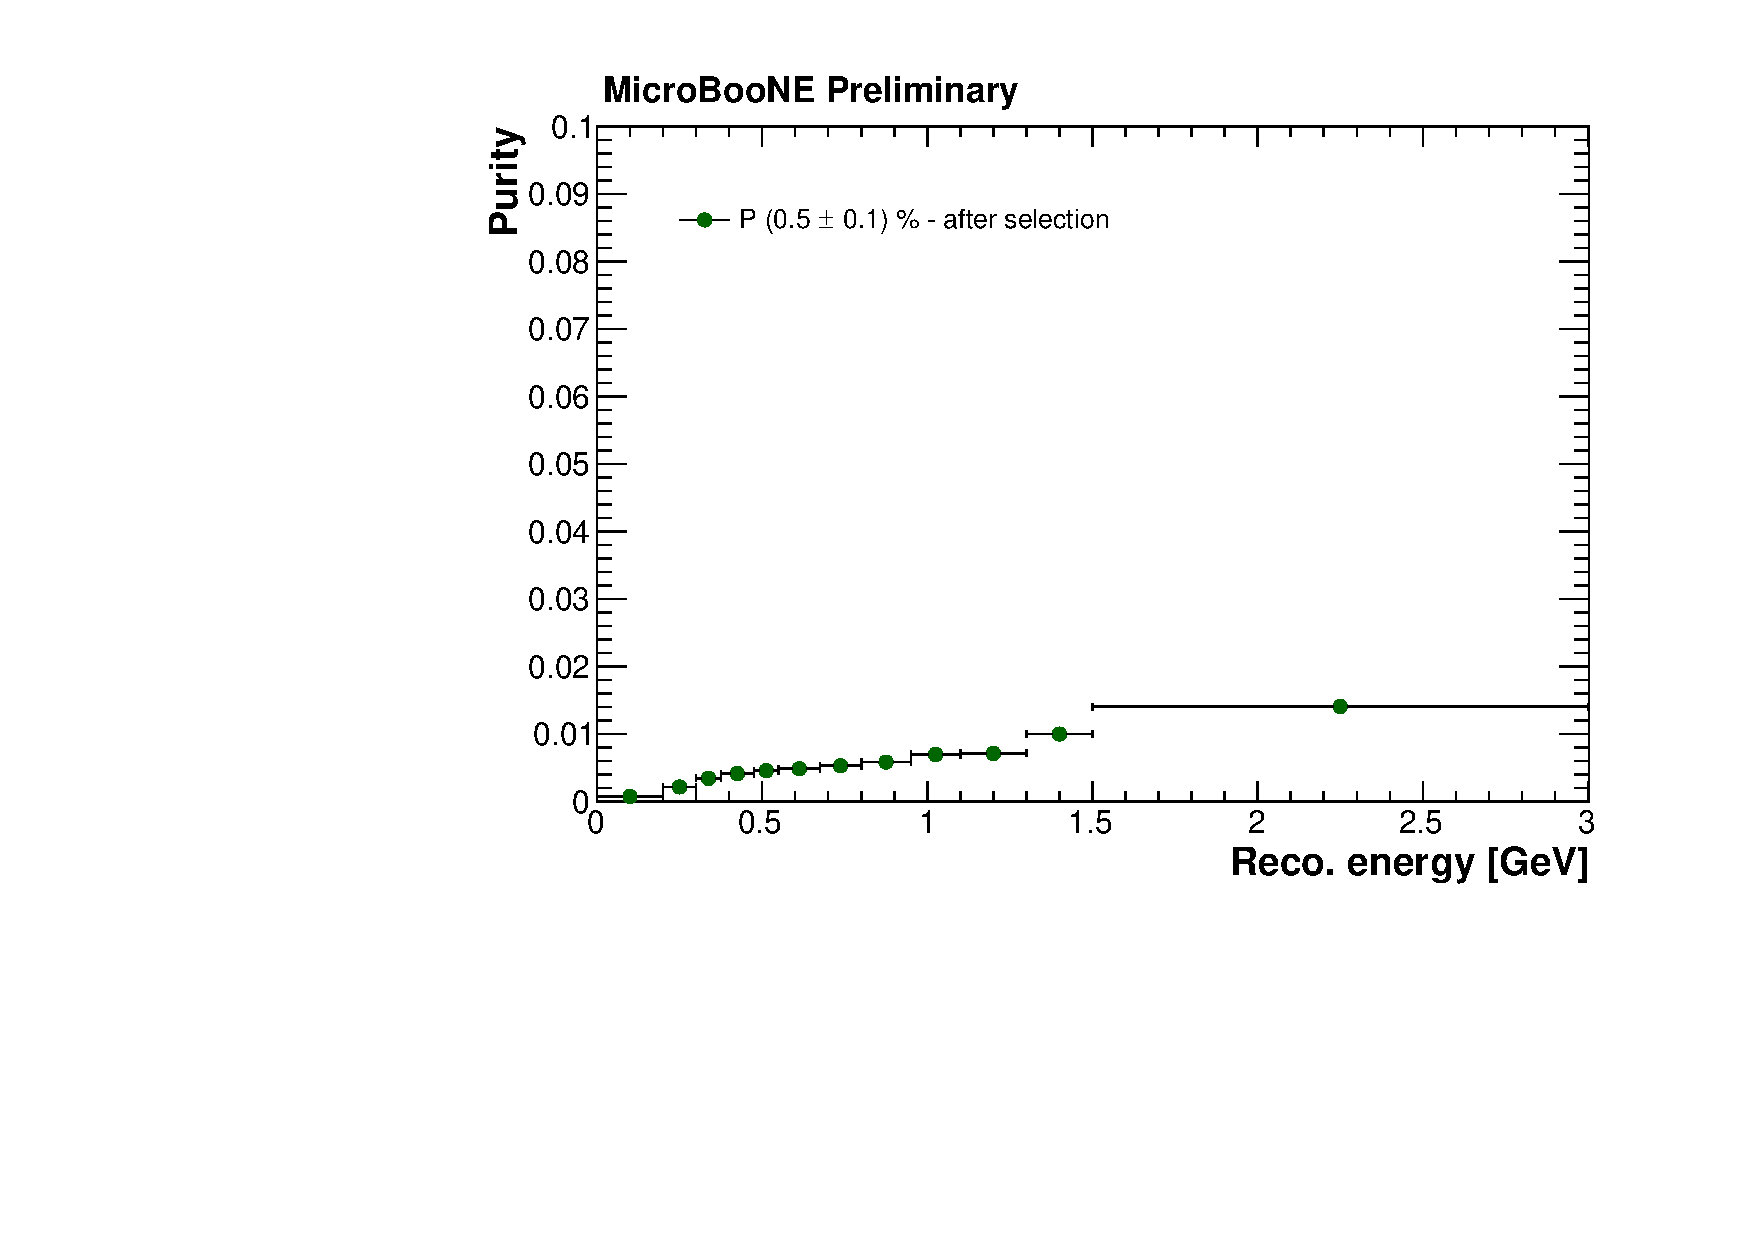
\includegraphics[width=\linewidth]{figures/purity.pdf}
    \caption{Purity} 
  \end{subfigure}
  \caption{Left: $\nu_{e}$ CC$0\pi$-Np reconstruction efficiency as a function of the true $\nu_{e}$ energy. Right: $\nu_{e}$ CC$0\pi$-Np purity as a function of the reconstructed energy.}
  \label{fig:effpurity}
\end{figure}

In order to understand the different background components, we divided our sample of selected events into further 8 categories:
\begin{description}
\item[Beam intrinsic $\nu_{e}$ CC$0\pi$-Np] charged-current $\nu_{e}$ neutrino interaction with no pions in the final state and at least one proton (N > 1).
\item[Beam intrinsic $\nu_{e}$ CC] charged-current $\nu_{e}$ neutrino interaction that is not in the $\nu_{e}$ CC$0\pi$-Np channel.
\item[Beam intrinsic $\nu_{\mu}$] charged-current $\nu_{\mu}$ neutrino interaction.
\item[Beam intrinsic NC] neutral current neutrino interaction (both $\nu_{\mu}$ and $\nu_{e}$).
\item[Dirt] the neutrino interacts outside the TPC, but one or more final-state particles produce a neutrino candidate inside in the fiducial volume.
\item[Cosmic] there is a neutrino interaction in the event, but the cosmic-ray interaction happening during the same drift time is selected instead.
\item[Cosmic in-time] there is no neutrino interaction in the event and a cosmic-ray interaction happening inside the beam gate time window is selected. It corresponds to the data EXT sample.
\item[Cosmic contaminated] the neutrino interaction candidate contains at least a track or a shower generated by a cosmic ray.
\end{description}


Table \ref{tab:result} shows a summary of the selection algorithm results, with the corresponding number of events for each category. The numbers correspond to an exposure of the MicroBooNE detector of \num{4.84e19} protons on target (POT), which is the amount of data available in the open sample.

\begin{table}[htbp]
   \centering
   \begin{tabular}{llrrrrr}
     \toprule
     Category & \phantom{a} & Generated & \phantom{a} & Selected & \phantom{a} & Efficiency \\
     \midrule

     $\nu_{e}$ CC0$\pi$-Np       & & 34.8     & & 14.3   & & 41.1\%\\
     $\nu_{e}$ CC                & & 35.7     & & 13.2   & & 37.0\%\\
     Beam intrinsic $\nu_{\mu}$  & & 11337.4  & & 918.3  & & 8.1\%\\
     Beam intrinsic NC           & & 3633.9   & & 342.2  & & 9.4\%\\
     Dirt                        & & 2609.5   & & 37.1   & & 1.4\%\\
     Cosmic in-time              & & 135377.2 & & 1151.6 & & 0.9\%\\
     Cosmic contaminated         & & -        & & 260.7  & & -\\
     Cosmic                      & & -        & & 233.3  & & -\\

     \bottomrule
   \end{tabular}
   \caption{Summary of the selection algorithm results, showing the contribution of each event category, for a MicroBooNE exposure of \num{4.84e19} POT.}\label{tab:result}
\end{table}


\subsection{CC \texorpdfstring{$\nu_{\mu}$}{numu} Event Rejection}\label{sec:numu}
The module \texttt{UBXSec} \cite{ubxsec} looks for charged-current $\nu_{\mu}$ candidates and it also helps reject cosmic-induced background events.  Figure \ref{fig:spectrum} shows the reconstructed energy spectrum obtained vetoing the events that \texttt{UBXSec} flagged as CC $\nu_{\mu}$ candidates or cosmic-induced background. The reconstructed energy has been measured with the procedure described in Section \ref{sec:energyreco}, after reclassifying the reconstructed Pandora objects as described in Section \ref{sec:reclass}. The ratio between the number of data events and the number of Monte Carlo events (POT normalized) is 1 and the low value of the $\chi^{2} / \mathrm{n.d.f.}$ (1.06) shows that the two distributions agree also in shape. This plot also shows that our selection procedure has similar performances in data and Monte Carlo and that there is no evident bias in the energy reconstruction.

\begin{figure}[htbp]
\centering
  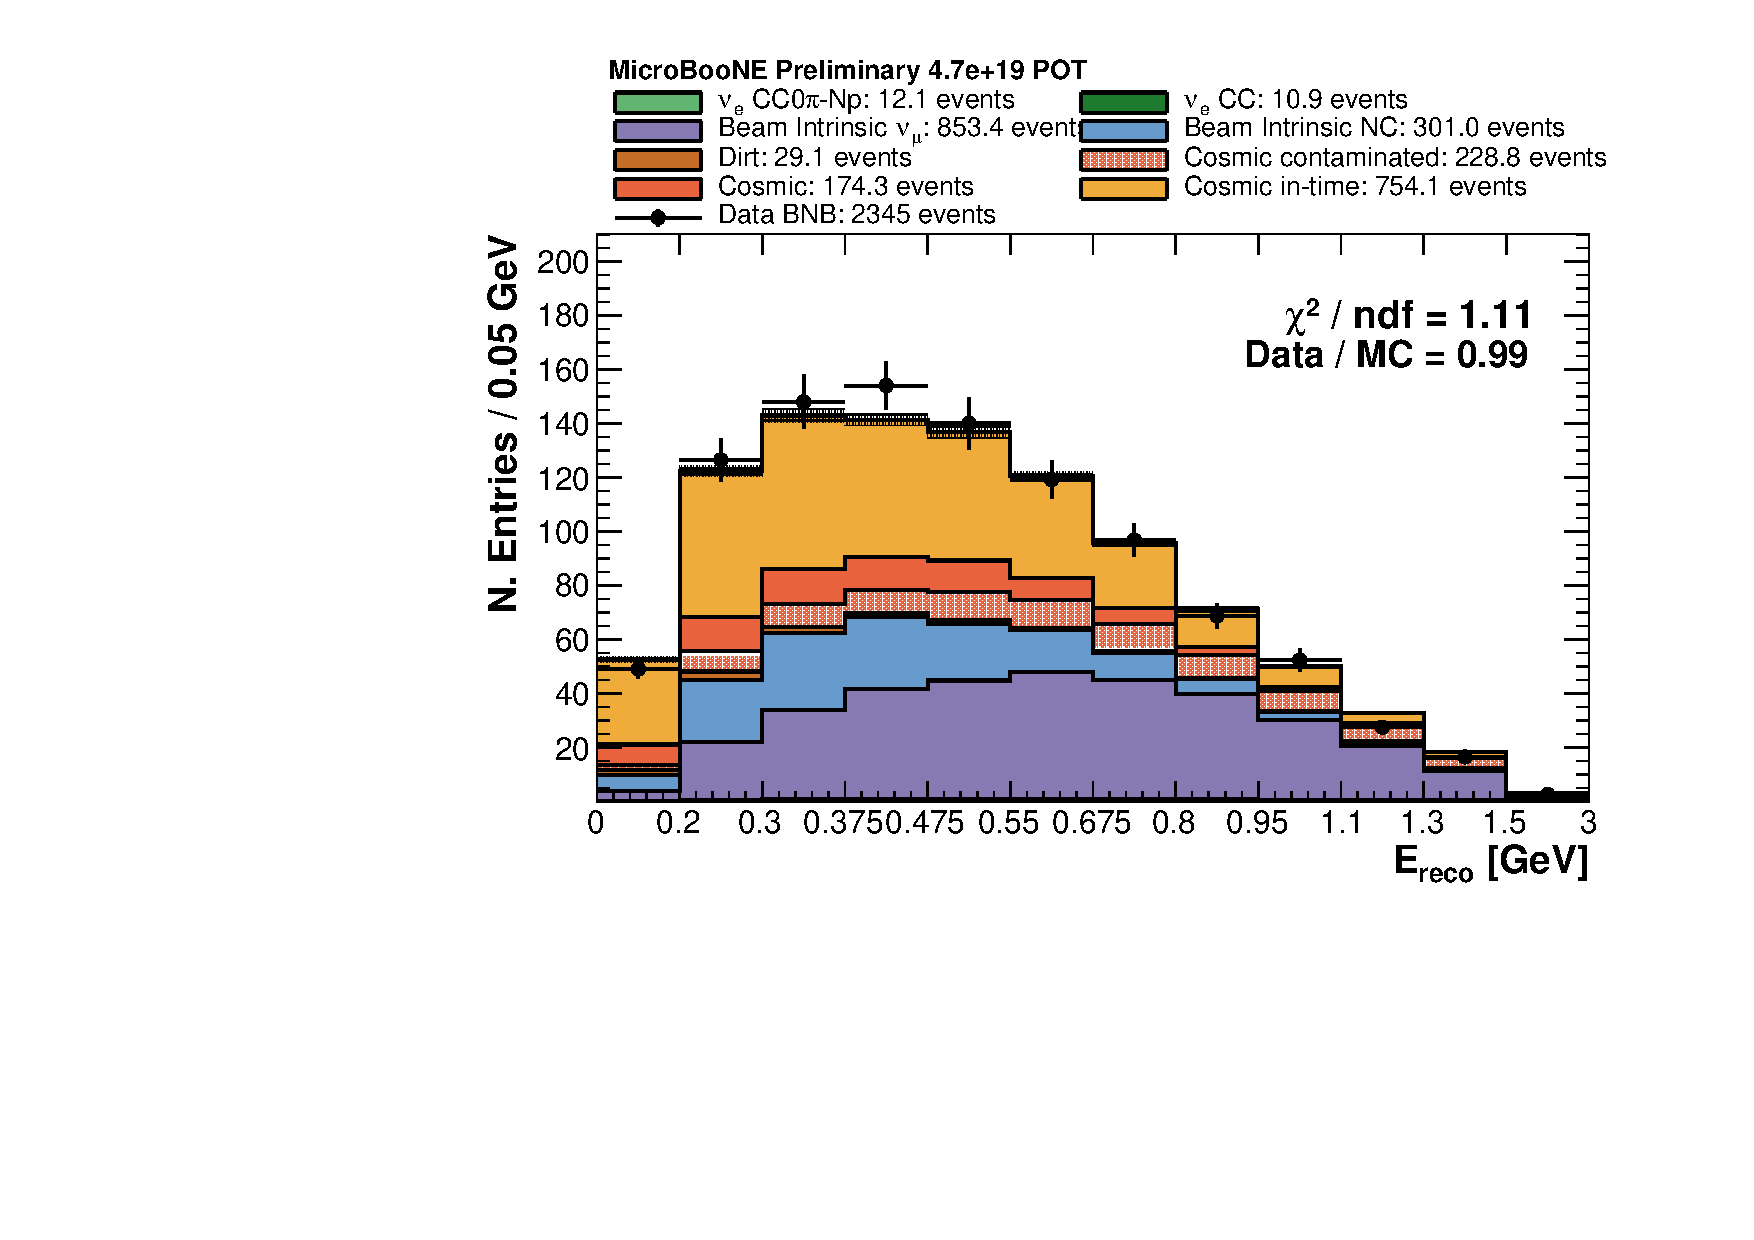
\includegraphics[width=0.65\linewidth]{figures/h_fixed_energy.pdf}
  \caption{Reconstructed energy spectrum after the event selection algorithm and the veto of the events selected by the \texttt{UBXSec} module. The histograms of the event categories are stacked.}
  \label{fig:spectrum}
\end{figure}



\subsection{Track-like/Shower-like object reclassification}\label{sec:reclass}
\subsubsection{Classifier disagreement}
An object reconstructed by the Pandora framework in the TPC can be of two distinct types: track-like or shower-like. This assignment is performed directly by the Pandora framework using a Support Vector Machine. However, the scope of the framework is very broad and the object classification is not optimized on our topology. 
The classifier is trained on simulated events, using information from all the three wire planes and its performances are proportional to the number of reconstructed hits. As such, even a slight disagreement between the detector behavior and its simulation in any of the wire planes can have a strong impact on the classification of track-like or shower-like objects. 
Since our analysis heavily relies on the category of the reconstructed objects in its topology pre-selection, a good agreement between the classifier performances in data and Monte Carlo is essential.
Moreover, the energy reconstruction procedure is different for track-like and shower-like objects, as described in Section \ref{sec:energyreco}: an eventual classification disagreement will directly cause a disagreement in the reconstructed energy spectrum.


\begin{figure}[htbp]
\centering
  \begin{subfigure}{0.45\textwidth}
    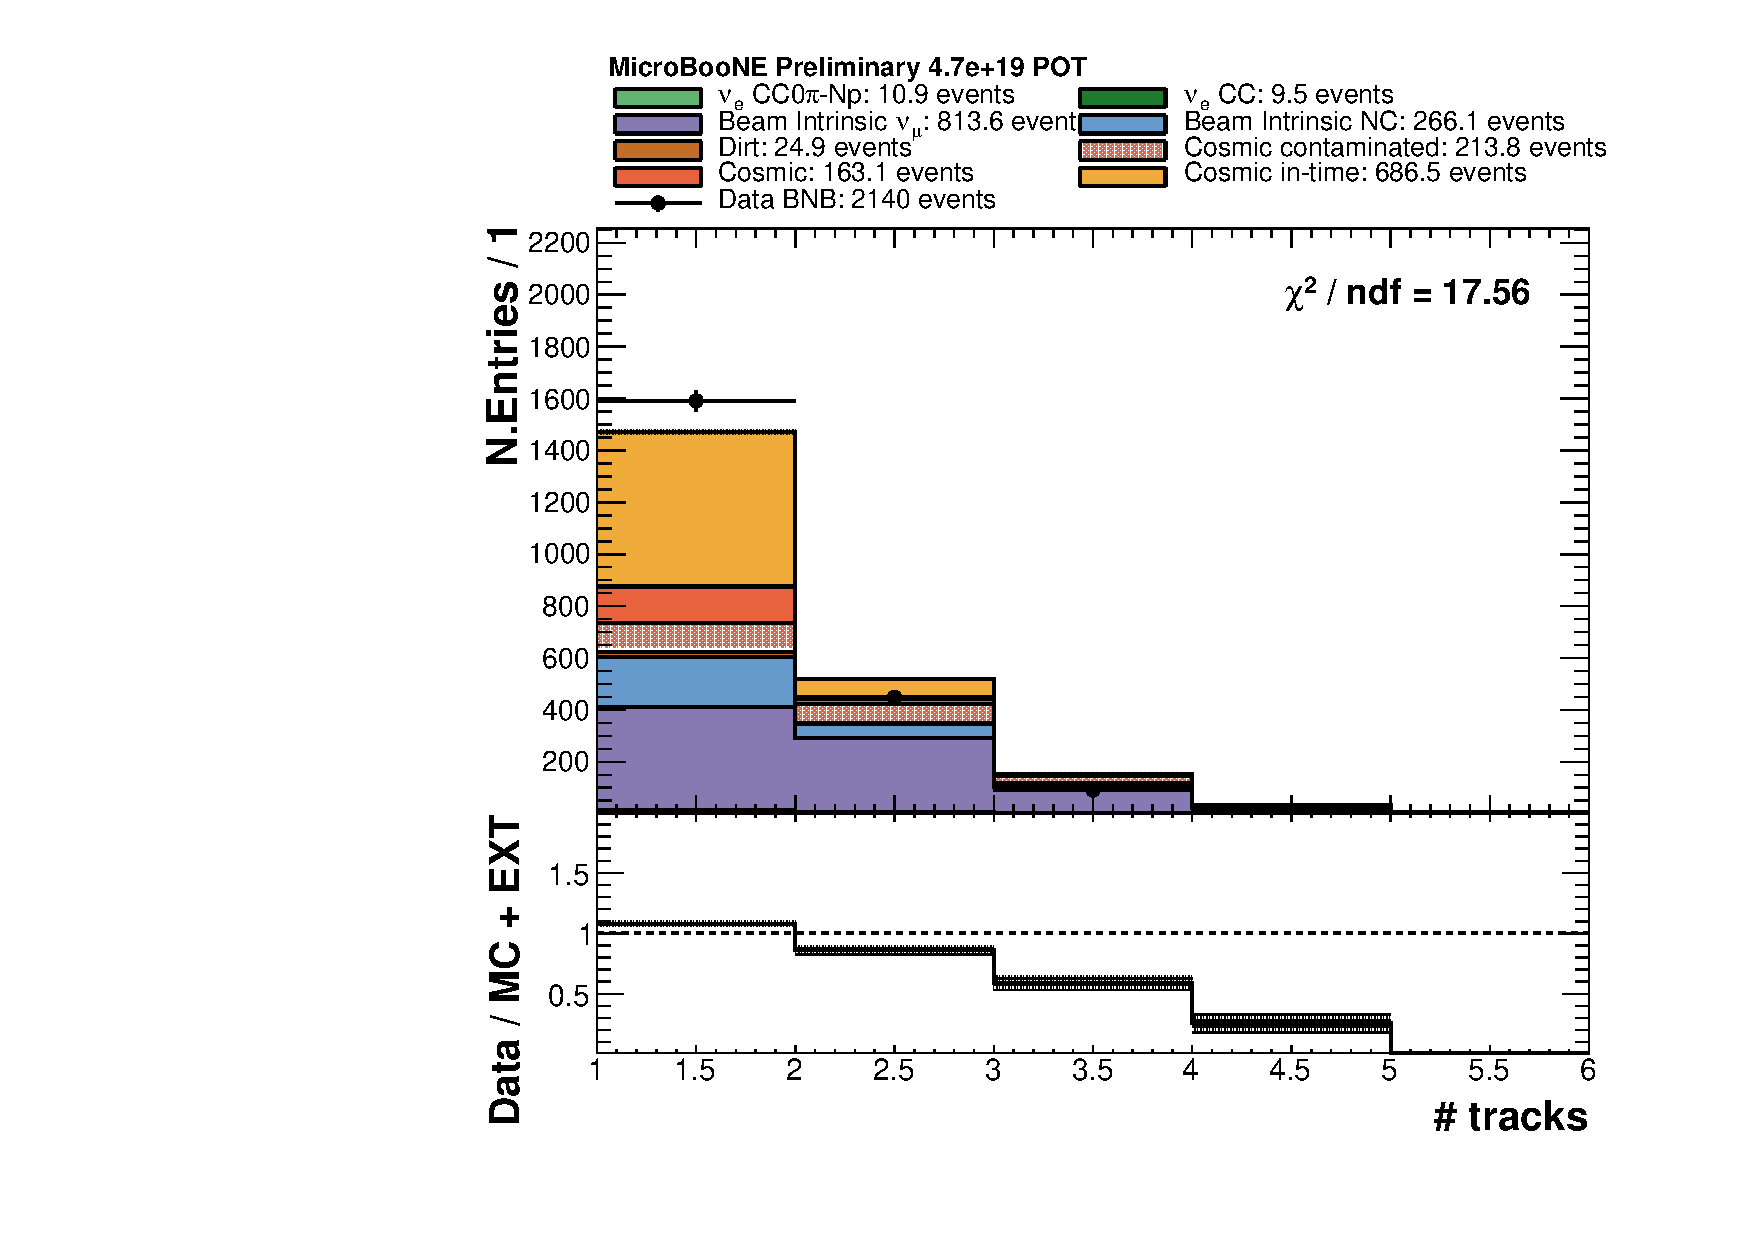
\includegraphics[width=\linewidth]{figures/h_n_tracks_before.pdf}
    \caption{Number of tracks.} 
  \end{subfigure}
    \begin{subfigure}{0.45\textwidth}
    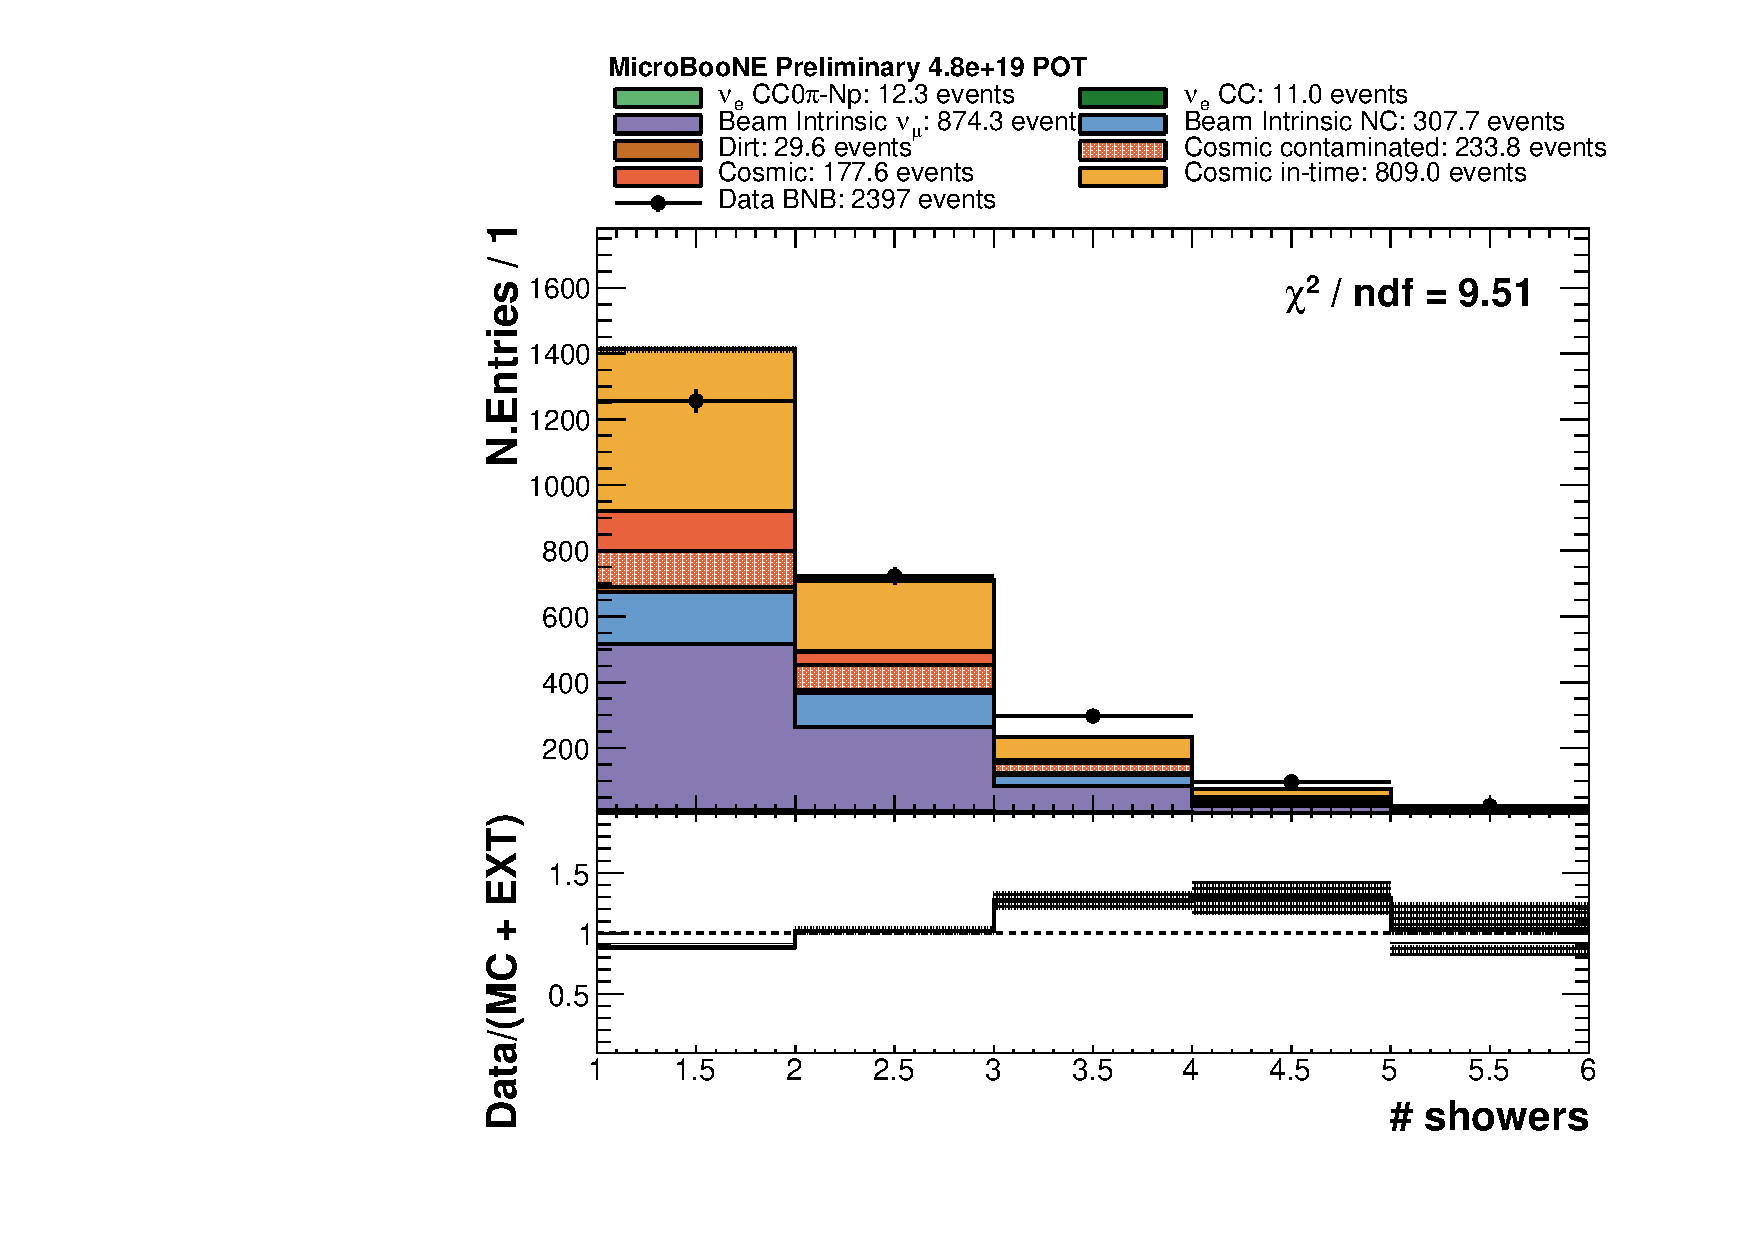
\includegraphics[width=\linewidth]{figures/h_n_showers_before.pdf}
    \caption{Number of showers.} 
  \end{subfigure}
  \caption{Number of tracks and number of showers per event before the reclassification procedure.}\label{fig:nshowers}
\end{figure}

The distributions of the number of track-like objects and of the number of shower-like objects in a selected event hint at a tendency of the classifier to select an object as shower-like more often in the data than in the simulation.

\begin{figure}[htbp]
\centering
  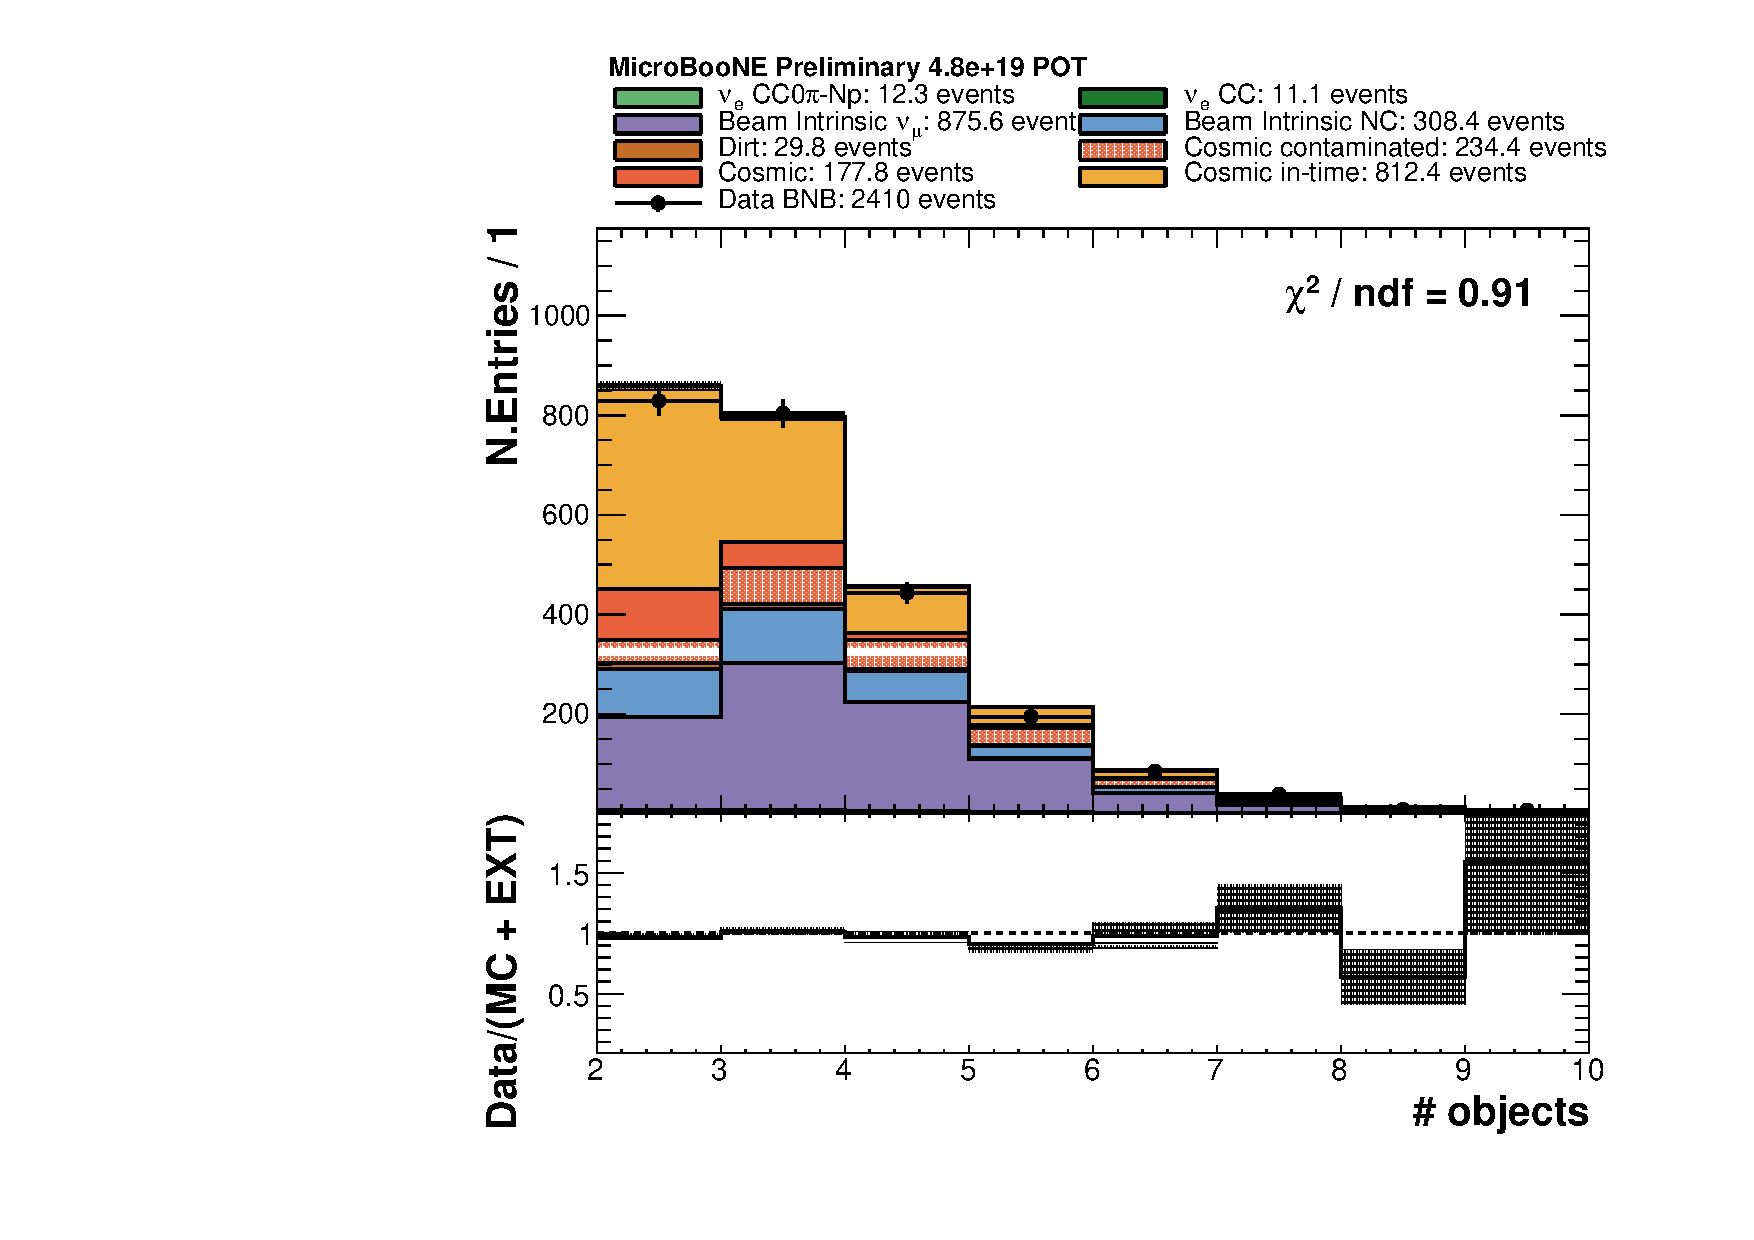
\includegraphics[width=0.65\linewidth]{figures/h_n_objects.pdf}
  \caption{Distribution of the total number of reconstructed objects per event.}
  \label{fig:nobjects}
\end{figure}

Figure \ref{fig:nshowers} shows the number of showers and the number of tracks per event in our selected sample after the optical and topological pre-selection. The ratio plot clearly indicates the presence of a bias: there are more events with a high number of reconstructed showers and more events with a low number of reconstructed tracks in the data than in the Monte Carlo. 

The distribution of the total number of reconstructed objects in Figure \ref{fig:nobjects} (regardless of their category) shows instead a very good agreement and no bias.


The simulation does not perfectly reflects the detector status: in particular, we measured the hit residuals of the track-like objects in the collection plane, defined as the distance between the reconstructed hit position in two dimensions (wire, time) and the reconstructed track trajectory. Figure \ref{fig:res} shows that the distribution of the mean of the residuals is peaked around zero as expected, both for data and Monte Carlo, while the standard deviation in the data is shifted towards higher values. 

\begin{figure}[htbp]
\centering
  \begin{subfigure}{0.45\textwidth}
    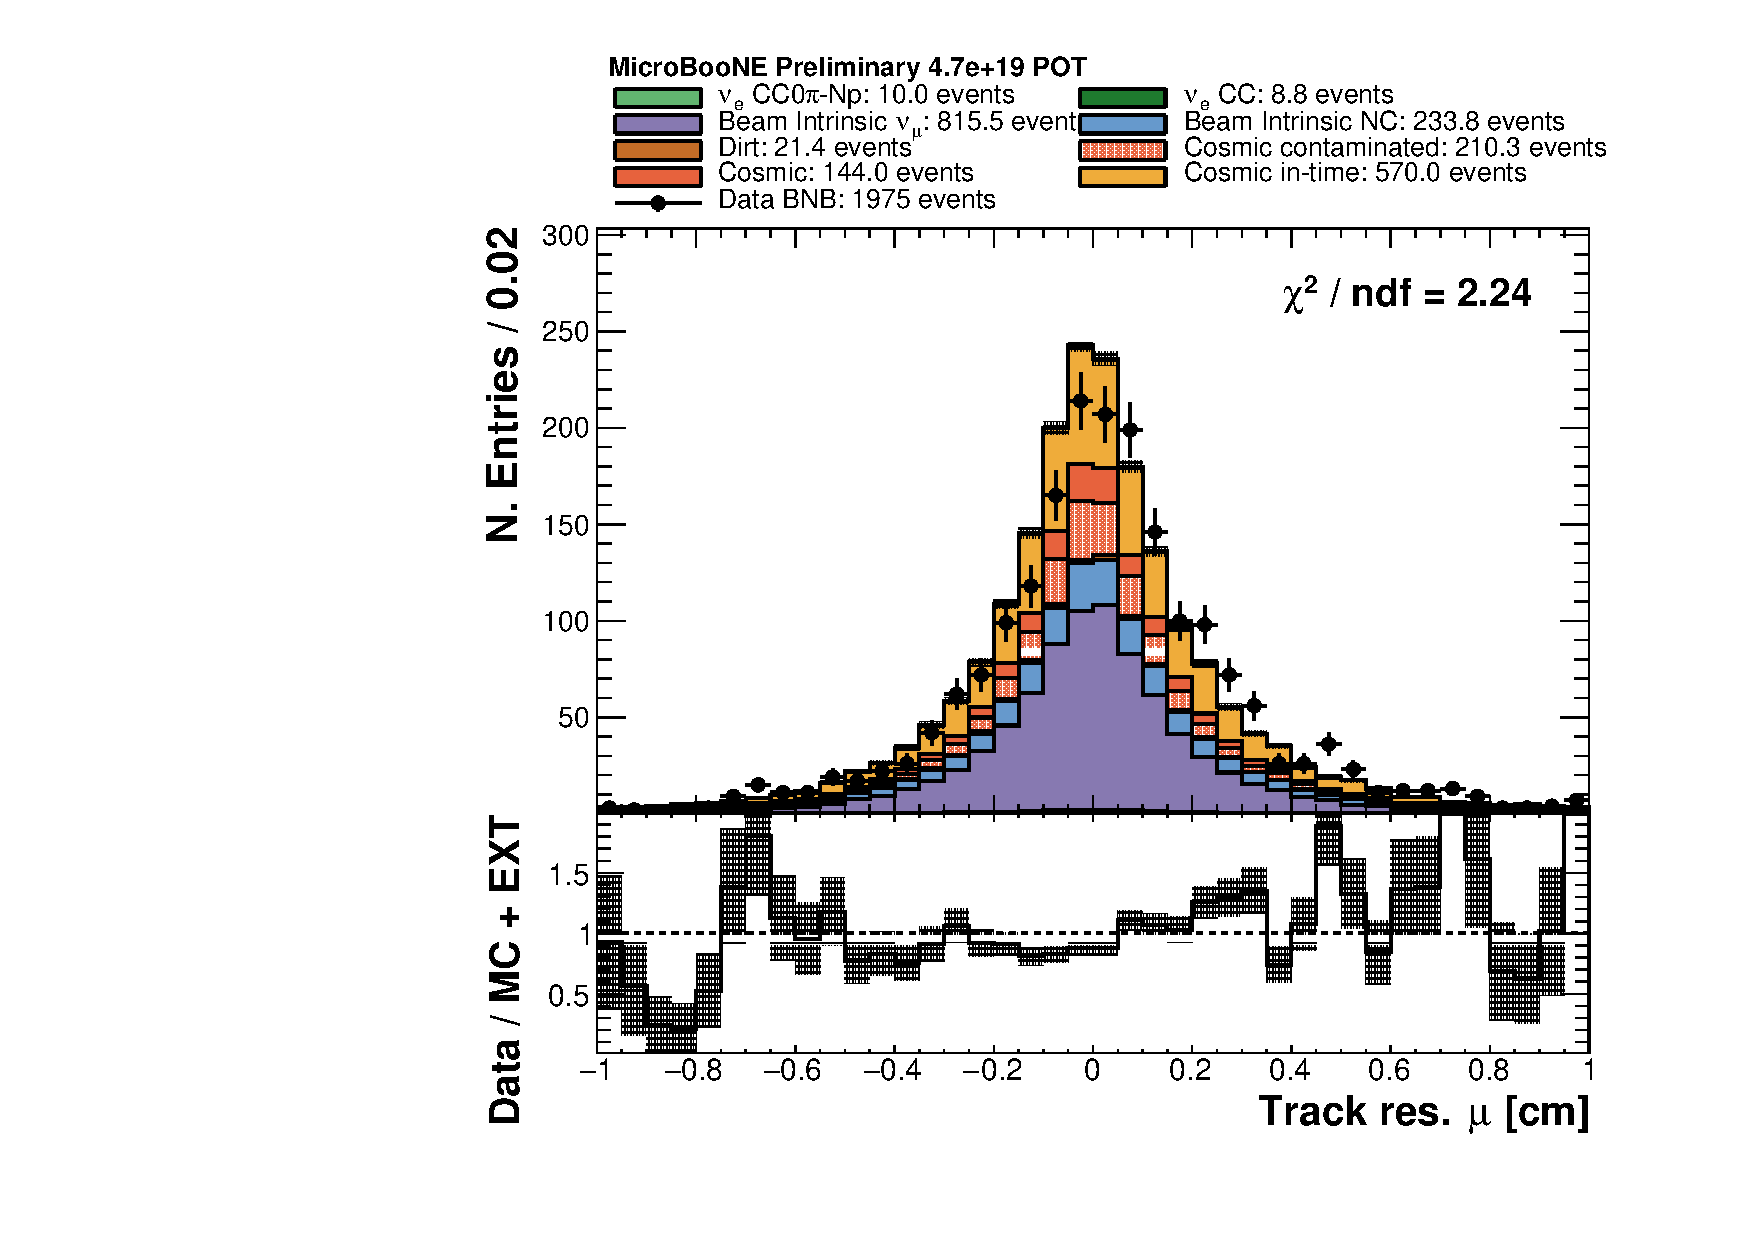
\includegraphics[width=\linewidth]{figures/h_track_res_mean.pdf}
    \caption{Track residual mean.} 
  \end{subfigure}
    \begin{subfigure}{0.45\textwidth}
    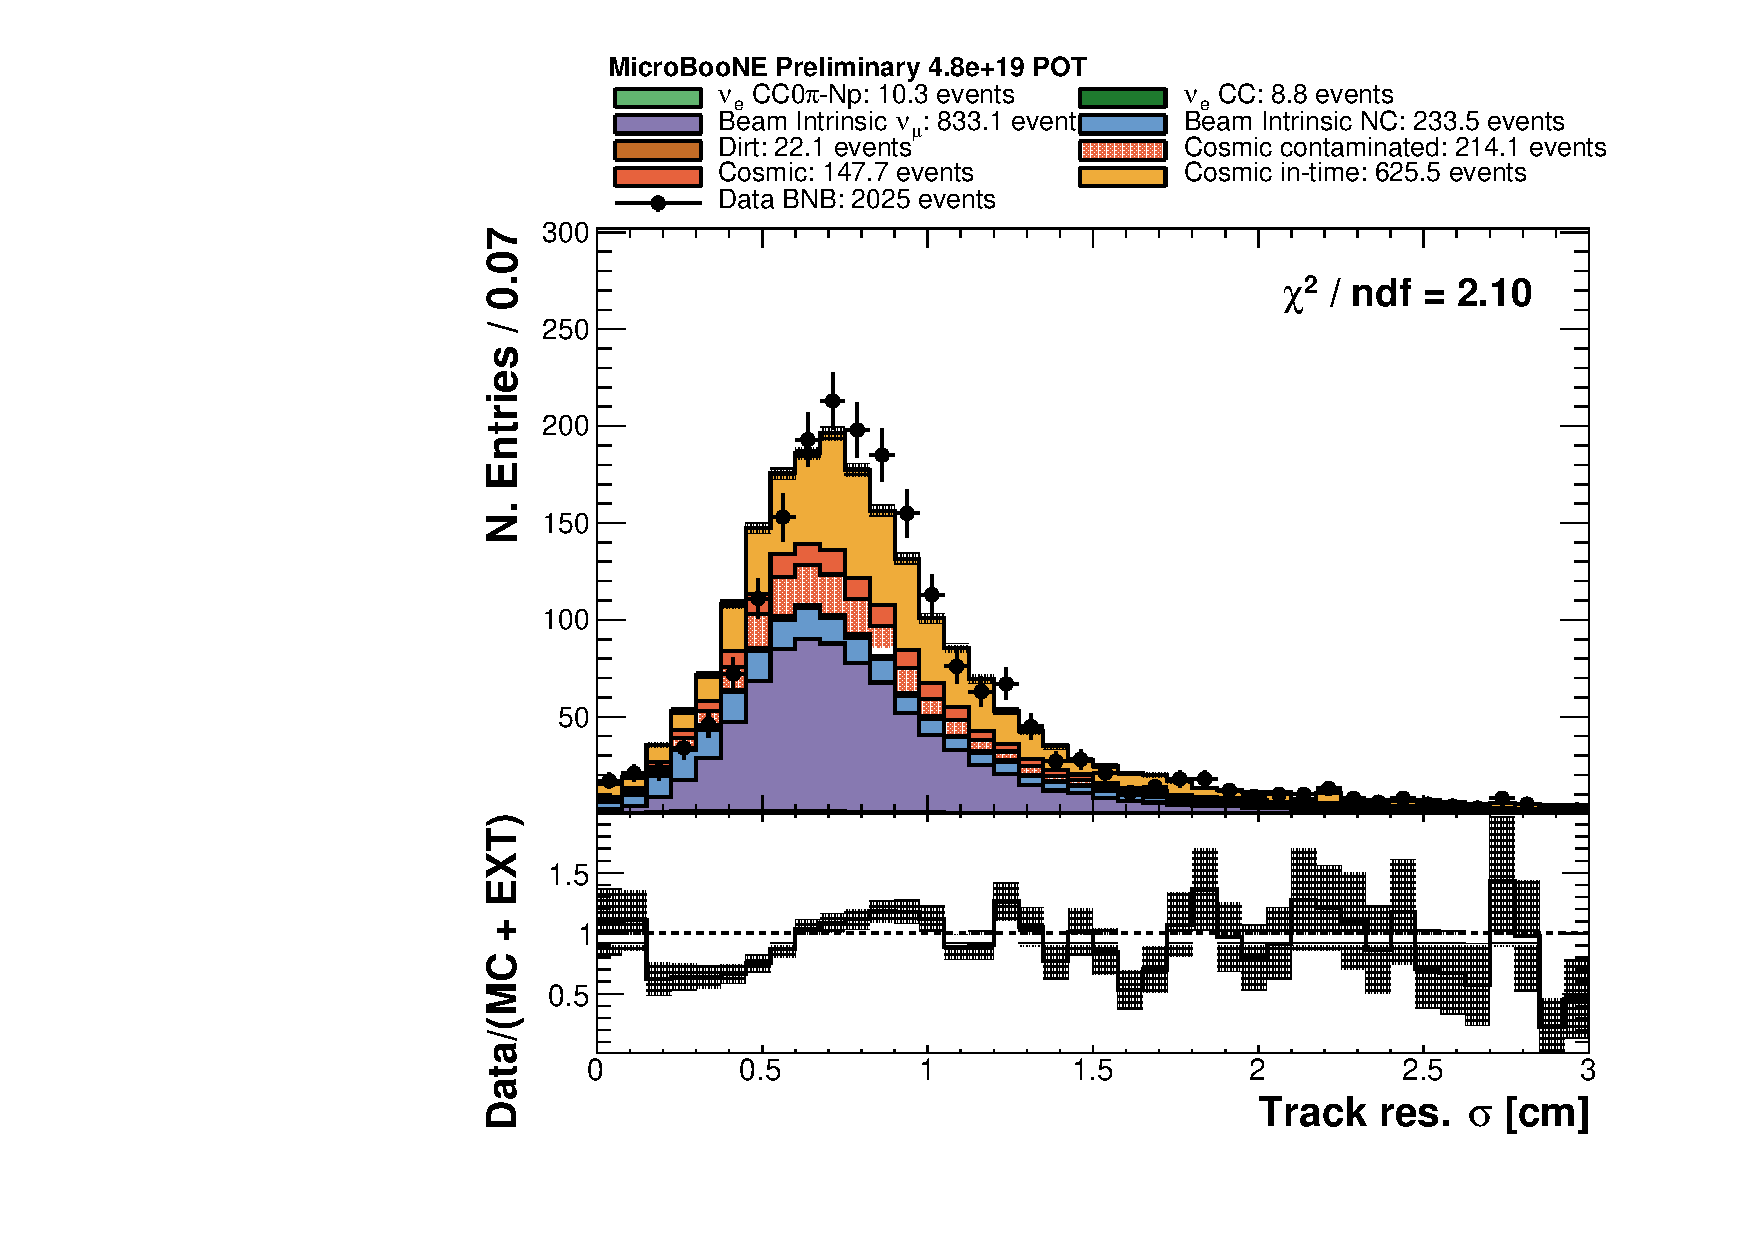
\includegraphics[width=\linewidth]{figures/h_track_res_std.pdf}
    \caption{Track residual standard deviation.} 
  \end{subfigure}
  \caption{Distribution of the mean and of the standard deviation of the track residuals.}\label{fig:res}
\end{figure}

The distribution of the principal component eigenvalue for track-like objects and shower-like objects also shows a disagreement: the data distributions are broader and the ratios have a decreasing slope, especially for high values (Figure \ref{fig:pca}).

\begin{figure}[htbp]
\centering
  \begin{subfigure}{0.45\textwidth}
    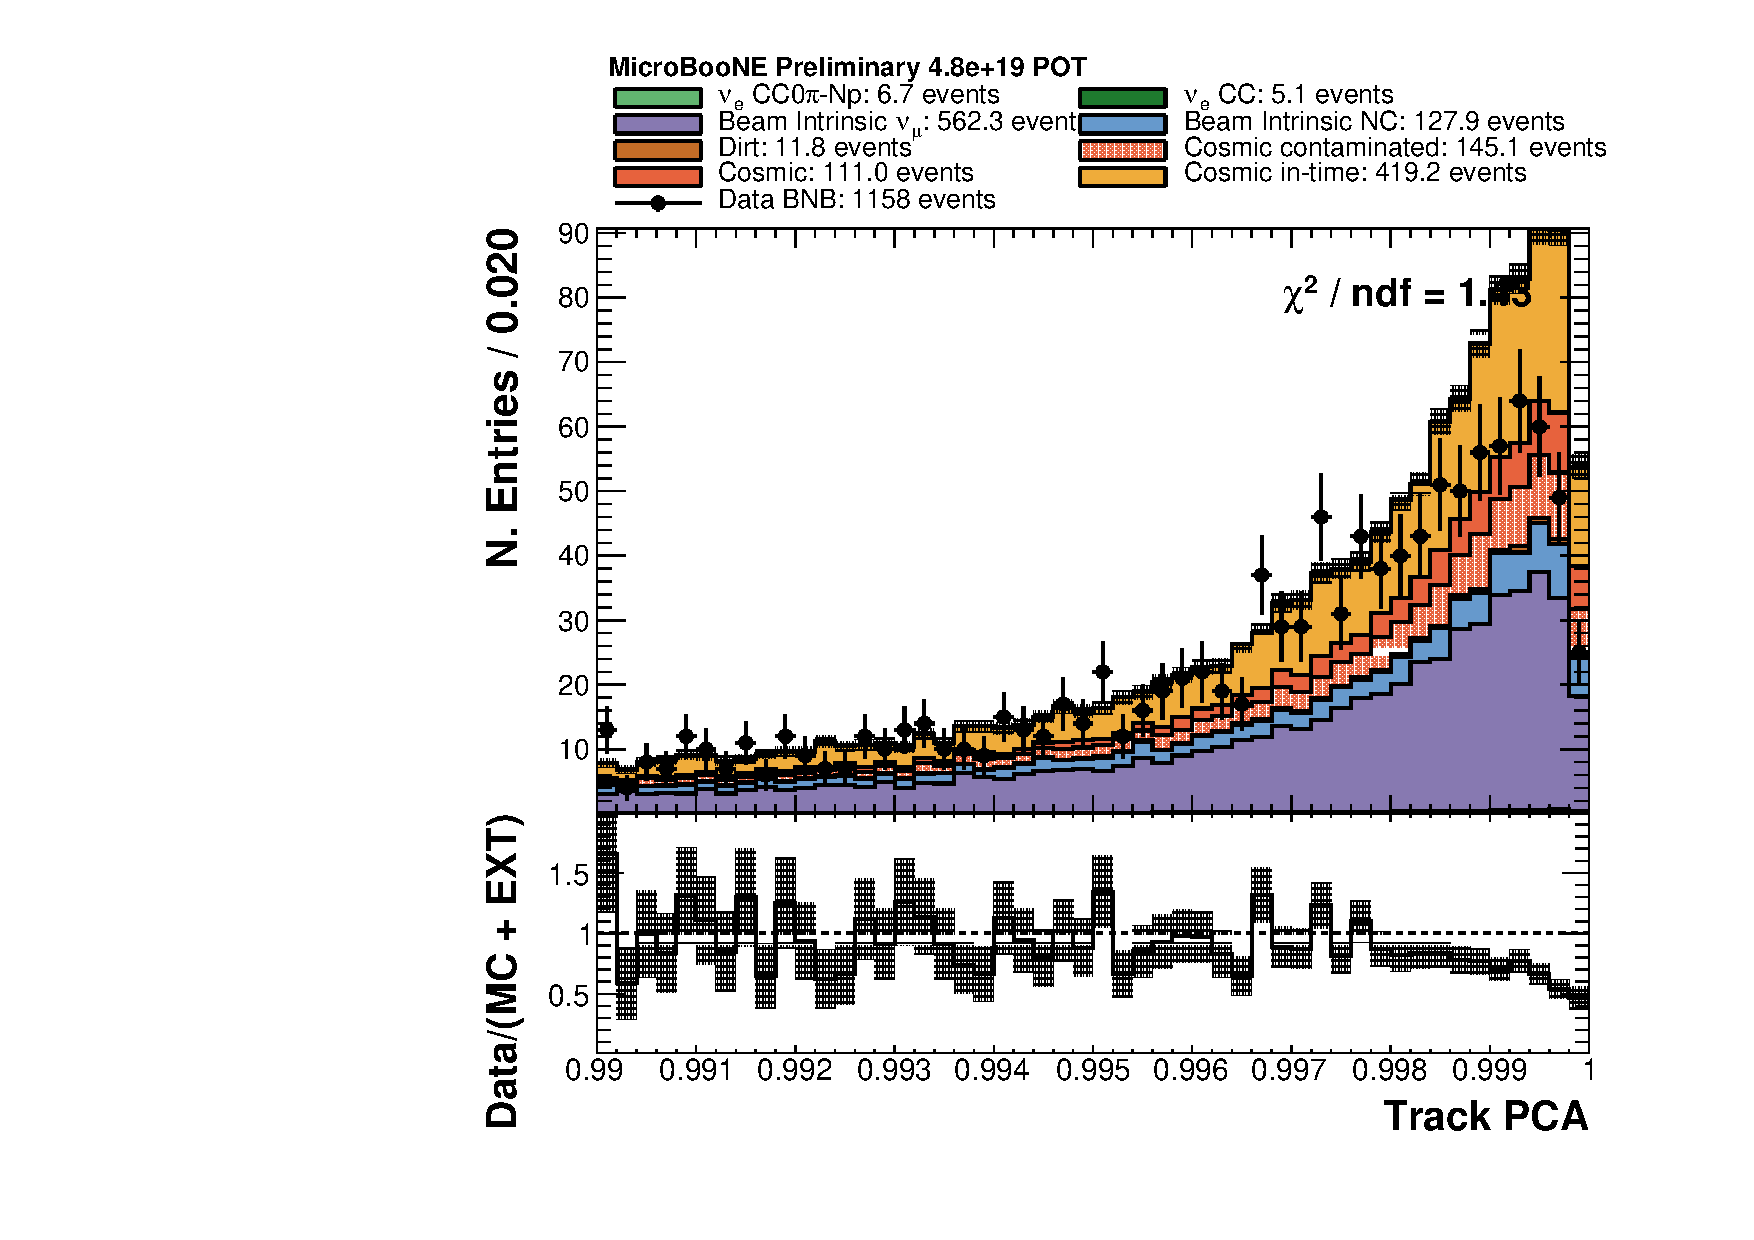
\includegraphics[width=\linewidth]{figures/h_track_pca.pdf}
    \caption{Track PCA eigenvalue.} 
  \end{subfigure}
    \begin{subfigure}{0.45\textwidth}
    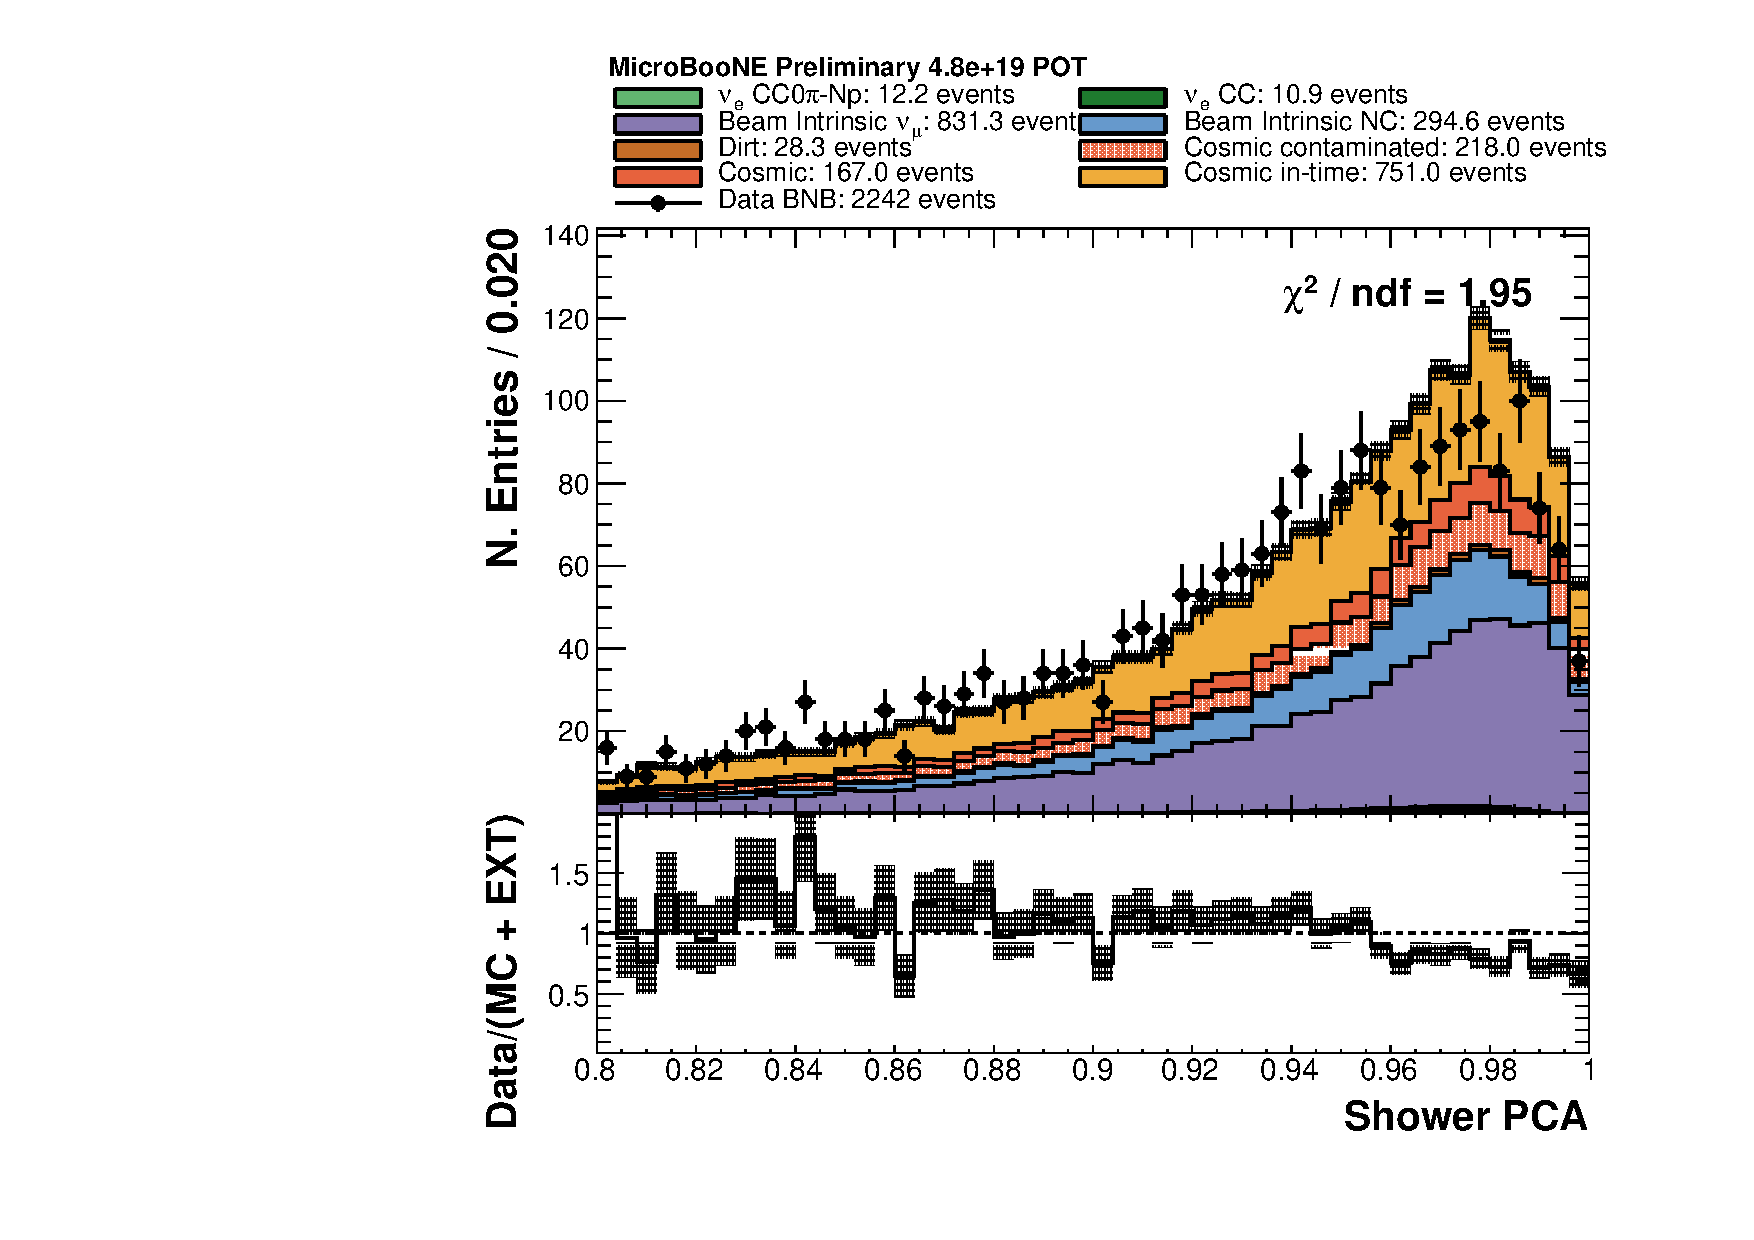
\includegraphics[width=\linewidth]{figures/h_shower_pca.pdf}
    \caption{Shower PCA eigenvalue.} 
  \end{subfigure}
  \caption{Principal Component first eigenvalue for reconstructed tracks and reconstructed showers.}\label{fig:pca}
\end{figure}

This evidence points towards a detector mis-modeling in the simulation: Figure \ref{fig:evdpandora} shows the Pandora data event display in one of the induction plane of a track objects that was reconstructed as a shower-like object. The presence of noise hits around the track created artifacts that induced the SVM to classify the object as a shower.

\begin{figure}[htbp]
\centering
  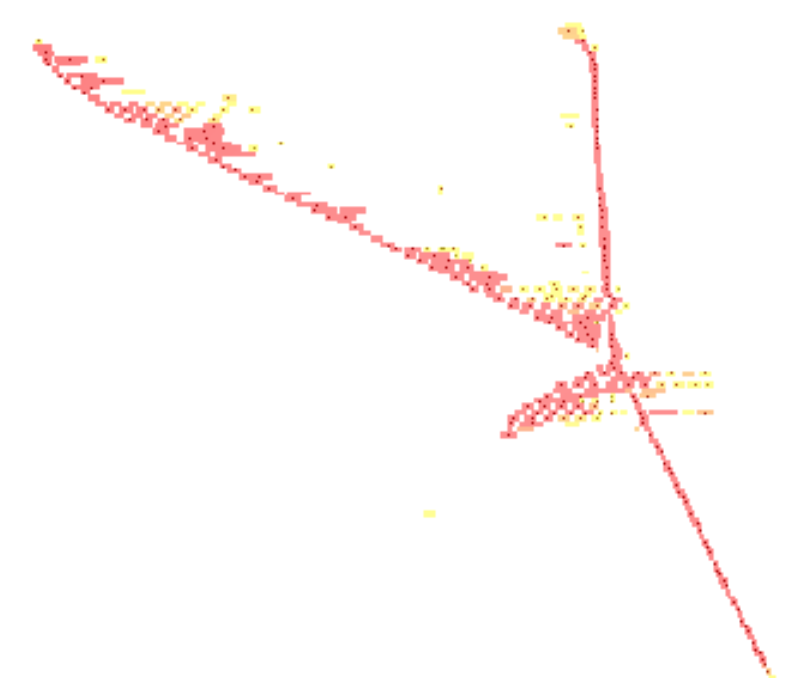
\includegraphics[width=0.45\linewidth]{figures/pandora.png}
  \caption{Pandora data event display in one of the induction plane of a track objects that was reconstructed as a shower-like object.}
  \label{fig:evdpandora}
\end{figure}

\subsubsection{Reclassification procedure}
In order to solve this discrepancy it is possible to reclassify the reconstructed objects exploiting the particular topology of our signal events. In particular, a well-reconstructed $\nu_{e}$ CC0$\pi$-Np event will have a reconstructed shower corresponding to the electron and N reconstructed tracks, where N is the number of protons above detection threshold. 

The Pandora reconstruction framework can split the electromagnetic shower in two or more objects: however, even if distinct, the showers will have in general a low angular separation. A small reconstructed shower-like object with a high angular separation from the most energetic one has a high probability to be in reality a mis-reconstructed proton track. Thus, we reclassify the shower-like objects based on the angular separation between each small shower-like object and the most-energetic shower: if the angle is larger than $15^{\circ}$, the shower-like object is reclassified as a track-like object.

Figure \ref{fig:showerangle} shows the proton reconstruction efficiency and purity as a function of the angular reclassification cut. The $15^{\circ}$ threshold is chosen because it maximizes the efficiency while keeping a reasonable reconstruction purity (above 70\%).

\begin{figure}[htbp]
\centering
  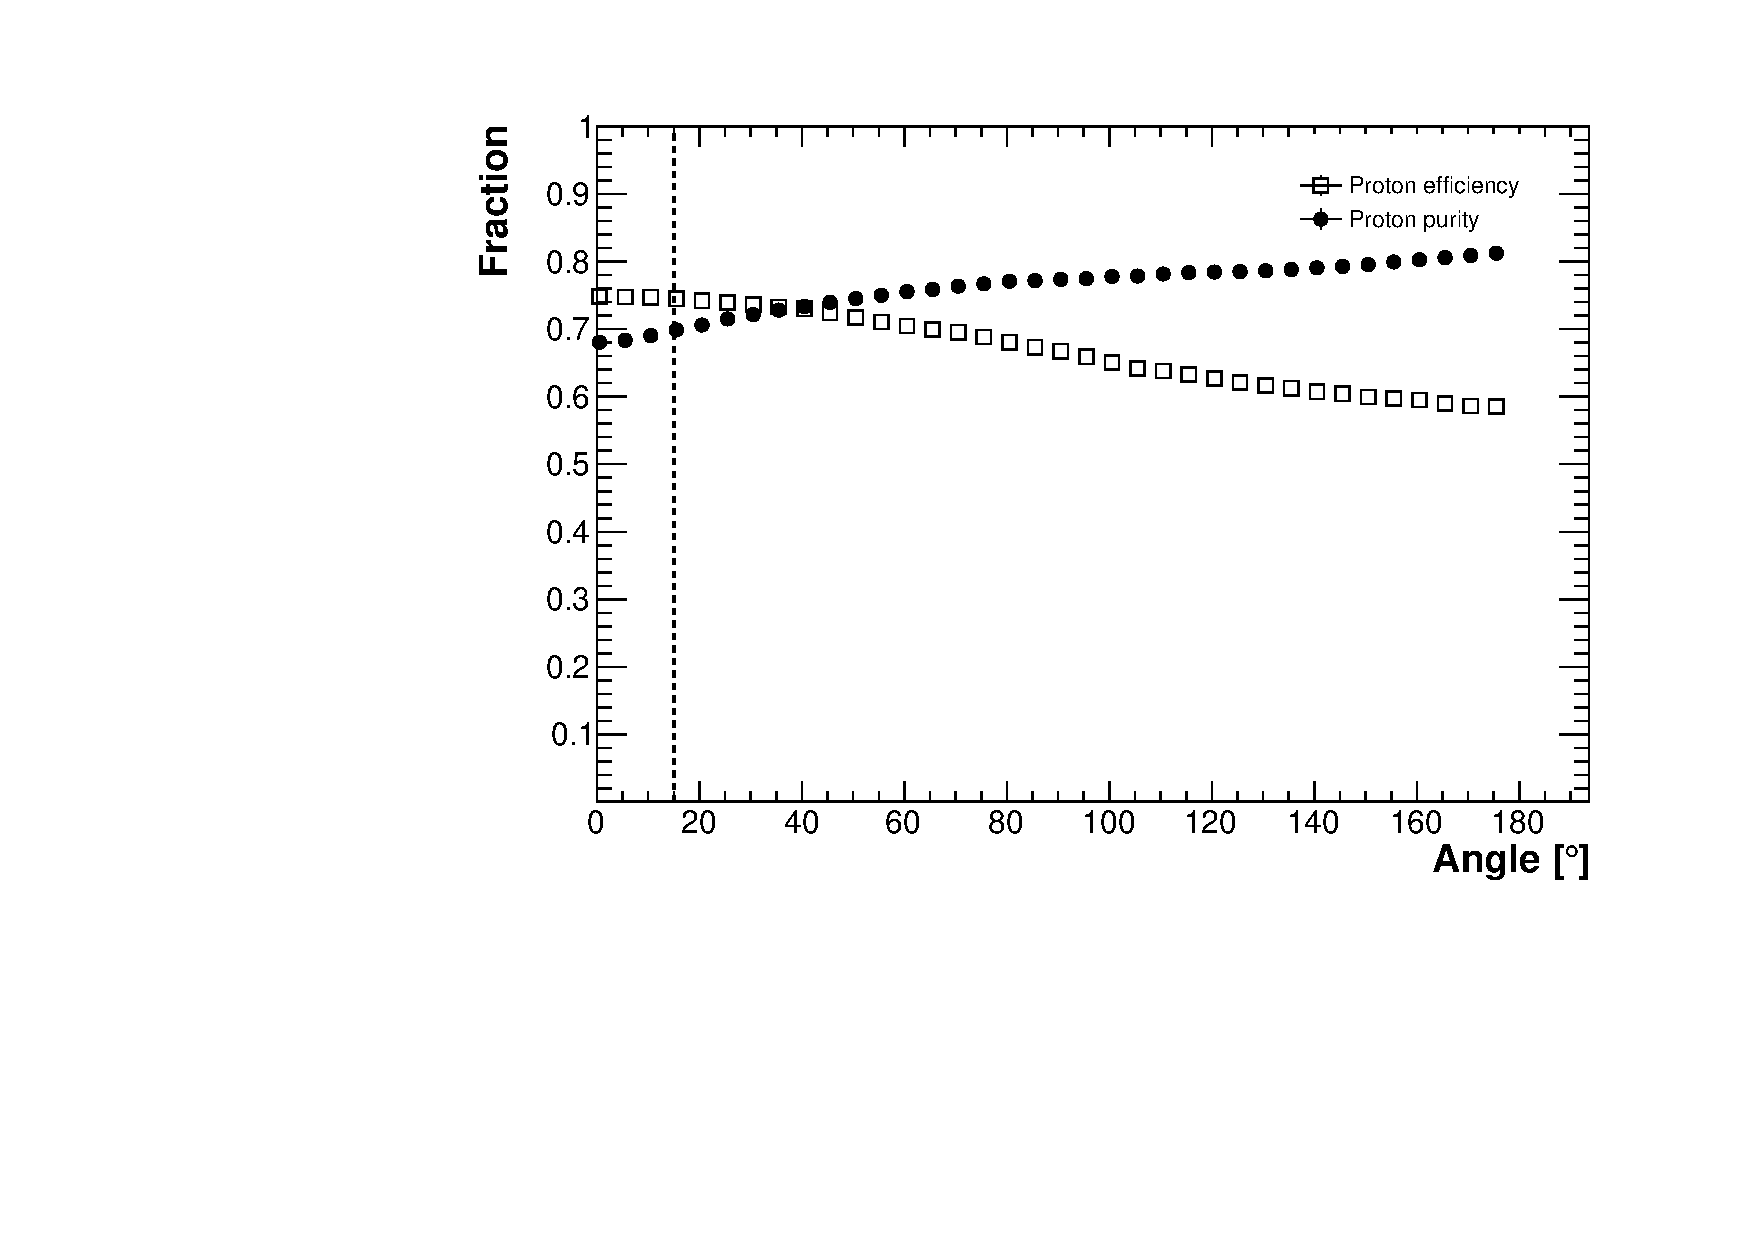
\includegraphics[width=0.65\linewidth]{figures/proton_angle.pdf}
  \caption{Proton reconstruction efficiency and purity as a function of the angular separation reclassification threshold.}
  \label{fig:showerangle}
\end{figure}

It is also possible for a small electron shower remnant to be reconstructed as a track-like object. Thus, we reclassify a track-like object as a shower if it is within the cone of the most energetic shower. This criterion correctly identifies a shower remnant in the 98.9\% of the cases.

\begin{figure}[htbp]
\centering
  \begin{subfigure}{0.45\textwidth}
    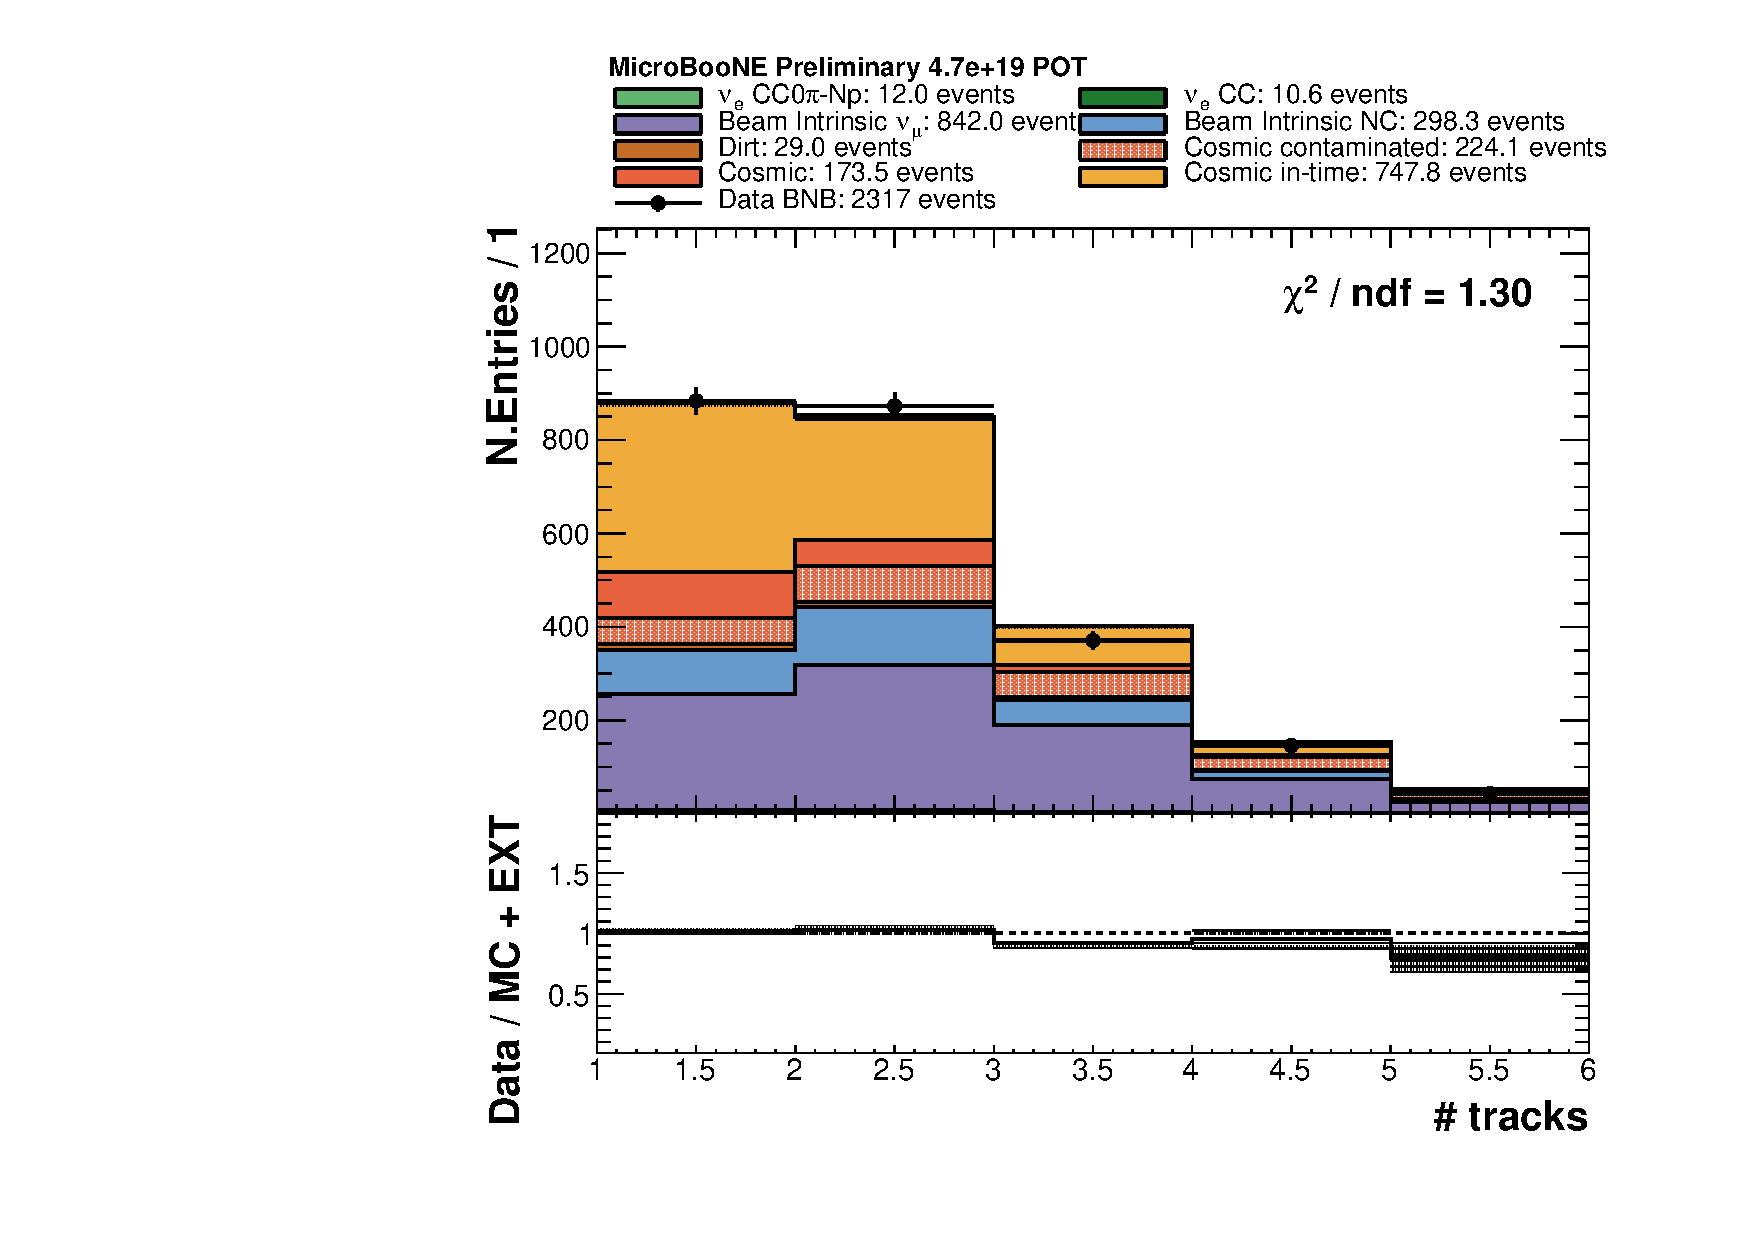
\includegraphics[width=\linewidth]{figures/h_n_tracks.pdf}
    \caption{Number of tracks.} 
  \end{subfigure}
    \begin{subfigure}{0.45\textwidth}
    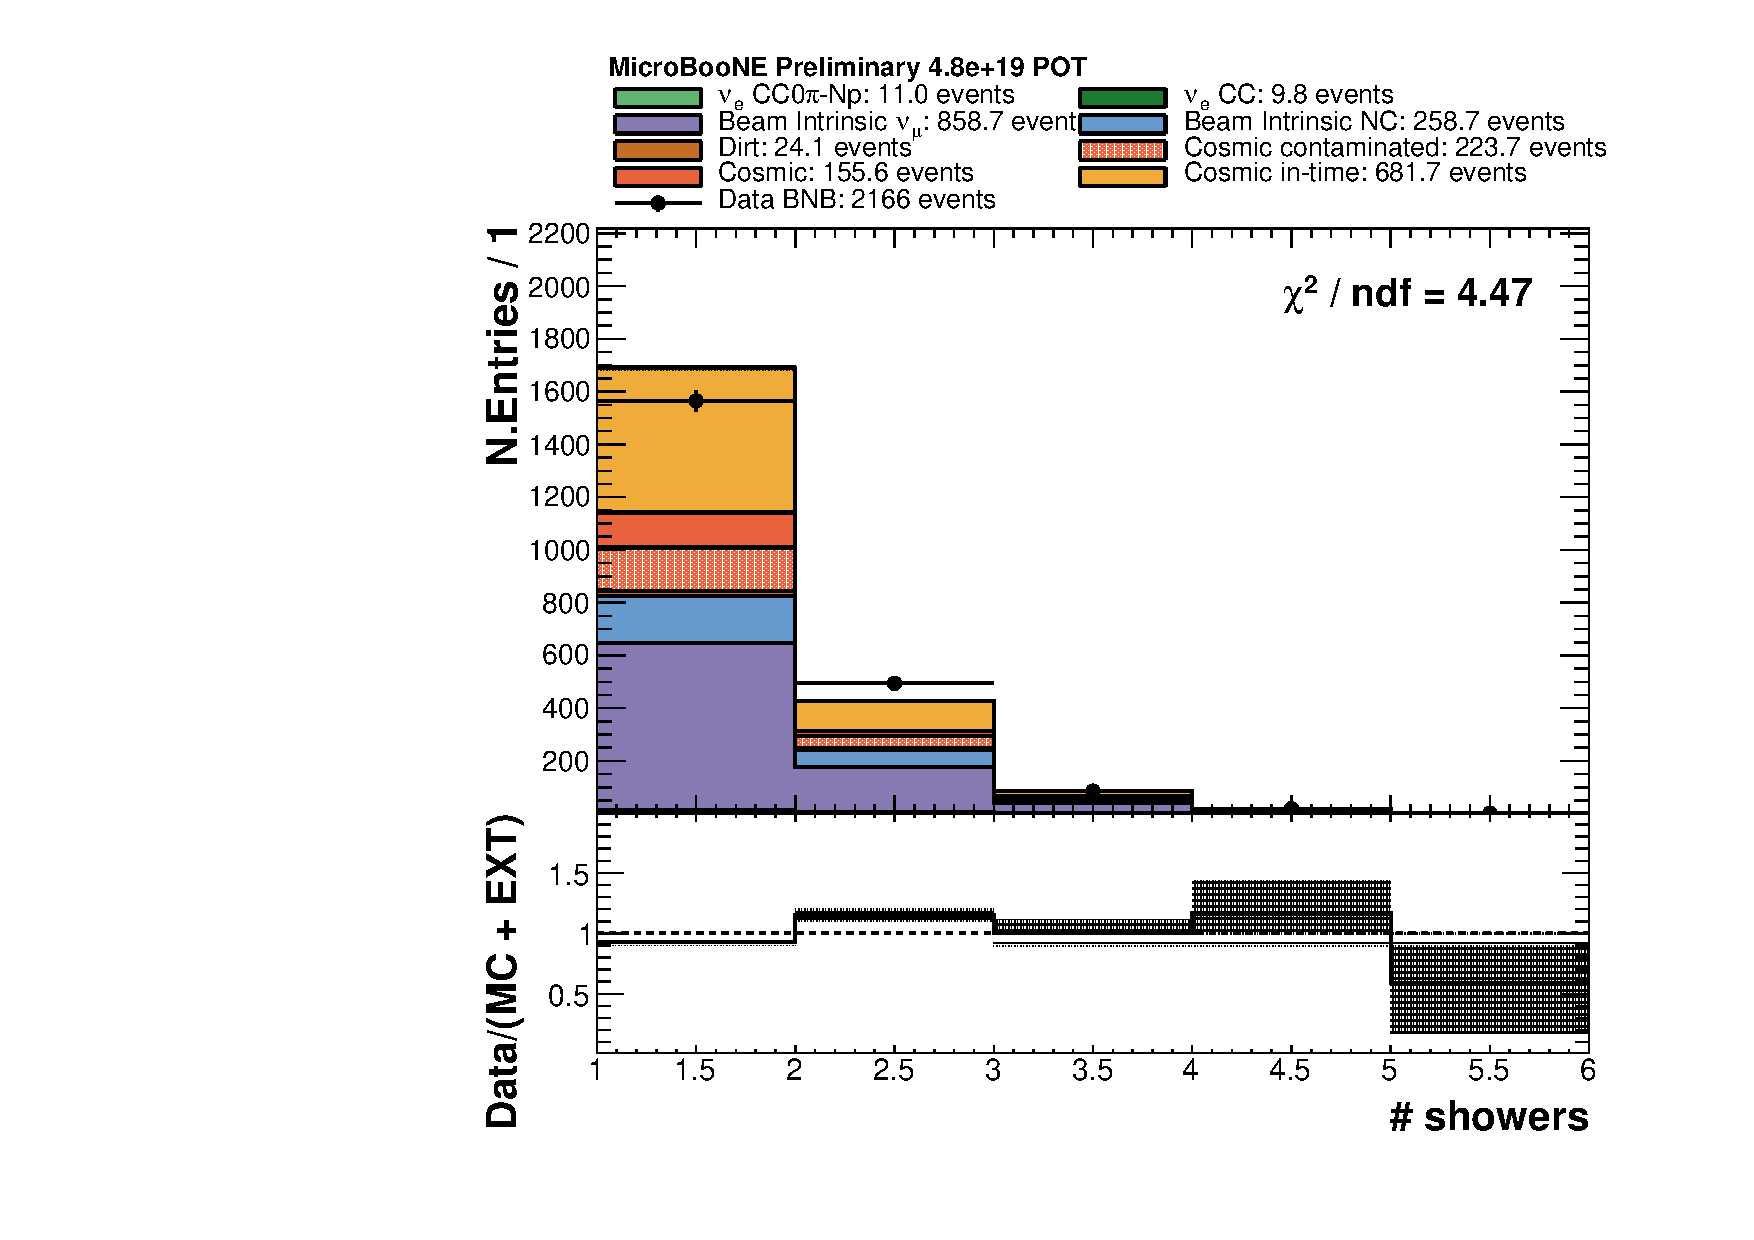
\includegraphics[width=\linewidth]{figures/h_n_showers.pdf}
    \caption{Number of showers.} 
  \end{subfigure}
  \caption{Number of tracks and number of showers per event after the reclassification procedure.}\label{fig:nshowers_after}
\end{figure}

Figure \ref{fig:nshowers_after} shows the number of shower-like objects and the number of track-like objects per event after these two reclassification procedures. The agreement improves and the bias in the ratio disappears. 

\subsection{Background Rejection}\label{sec:bkg}
\subsubsection{Introduction}
In this section we will describe the cuts applied to our selected sample, in order to isolate the $\nu_{e}$ CC$0\pi$-Np event candidates. The cuts have been chosen to (1) reduce the background, and (2) ensure that the selected events are well reconstructed. The values of each cut have been chosen manually. It would have been possible, in theory, to calculate an optimal set of cuts, maximized by the significance of the $\nu_{e}$ CC0$\pi$-Np events. However, this set of cuts would not have allowed a correct validation of the final selected sample, due to the limited size of the data unblinded sample. As such, the chosen cuts increase the purity of our sample, but also retain a significant amount ($\approx 20$) of selected data events.

\subsubsection{Shower \texorpdfstring{$dE/dx$}{dE/dx}}
The rate of energy loss per length ($dE/dx$) for electromagnetic showers is measured with a procedure analogous to the one described in \cite{argoneut}. All the hits of the collection plane within a rectangle of 4~cm along the direction of the shower and 1~cm perpendicular to the shower are collected. Figure \ref{fig:evddedx} shows a Monte Carlo event display with an electron shower and the rectangle used to measure the $dE/dx$.

\begin{figure}[htbp]
\centering
  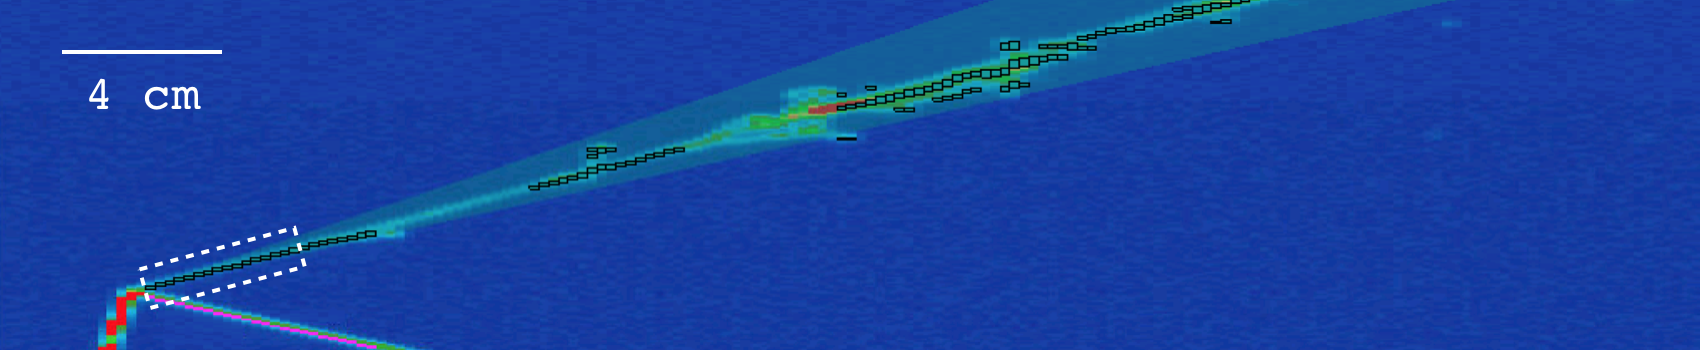
\includegraphics[width=0.9\linewidth]{figures/evddedx.png}
  \caption{Monte Carlo event display of an electron shower in the collection plane with the $1\times4$~cm rectangle used to measure the $dE/dx$. The black boxes correspond to the reconstructed hits.}
  \label{fig:evddedx}
\end{figure}

The $dQ/dx$ for each hit is measured dividing the collected charge ($dQ$) by the pitch ($dx$) between each hit and the next one along the shower direction. The pitch corresponds to the distance in the TPC that a particle travels between its two projections  on adjacent wires, which is \emph{at least} the wire spacing (3~mm for MicroBooNE \cite{detector}). 

The $dE/dx$ is calculated from the $dQ/dx$ by using the calibration factor measured in \eqref{eq:calib}.
Since the distribution of the $dE/dx$ hit values has an asymmetric tail due to the Landau nature of the process, we assign to the shower the median (and not the mean) of the $dE/dx$ hit distribution.

Figure \ref{fig:dedx} shows the $dE/dx$ hit distribution and the $dE/dx$ median distribution for electron and photon showers obtained with a Monte Carlo simulation. In this plot, each shower is required to have at least 10 reconstructed hits. As expected, the electron distribution is peaked around 2~MeV/cm. The photon distribution has two peaks, one around 2~MeV/cm and one around 4~MeV/cm. 


\begin{figure}[htbp]
\centering
  \begin{subfigure}{0.45\textwidth}
    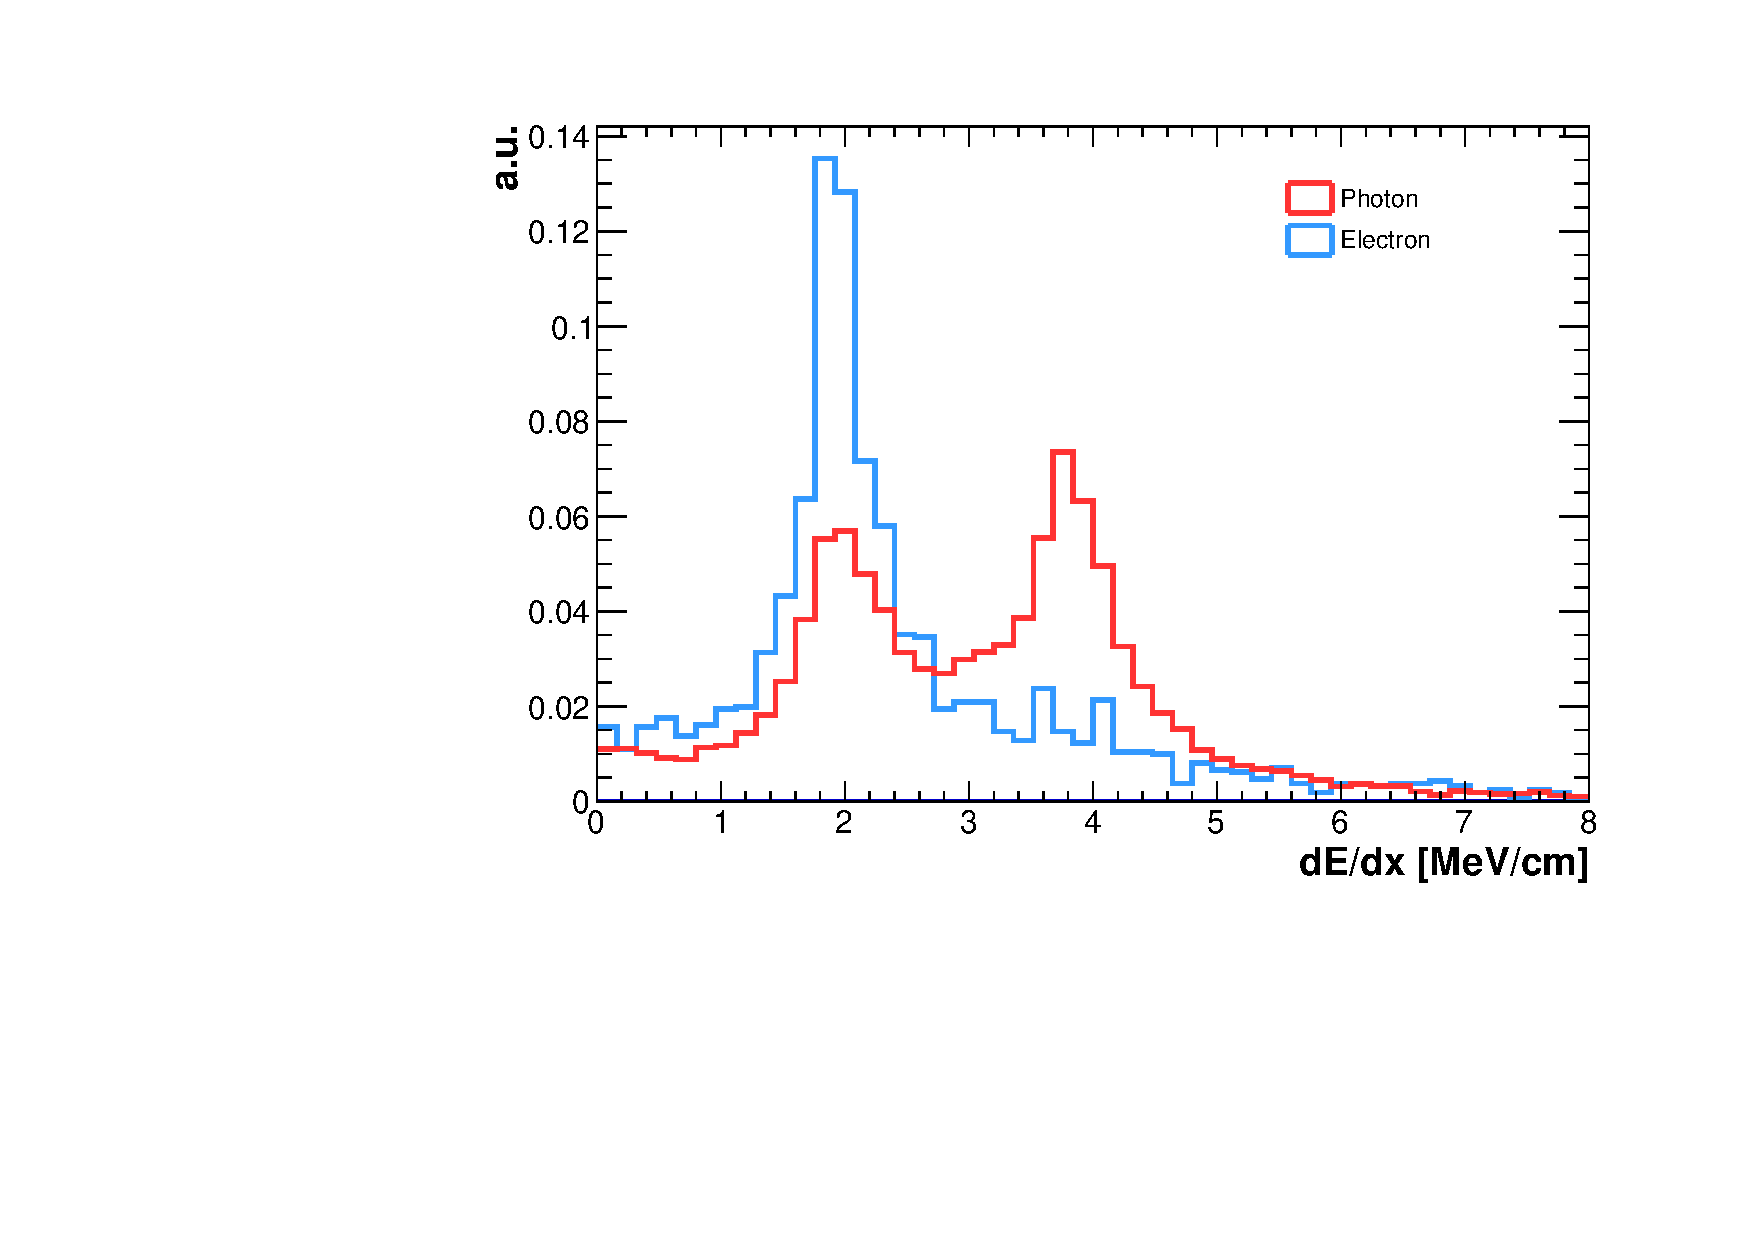
\includegraphics[width=\linewidth]{figures/dedx.pdf}
    \caption{$dE/dx$ median distribution} 
  \end{subfigure}
    \begin{subfigure}{0.45\textwidth}
    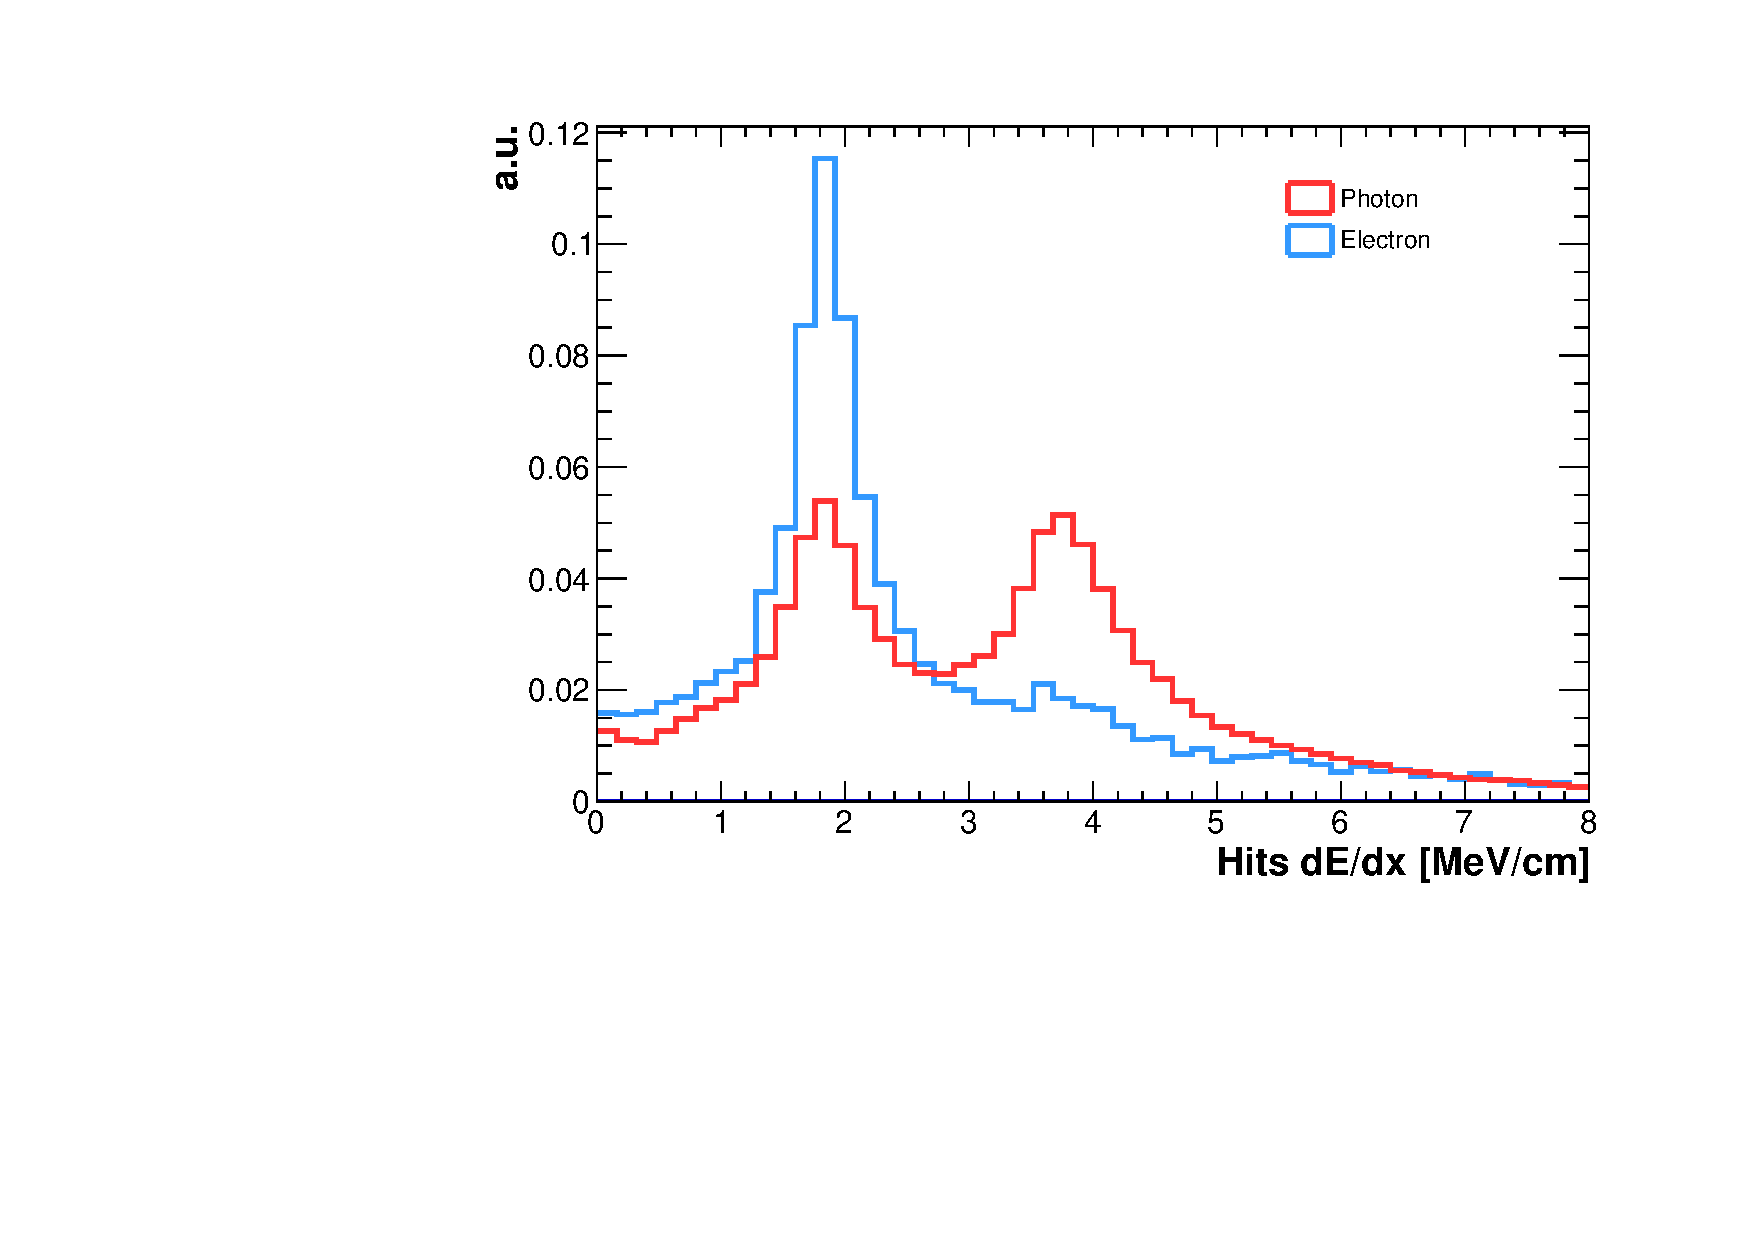
\includegraphics[width=\linewidth]{figures/hits_dedx.pdf}
    \caption{$dE/dx$ hit distribution} 
  \end{subfigure}
  \caption{$dE/dx$ median distribution (left) and the $dE/dx$ hit distribution (right) for electron and photon showers with at least 10 reconstructed hits.}\label{fig:dedx}
\end{figure}


The first peak is caused by low-energy photons and, to a lesser extent, Compton scattering. When a low energetic photon converts into a $e^+e^-$ pair, in the case of a very asymmetric decay, the electron (or the positron) can have a very low deposited energy. In this case, one of the two particle will travel for a much shorter distance than the 4~cm rectangle length, causing the median of the distribution to be 2~MeV/cm and not 4~MeV/cm \cite{caratelli}. Figure \ref{fig:dedx_energy} shows a bi-dimensional histogram of the $dE/dx$ vs. the reconstructed energy for simulated photon showers: as expected, the first peak is mainly caused by low-energy showers. In our sample, the cut applied on the most energetic shower is $1~\mathrm{MeV/cm} < dE/dx < 3.2~\mathrm{MeV/cm}$.


\begin{figure}[htbp]
\centering
  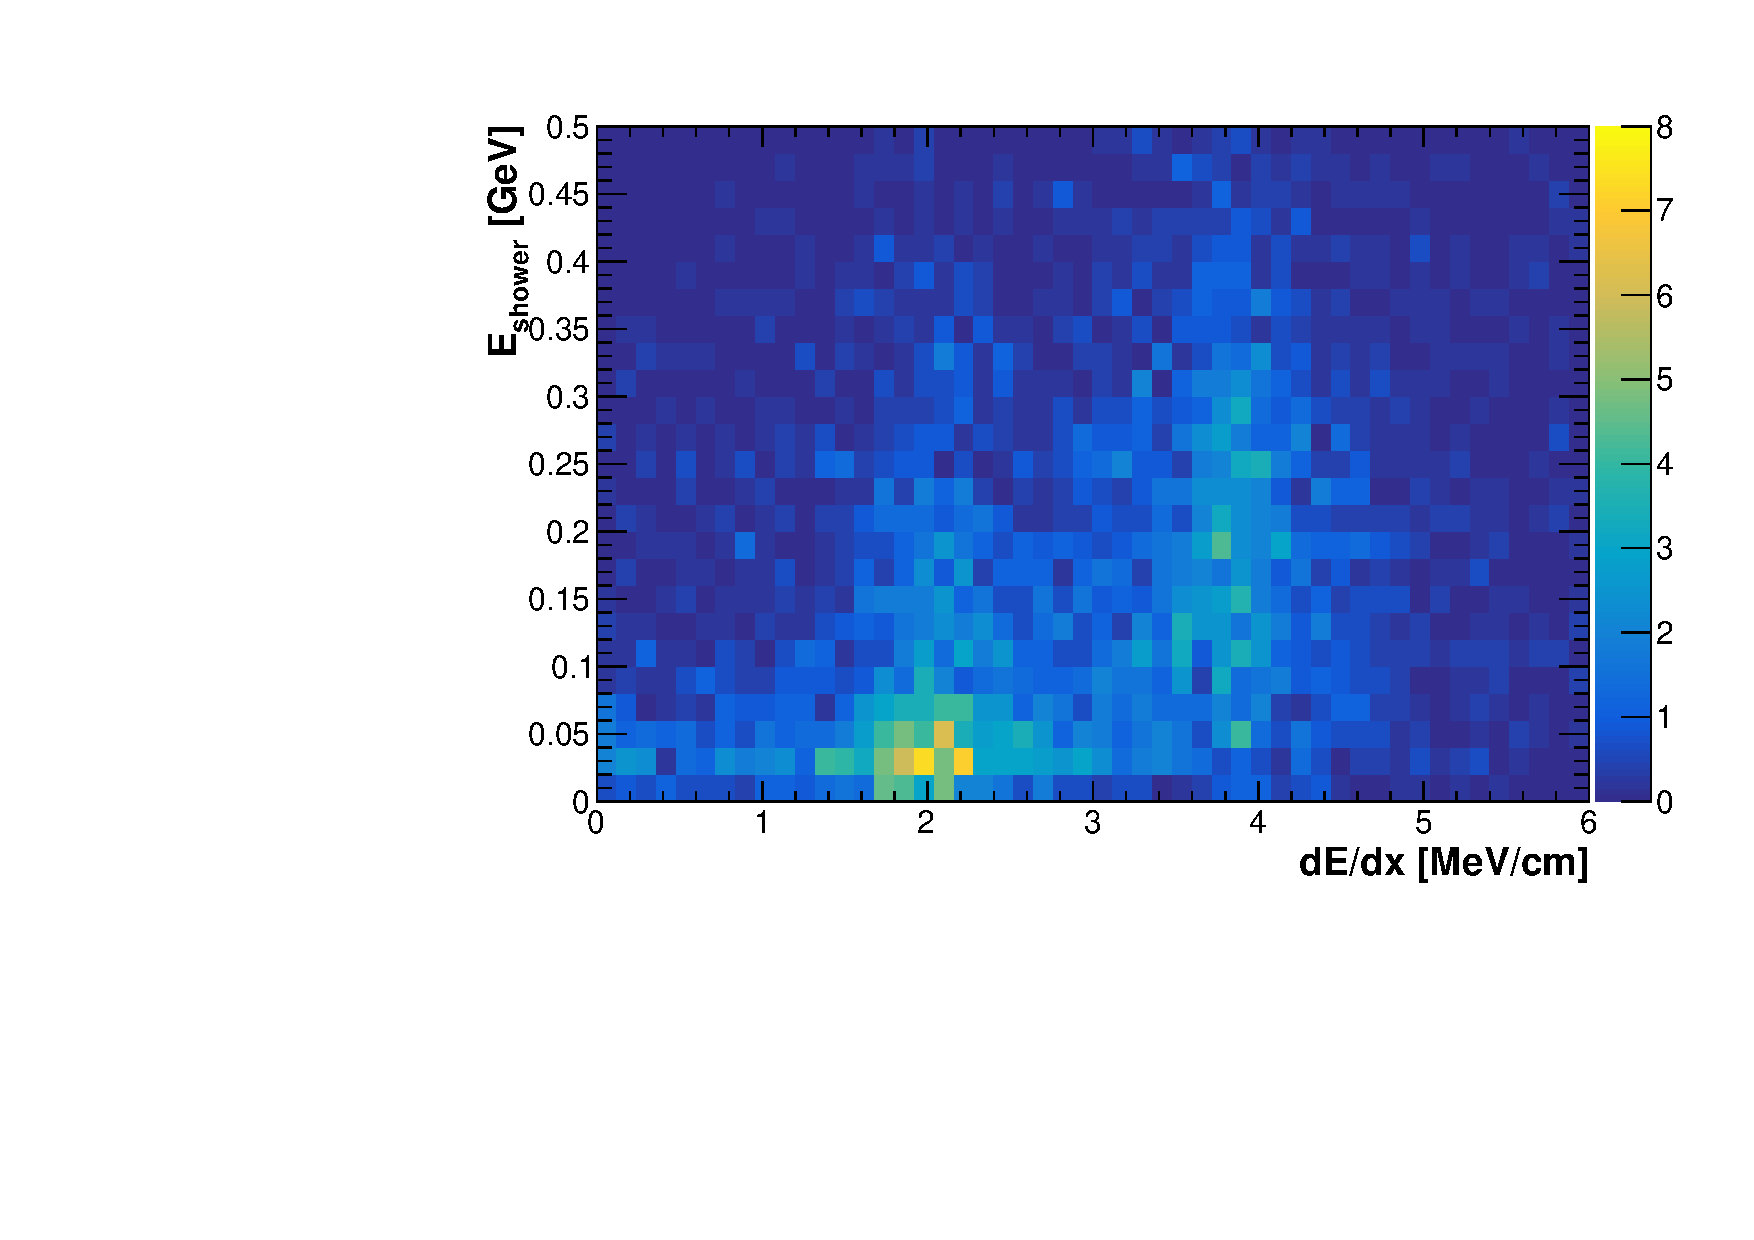
\includegraphics[width=0.7\linewidth]{figures/dedx_energy.pdf}
  \caption{$dE/dx$ vs. reconstructed shower energy $E_{\mathrm{shower}}$ for photon showers. The peak around 2 MeV/cm corresponds mainly to low-energy showers.}\label{fig:dedx_energy}
\end{figure}


\subsubsection{Shower energy}
The energy of each electromagnetic shower is measured with the procedure described in Section \ref{sec:showerenergy}. A large number of cosmic in-time events will have a low shower energy, mainly caused by Michel electrons. A significant portion of charged-current $\nu_{\mu}$ events will also have low-energy showers caused by stopping muons and spurious hits. A cut of 50 MeV on the reconstructed energy of the most energetic shower removes a large fraction of the cosmic in-time and CC $\nu_{\mu}$ backgrounds, without significantly reducing the $\nu_{e}$ CC0$\pi$-Np efficiency. 
% Figure \ref{fig:showerenergy} shows the reconstructed energy distribution of the most energetic shower in the low-energy region and the reconstructed energy spectrum after the shower energy cut.

\subsubsection{Track distance}
A well reconstructed event with a proton in the final state will have a reconstructed track close to the reconstructed neutrino vertex. However, the requirement on the distance between the reconstructed track and the reconstructed neutrino vertex can not be too strict, due to the limited neutrino vertex spatial resolution. Figure \ref{fig:dist} shows the histogram of the distance between the true neutrino vertex (corrected by the space-charge effect \cite{sce}) and the reconstructed neutrino vertex for simulated $\nu_{e}$ CC0$\pi$-Np events. Each reconstructed track is required to be within 3~cm the reconstructed neutrino vertex.

\begin{figure}[htbp]
\centering
  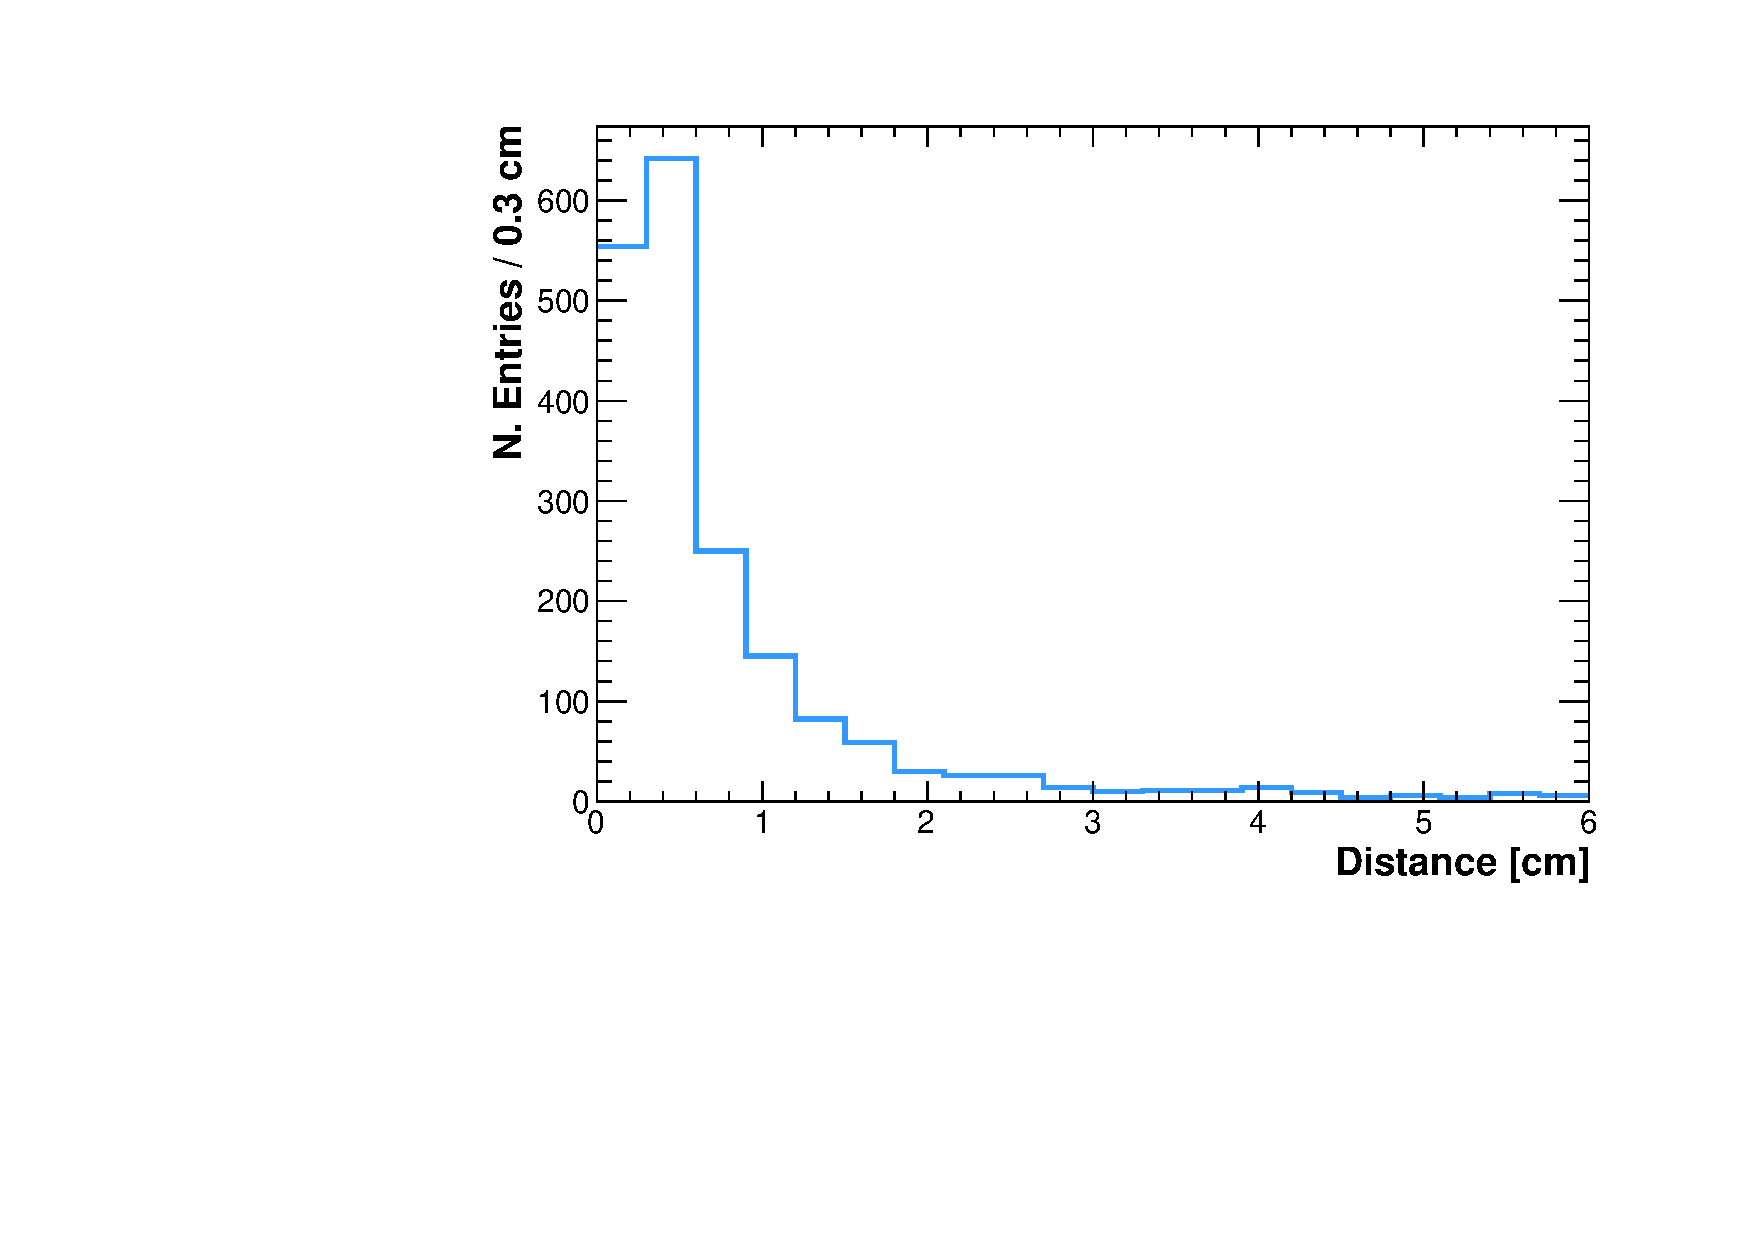
\includegraphics[width=0.7\linewidth]{figures/dist.pdf}
  \caption{Distance between the reconstructed neutrino vertex and the true neutrino vertex, corrected by the space-charge effect, for $\nu_{e}$ CC0$\pi$-Np simulated events.}\label{fig:dist}
\end{figure}

\subsubsection{Proton track BDT}\label{sec:protbdt}
The aim of the analysis is to find $\nu_{e}$ CC$0\pi$-Np events. As such, it is necessary to identify events with non-proton tracks in the final state (e.g. pions and muons). A boosted decision tree (BDT) has been trained using the length of the track and its $dQ/dx$. In the training sample, the signal corresponds to reconstructed tracks matched to protons and the background to reconstructed tracks matched to muons. Figure \ref{fig:bdt} shows the $dQ/dx$ as a function of the track length and the BDT score for proton tracks and muon tracks. Each track in the event candidate must have a BDT score of at least -0.12, which corresponds to a signal efficiency of 98\% and a background rejection of 55\%. 

\begin{figure}[htbp]
\centering
  \begin{subfigure}{0.45\textwidth}
    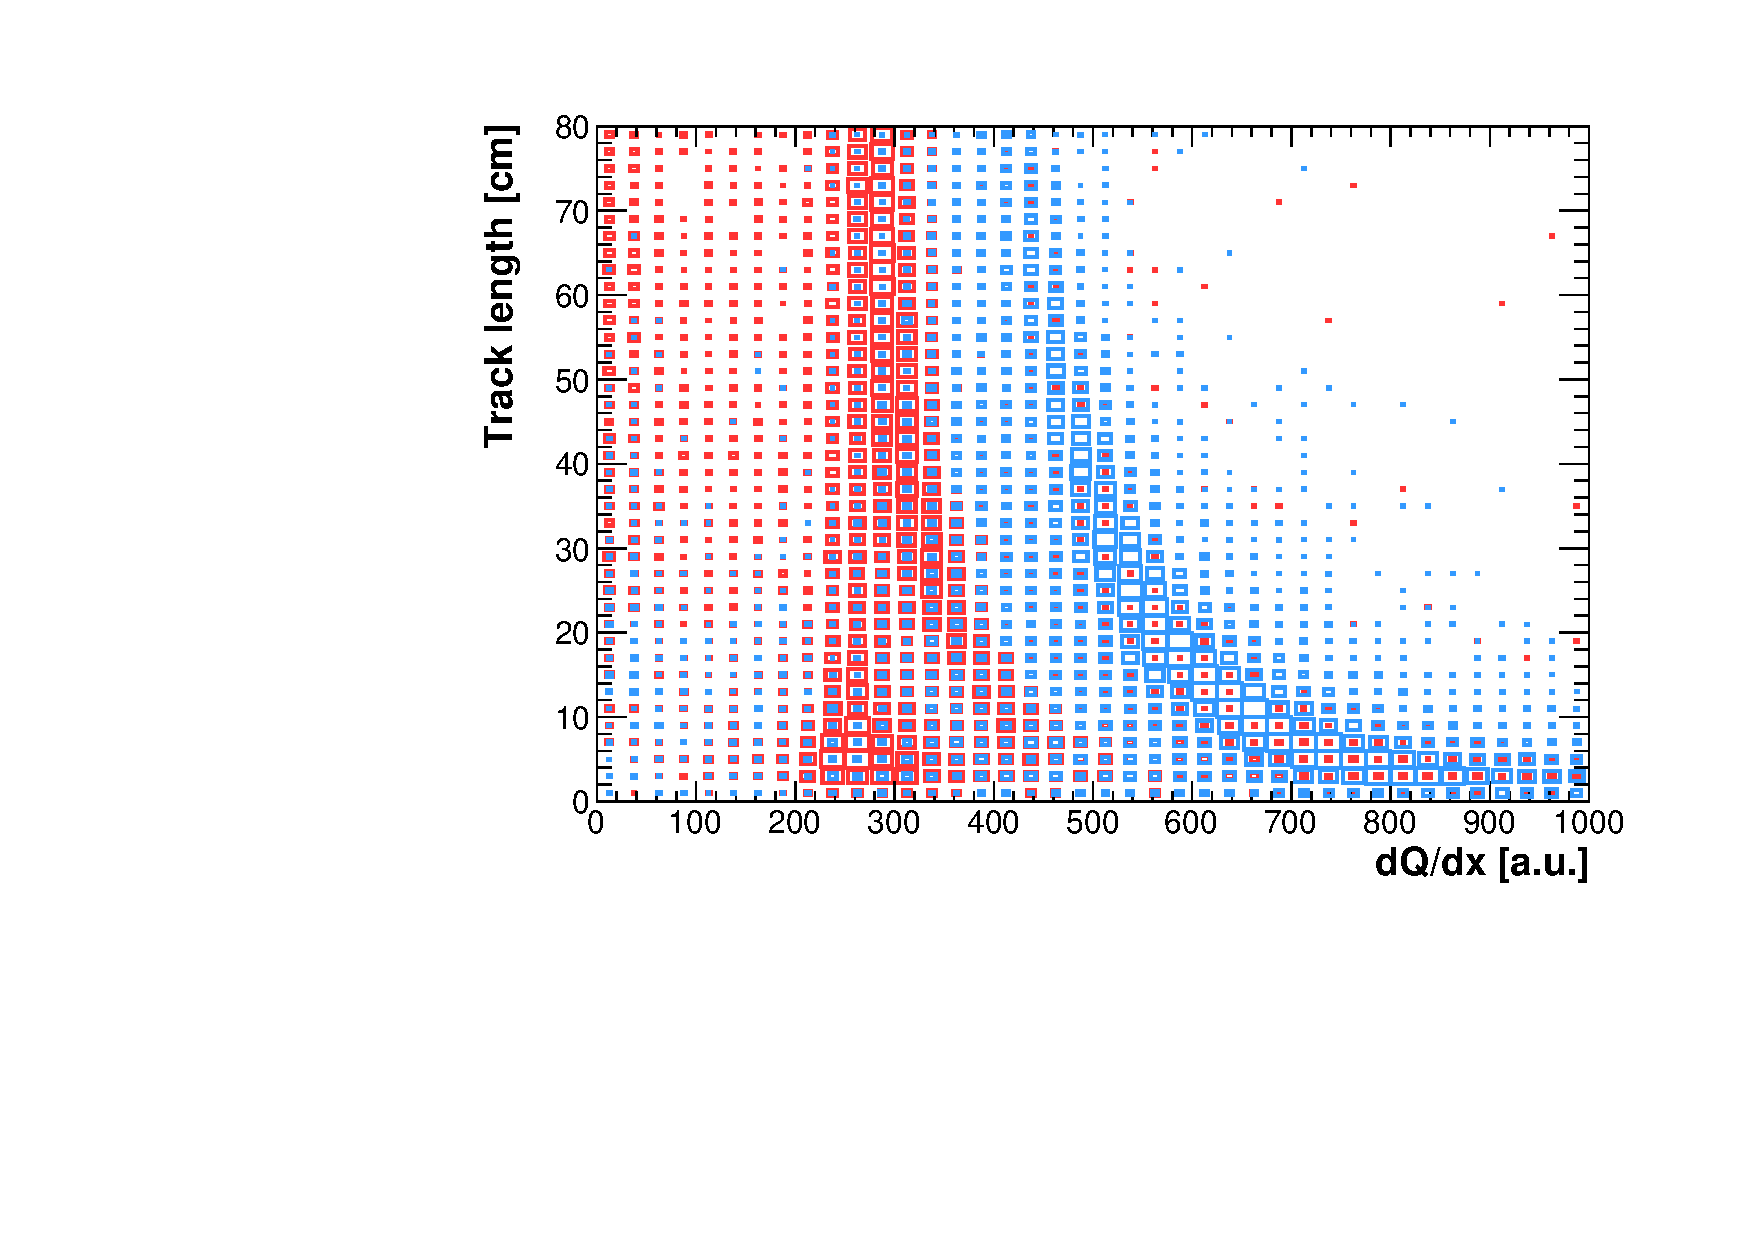
\includegraphics[width=\linewidth]{figures/dqdx.pdf}
    \caption{$dQ/dx$ as a function of track length.} 
  \end{subfigure}
    \begin{subfigure}{0.45\textwidth}
    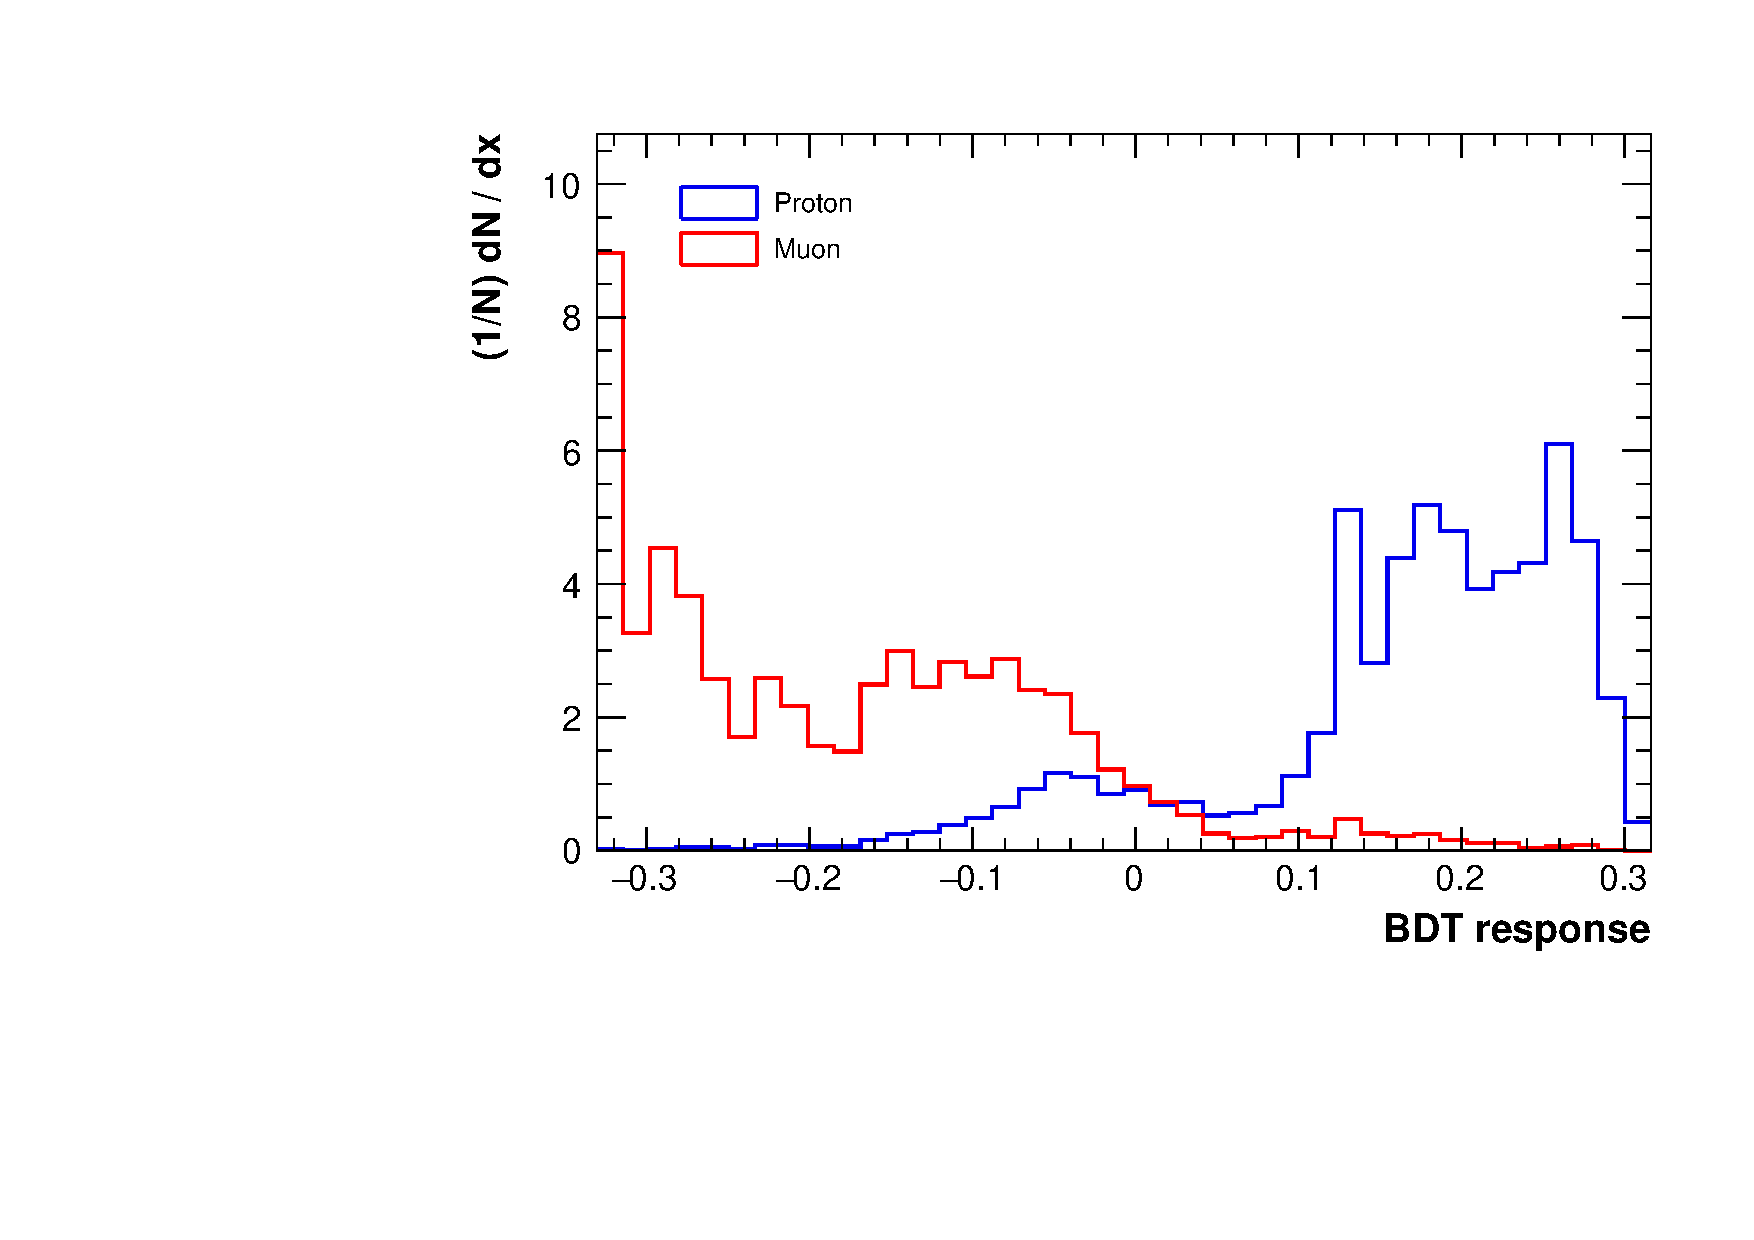
\includegraphics[width=\linewidth]{figures/bdt.pdf}
    \caption{BDT score.} 
  \end{subfigure}
  \caption{Proton-like tracks are chosen from the score of a boosted decision tree, trained using the track length and the $dQ/dx$ for reconstructed protons (blue) and muons (red).}\label{fig:bdt}
\end{figure}

\subsubsection{Track-shower angle}
Low-energy electrons often start producing an appreciable shower in the detector after several centimeters. As such, the reconstruction framework identifies the first part of the shower as a track-like object and the last part of the shower as a shower-like object. 
Furthermore, high-energy cosmic rays can produce a shower in the detector, which will be mostly aligned to the track. In order to remove these mis-reconstructed events and reduce this kind of cosmogenic background we require $\mathrm{cos}\theta > -0.9$, where $\theta$ is the angle between the most energetic shower and the most proton-like track, as identified by the procedure described in Section \ref{sec:protbdt}.
Figure \ref{fig:angle} shows the event displays of a cosmic ray showering in the last part and of an electron shower being reconstructed as a track-like object plus a shower-like object.

\begin{figure}[htbp]
\centering
  \begin{subfigure}{0.45\textwidth}
    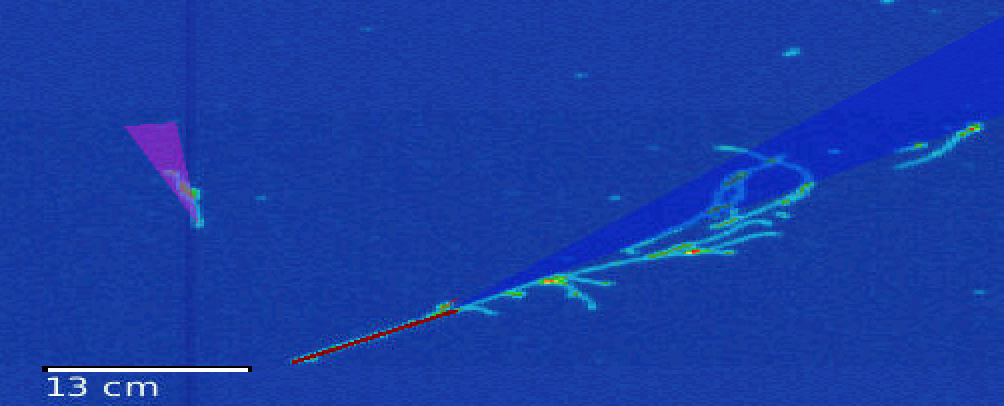
\includegraphics[width=\linewidth]{figures/angle1.png}
    \caption{Cosmic-ray shower} 
  \end{subfigure}
    \begin{subfigure}{0.45\textwidth}
    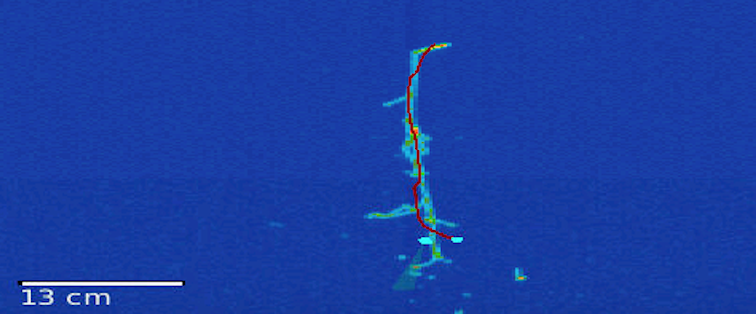
\includegraphics[width=\linewidth]{figures/angle2.png}
    \caption{Electron shower} 
  \end{subfigure}
  \caption{Monte Carlo event displays of a cosmic ray showering in the detector (left) and of an electron shower (right). Both objects were reconstructed in the first part as a track-like object and in the last part as a shower-like object}\label{fig:angle}
\end{figure}


\subsubsection{Shower opening angle}
Reconstructed showers corresponding to low-energy electrons will have in general a small opening angle $\theta$. Requiring the most energetic shower to be smaller than $20^{\circ}$ and larger than $1^{\circ}$ allows to reduce the background component without significantly impacting the signal efficiency. In this way we are able to reject $\nu_{\mu}$ CCDIS events and high-energetic cosmic-ray events, which will have larger opening angles. The requirement on the minimum value of the opening angle allows also to reject events with tracks mis-reconstructed as shower-like objects.

\subsubsection{Track length}
Our signal sample will contain only protons in the final state. Protons in liquid argon have a higher stopping power than muons, which will correspond on average to shorter tracks. Each reconstructed track in the selected sample is required to be shorter than 80 cm. This cut helps rejecting mainly CC $\nu_{\mu}$ events with high-energy muons in the final state.
Thus, an increased size of the unblinded data sample could allow us to apply more efficient cuts.

% \subsection{Optical selection}


% \subsection{Topology requirement}
